%%%%%%%%%%%%%%%%%%%%%%%%%%%%%%%%%%%%%%%%%%%%%%%%%%%%%%%%%%%%%%%%%%%%%%%%
%% Customizações do abnTeX2 (http://abnTeX2.googlecode.com)           %%
%% para a Universidade Estadual do Ceara - UECE                       %%
%%                                                                    %%
%% This work may be distributed and/or modified under the             %% 
%% conditions of the LaTeX Project Public License, either version 1.3 %%
%% of this license or (at your option) any later version.             %%
%% The latest version of this license is in                           %%
%%   http://www.latex-project.org/lppl.txt                            %%
%% and version 1.3 or later is part of all distributions of LaTeX     %%
%% version 2005/12/01 or later.                                       %%
%%                                                                    %%
%% This work has the LPPL maintenance status `maintained'.            %%
%%                                                                    %%
%% The Current Maintainer of this work is Thiago Nascimento           %%
%%                                                                    %%
%% Project available on: https://github.com/thiagodnf/uecetex2        %%
%%                                                                    %%
%% Further information about abnTeX2                                  %%
%% are available on http://abntex2.googlecode.com/                    %%
%%                                                                    %%
%%%%%%%%%%%%%%%%%%%%%%%%%%%%%%%%%%%%%%%%%%%%%%%%%%%%%%%%%%%%%%%%%%%%%%%%

\input{lib/preambulo}
\tikzset{
  vec/box/.style={draw, rounded corners=2pt, thick, align=center, inner sep=4pt},
  vec/small/.style={draw, rounded corners=2pt, thick, align=center, inner sep=2pt, font=\small},
  vec/arrow/.style={-Latex, thick},
  vec/darrow/.style={<->, Latex-Latex, thick},
  vec/dot/.style={circle, fill, inner sep=1.3pt},
  vec/title/.style={font=\small\bfseries, align=center},
  vec/note/.style={font=\footnotesize, align=left},
  vec/cloud/.style={draw, thick, cloud, cloud puffs=12, cloud puff arc=110, aspect=2, align=center, inner sep=4pt},
  vec/tower/.style={draw, thick, isosceles triangle, isosceles triangle apex angle=25, shape border rotate=90, minimum height=10mm, minimum width=10mm, align=center},
  vec/server/.style={draw, thick, rounded corners=2pt, minimum width=18mm, minimum height=10mm, align=center},
}



%%%%%%%%%%%%%%%%%%%%%%%%%%%%%%%%%%%%%%%%%%%%%%%%%%%%%
%%          Configuracoes do ueceTeX2              %%
%%%%%%%%%%%%%%%%%%%%%%%%%%%%%%%%%%%%%%%%%%%%%%%%%%%%%

% Opcoes disponiveis

%\trabalhoacademico{tccgraduacao}
%\trabalhoacademico{tccespecializacao}
% \trabalhoacademico{dissertacao}
\trabalhoacademico{tese}

% Define se o trabalho eh uma qualificacao
% Coloque 'nao' para versao final do trabalho

\ehqualificacao{sim}

% Remove as bordas vermelhas e verdes do PDF gerado
% Coloque 'sim' pare remover

\removerbordasdohyperlink{sim} 

% Adiciona a cor Azul a todos os hyperlinks

\cordohyperlink{nao}

%%%%%%%%%%%%%%%%%%%%%%%%%%%%%%%%%%%%%%%%%%%%%%%%%%%%%
%%          Informação sobre a IES                 %%
%%%%%%%%%%%%%%%%%%%%%%%%%%%%%%%%%%%%%%%%%%%%%%%%%%%%%

\ies{Universidade Estadual do Ceará}
\iessigla{UECE}
\centro{Centro de Ciências e Tecnologia}

%%%%%%%%%%%%%%%%%%%%%%%%%%%%%%%%%%%%%%%%%%%%%%%%%%%%%
%%        Informação para TCC de Graduacao         %%
%%%%%%%%%%%%%%%%%%%%%%%%%%%%%%%%%%%%%%%%%%%%%%%%%%%%%

\graduacaoem{Ciência da Computação}
\habilitacao{bacharel} % Pode colocar tambem 'licenciada'

%%%%%%%%%%%%%%%%%%%%%%%%%%%%%%%%%%%%%%%%%%%%%%%%%%%%%
%%     Informação para TCC de Especializacao       %%
%%%%%%%%%%%%%%%%%%%%%%%%%%%%%%%%%%%%%%%%%%%%%%%%%%%%%

\especializacaoem{Alfabetização de Crianças}

%%%%%%%%%%%%%%%%%%%%%%%%%%%%%%%%%%%%%%%%%%%%%%%%%%%%%
%%         Informação para Dissertacao             %%
%%%%%%%%%%%%%%%%%%%%%%%%%%%%%%%%%%%%%%%%%%%%%%%%%%%%%

\programamestrado{Programa de Pós-Graduação em Ciência da Computação}
\nomedomestrado{Mestrado Acadêmico em Ciência da Computação}
\mestreem{Ciência da Computação}
\areadeconcentracaomestrado{Ciência da Computação}

%%%%%%%%%%%%%%%%%%%%%%%%%%%%%%%%%%%%%%%%%%%%%%%%%%%%%
%%               Informação para Tese              %%
%%%%%%%%%%%%%%%%%%%%%%%%%%%%%%%%%%%%%%%%%%%%%%%%%%%%%

\programadoutorado{Programa de Pós-Graduação em Ciência da Computação}
\nomedodoutorado{Doutorado em Ciência da Computação}
\doutorem{Ciência da Computação}
\areadeconcentracaodoutorado{Redes de Computadores}

%%%%%%%%%%%%%%%%%%%%%%%%%%%%%%%%%%%%%%%%%%%%%%
%%  Informação relacionadas ao trabalho     %%
%%%%%%%%%%%%%%%%%%%%%%%%%%%%%%%%%%%%%%%%%%%%%%

\autor{Antônio Sérgio de Sousa Vieira}
\titulo{SAC-FTOPSIS: Um Modelo de Decisão para o Descarregamento de Tarefas em Redes Veiculares}
\data{2026}
\local{Fortaleza -- Ceará}

% Exemplo: \dataaprovacao{01 de Janeiro de 2012}
\dataaprovacao{}

%%%%%%%%%%%%%%%%%%%%%%%%%%%%%%%%%%%%%%%%%%%%%
%%     Informação sobre o Orientador       %%
%%%%%%%%%%%%%%%%%%%%%%%%%%%%%%%%%%%%%%%%%%%%%

\orientador{Dr. Joaquim Celestino Júnior}
\orientadories{Universidade Estadual do Ceará – UECE}
\orientadorcentro{Centro de Ciências e Tecnologia - CCT}
\orientadorfeminino{nao} % Coloque 'sim' se for do sexo feminino

%%%%%%%%%%%%%%%%%%%%%%%%%%%%%%%%%%%%%%%%%%%%%
%%      Informação sobre o Co-orientador   %%
%%%%%%%%%%%%%%%%%%%%%%%%%%%%%%%%%%%%%%%%%%%%%

% Deixe o nome do coorientador em branco para remover do documento

\coorientador{Prof. Dr. Alisson Barbosa de Souza}
\coorientadories{Universidade Federal do Ceará – UFC}
\coorientadorcentro{Centro de Ciências e Tecnologia - CCT}
\coorientadorfeminino{nao} % Coloque 'sim' se for do sexo feminino

%%%%%%%%%%%%%%%%%%%%%%%%%%%%%%%%%%%%%%%%%%%%%
%%      Informação sobre a banca           %%
%%%%%%%%%%%%%%%%%%%%%%%%%%%%%%%%%%%%%%%%%%%%%

% Atenção! Deixe o nome do membro da banca para remover da folha de aprovacao

% Exemplo de uso:
% \membrodabancadois{Prof. Dr. Fulano de Tal}
% \membrodabancadoisies{Universidade Estadual do Ceará - UECE}

\membrodabancadois{Prof. Dr. Luís Manuel De Jesus Sousa Correia}
\membrodabancadoiscentro{Centro de Ciências e Tecnologia - CCT}
\membrodabancadoisies{Universidade de Lisboa - ULisboa}
\membrodabancatres{Prof. Dr. Gustavo Augusto Lima de Campos}
\membrodabancatrescentro{Centro de Ciências e Tecnologia - CCT}
\membrodabancatresies{Universidade Estadual do Ceará – UECE}
\membrodabancaquatro{Prof. Dr. Eduardo de Olivindo Cavalcante}
\membrodabancaquatrocentro{Centro de Ciências e Tecnologia - CCT}
\membrodabancaquatroies{Instituto Federal de Educação, Ciência e Tecnologia do Ceará – IFCE}
\membrodabancacinco{}
\membrodabancacincocentro{}
\membrodabancacincoies{}
\membrodabancaseis{}
\membrodabancaseiscentro{}
\membrodabancaseisies{}

\begin{document}	

	% Se o seu trabalho é em ingles, descomente a linha a seguir
	%\selectlanguage{english}

	% Elementos pré-textuais
	\imprimircapa
	\imprimirfolhaderosto{}
	% \imprimirfichacatalografica{elementos-pre-textuais/ficha-catalografica}
	% \imprimirerrata{elementos-pre-textuais/errata}
	\imprimirfolhadeaprovacao
	% \imprimirdedicatoria{elementos-pre-textuais/dedicatoria}
	% \imprimiragradecimentos{elementos-pre-textuais/agradecimentos}
	% \imprimirepigrafe{elementos-pre-textuais/epigrafe}
	\imprimirresumo{elementos-pre-textuais/resumo}
	\imprimirabstract{elementos-pre-textuais/abstract}
	\imprimirlistadeilustracoes
	\imprimirlistadetabelas
	% \imprimirlistadequadros
	% \imprimirlistadealgoritmos
	% \imprimirlistadecodigosfonte
	\imprimirlistadeabreviaturasesiglas	
	% \imprimirlistadesimbolos{elementos-pre-textuais/lista-de-simbolos}   
	\imprimirsumario
	
	% Reseta o primeiro uso das siglas para que sejam expandidas no texto principal
	\glsresetall
	
	%Elementos textuais
	\textual
	% !TeX root = ../documento.tex
\chapter{Introdução}
\label{cap:introducao}

Este capítulo apresenta uma visão geral do trabalho, descrevendo o contexto e os desafios que o motivaram (Seção~\ref{sec:contextualizacao} e Seção~\ref{sec:motivacao}). A partir disso, formaliza-se o problema de pesquisa (Seção~\ref{sec:definicao-do-problema}), as questões norteadoras (Seção~\ref{sec:questoes-de-pesquisa}) e as hipóteses elencadas (Seção~\ref{sec:hipoteses}). Por fim, são traçados os objetivos (Seção~\ref{sec:objetivos}), as contribuições esperadas (Seção~\ref{sec:contribuicoes}), as publicações decorrentes da pesquisa (Seção~\ref{sec:publicacao}) e a forma como o documento está estruturado (Seção~\ref{sec:organizacao}).

\section{Contextualização}
\label{sec:contextualizacao}

A convergência entre tecnologias de comunicação, eletrificação veicular e condução autônoma tem moldado um novo paradigma para o setor de transportes. O conceito de \gls{IoV} transforma veículos em sistemas computacionais sofisticados, capazes de viabilizar diversas aplicações de \gls{ITS}~\cite{RANI2023108543}. 

Veículos modernos são equipados com múltiplos sensores, unidades de processamento e interfaces de comunicação, permitindo a coleta e o processamento de grandes volumes de dados. Contudo, a complexidade das aplicações e a quantidade crescente de dados a serem processados podem exceder a capacidade computacional das \gls{OBU} instaladas.

Uma solução imediata seria aumentar a capacidade computacional dessas \glspl{OBU}, possibilitando maior processamento local. No entanto, o atual período de transição tecnológica resulta em cenários heterogêneos, no qual coexistem \glspl{OBU} com diferentes desempenhos~\cite{luo2024} e distintas tecnologias de comunicação~\cite{zheng2015}. Essa diversidade representa um desafio para a implementação de aplicações veiculares em larga escala, especialmente no contexto das cidades inteligentes (\textit{Smart Cities})~\cite{luo2024}.

Nesse ambiente fortemente dinâmico, muitas aplicações, em particular aquelas voltadas à condução autônoma, impõem requisitos rigorosos de latência~\cite{chao2025}. A execução integral do processamento nos dispositivos embarcados frequentemente inviabiliza o atendimento a tais requisitos, devido às limitações físicas de energia e desempenho~\cite{luo2024}.

Para superar essas restrições, destaca-se a \gls{VEC}, um paradigma onde servidores computacionalmente robustos são posicionados próximos aos veículos, reduzindo de forma significativa a latência de processamento~\cite{liu2021}. Tecnologias relacionadas, como a \gls{VCC}~\cite{whaiduzzaman2014} e a \gls{VFC}~\cite{keshari2022}, ampliam o escopo do processamento distribuído, oferecendo suporte adicional em diferentes níveis de proximidade e escalabilidade.

O descarregamento de tarefas surge como o mecanismo central para operacionalizar a comunicação e o processamento colaborativo entre veículos e essas arquiteturas distribuídas. Essa técnica consiste em migrar tarefas computacionais para nós mais capazes, como servidores de borda ou outros veículos com maior poder de processamento~\cite{wang2022}, possibilitando que dispositivos com recursos limitados executem aplicações veiculares complexas.

O principal desafio, entretanto, está em decidir quando e para onde descarregar as tarefas, considerando múltiplos fatores conflitantes, como tempo limite de processamento, custo energético, balanceamento de carga e qualidade do enlace de comunicação. Abordagens determinísticas, baseadas exclusivamente em heurísticas, apresentam desempenho limitado diante da alta variabilidade do ambiente veicular~\cite{ahmed2022}. Mobilidade intensa, flutuações do canal, sobrecarga de processamento e mudanças abruptas na carga computacional tornam as decisões estáticas rapidamente obsoletas, comprometendo a eficiência do sistema.

Essa limitação tem impulsionado a busca por soluções adaptativas e mais robustas, fundamentadas em aprendizado de máquina e sistemas inteligentes~\cite{mao2017,zhang2018,zhou2019,huang2020,shi2023,nieto2024}. Diante desse cenário, este trabalho visa propor uma arquitetura híbrida para o descarregamento de tarefas em redes \gls{VEC} que integra o ranqueamento multicritério Fuzzy-\gls{TOPSIS}~\cite{chen2000} com o \gls{DRL}. No entanto, como etapa intermediária e foco deste trabalho de qualificação, a solução foi inicialmente desenvolvida e avaliada utilizando o método \gls{TOPSIS} clássico~\cite{hwang1981}. Essa abordagem preliminar serviu para isolar e validar a eficácia da solução proposta.

% Neste sentido, nesta proposta, uma vez identificado o melhor candidato pelo \gls{TOPSIS}, o \gls{SAC} aprenderá uma política de decisão binária (descarregar ou executar localmente). Como extensão planejada, o \gls{TOPSIS} será substituído por \textit{\textit{Fuzzy}}-\gls{TOPSIS}~\cite{chen2000}, incorporando incerteza linguística aos critérios de avaliação dos candidatos.

% O \gls{TOPSIS} avalia três critérios de qualidade dos candidatos ao descarregamento: tempo de conclusão estimado (\gls{JCT}), consumo energético e distância ao nó de computação. Desta forma, a representação do ambiente veicular pelo agente de \gls{DRL} é reduzida, tornando-se mais compacta e com vetor de estado de dimensão fixa, o que contorna o problema da entrada variável nas redes neurais.



\section{Motivação}
\label{sec:motivacao}

A motivação para esta pesquisa fundamenta-se em três pilares críticos identificados após uma pesquisa bibliográfica no estado da arte das soluções de descarregamento de tarefas em redes veiculares.

Primeiramente, destaca-se a necessidade de viabilizar soluções de descarregamento em cenários onde coexistem veículos equipados com \gls{OBU} de capacidades computacionais e de comunicação distintas. Essa heterogeneidade exige modelos de decisão capazes de operar de forma eficiente independentemente das limitações do \textit{hardware} disponível e da tecnologia de acesso empregada~\cite{zheng2015, luo2024}.

Em segundo lugar, identifica-se uma lacuna de pesquisa relacionada à escalabilidade do \gls{DRL} em cenários veiculares dinâmicos. Isso ocorre porque os modelos de \gls{DRL} utilizam redes neurais que exigem um espaço de observação com tamanho fixo, fazendo com que a maioria das soluções existentes recorra a técnicas limitadas de representação do ambiente observado pelo agente ou exija o retreinamento sempre que a quantidade de nós candidatos ao processamento das tarefas varia~\cite{uddin2025,tang2024}. 

Por último, a realização de reengenharia de estado e de recompensa em \gls{DRL} é frequentemente descrita como um processo empírico e complexo devido à alta dimensionalidade e à falta de estruturação dos dados de entrada~\cite{shi2023}. 
Desenvolver uma abordagem que contorne essas limitações estruturais e que reduza a complexidade de decisão é um dos principais desafios abordados nesta proposta~\cite{ma2025}.

% Por último, a realização de reengenharia de estado e de recompensa em \gls{DRL} é frequentemente descrita como um processo empírico e complexo devido à alta dimensionalidade e à falta de estruturação dos dados de entrada~\cite{shi2023}. Esta pesquisa propõe mitigar esse problema ao utilizar o método de ranqueamento multicritério \textit{\textit{Fuzzy}}-\gls{TOPSIS}} como um facilitador da engenharia de estado, reduzindo a dimensionalidade e a complexidade da entrada da rede neural, facilitando o treinamento do modelo de \gls{DRL} para a tomada de decisão.

% Por fim, este trabalho de qualificação propõe uma abordagem evolutiva: inicialmente, emprega-se o \gls{TOPSIS} auxiliando o agente de decisão para validar a arquitetura proposta. Como etapa subsequente da pesquisa de doutorado, planeja-se a evolução para a lógica \textit{\textit{Fuzzy}}-\gls{TOPSIS}, visando incorporar a capacidade de lidar com a incerteza e a imprecisão inerentes aos cenários veiculares reais, aumentando a robustez do modelo final.

\section{Definição do Problema}
\label{sec:definicao-do-problema}

Diante das limitações de processamento local e da elevada variabilidade do ambiente veicular, o problema central investigado neste trabalho pode ser formulado da seguinte maneira:

\begin{quote}
\textbf{Como tomar decisões de descarregamento de tarefas, utilizando \gls{DRL}, em redes \gls{VEC}/\gls{V2X}, com número variável de candidatos ao processamento, não-estacionariedade, de forma confiável e adaptativa, cumprindo restrições de prazo e minimizando latência e consumo energético, sem necessidade de retreinamento diante de variações na densidade veicular?}
\end{quote}

Estudos recentes reforçam que a alta mobilidade veicular, a intermitência dos enlaces e a heterogeneidade de recursos computacionais tornam esse desafio ainda mais complexo~\cite{liu2021,mao2017,shi2023,nieto2024}. A decisão de descarregamento, em essência, configura-se como um problema de otimização \textit{NP-hard}~\cite{mao2017,feng2017}. Isso implica que soluções exatas em tempo polinomial são inviáveis, o que direciona a busca por métodos de baixa complexidade computacional e boa capacidade de adaptação. 

A literatura classifica as estratégias de decisão de descarregamento em três categorias principais: total (\textit{full offloading}), parcial (\textit{partial offloading}) e adaptativo (\textit{adaptive offloading})~\cite{wang2022}. A escolha entre essas abordagens impacta diretamente a formulação do problema e como a solução será estruturada.

\begin{figure}[ht!]
    \centering
    \Caption{\label{fig:offloading_categories} Formas de descarregamento de tarefas em \gls{VEC}: total (\textit{full offloading}), parcial (\textit{partial offloading}) e adaptativo (\textit{adaptive offloading}), com seus \textit{trade-offs} de confiabilidade e complexidade.}
    \UECEfig{}{
        \fbox{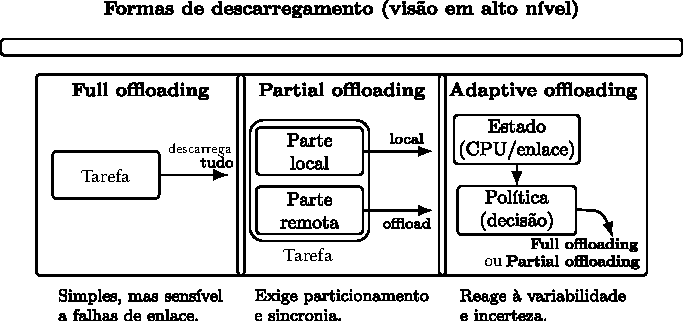
\includegraphics[width=12cm]{figuras/introducao/offloading_categories.pdf}}
    }{
        \Fonte{Elaborado pelo autor}
    }
\end{figure}

Como esquematizado na Figura~\ref{fig:offloading_categories}, o \textit{full offloading} consiste na transferência completa da tarefa da aplicação para um nó remoto, sendo uma estratégia de modelagem simplificada, porém extremamente sensível a falhas de comunicação e à latência da rede. O \textit{partial offloading}, por sua vez, divide a execução do programa entre os recursos locais do veículo e o servidor da rede veicular. Apesar de potencialmente reduzir a sobrecarga de transmissão e o tempo total de resposta, essa abordagem introduz o desafio do particionamento estrutural da tarefa e da sincronização de suas partes. Já o \textit{adaptive offloading} analisa dinamicamente o ambiente para decidir qual a estratégia é mais adequada para cada tarefa, entregando maior resiliência às custas de uma maior complexidade do modelo de tomada de decisão. 

Além disso, as estratégias de decisão variam entre abordagens que processam conjuntos de tarefas em lote (\textit{batch}) ou para cada tarefa, individualmente, direcionando a arquitetura das soluções propostas. A primeira abordagem é mais adequada para aplicações com cargas de trabalho previsíveis e tolerantes a atrasos, como transcodificação de vídeo e processamento de dados em massa~\cite{wang2022}. Nesses cenários, os algoritmos tendem a operar utilizando estatísticas globais para otimizar a alocação de recursos~\cite{li2020genetic, you2021efficient}. Contudo, por assumir parâmetros predeterminados e um ambiente estacionário, essa estratégia tem dificuldades em se adaptar a flutuações repentinas nos cenário observado~\cite{he2025, luo2024}. Em contrapartida, a segunda abordagem, focada na decisão reativa e individual por tarefa, é necessária para sistemas de tempo real e aplicações críticas, como condução autônoma e sensoriamento colaborativo~\cite{RANI2023108543}. Ao processar cada requisição no exato momento de sua chegada, o modelo consegue capturar a imprevisibilidade do ambiente e adaptar o descarregamento de forma contextualizada~\cite{uddin2025}. No entanto, essa abordagem possui uma elevada complexidade de otimização e alocação de recursos~\cite{kandali2025, zhao2025}.

% Avaliar instantaneamente o estado das filas, as restrições de canal e a disponibilidade de nós para cada tarefa isolada gera um severo gargalo computacional, o que justifica a adoção de algoritmos inteligentes e de rápida inferência, como o \gls{DRL}, capazes de balancear latência e energia sem comprometer a estabilidade operacional do sistema~\cite{miriyala2026, uddin2025}.

% Nesse contexto, aplicações com alta demanda computacional e baixa carga de dados (como visão computacional e algoritmos de navegação) impõem restrições de latência que superam a capacidade de processamento das \gls{OBU} locais. Para viabilizar tais aplicações, a tomada de decisão deve integrar, em tempo real, múltiplos indicadores conflitantes (latência, energia, carga de \gls{CPU} e qualidade do canal) sob forte incerteza de medição~\cite{liu2021}. 

Embora a literatura apresente métodos baseados em programação linear, algoritmos gulosos e meta-heurísticas~\cite{li2020genetic,you2021efficient}, tais abordagens operam principalmente sobre instantes isolados da rede (\textit{snapshots}) e assumem decisões de etapa única~\cite{xiang2025}. Essa forma de avaliar o problema pode limitar a eficácia dessas estratégias em cenários veiculares nos quais as métricas variam continuamente (não estacionariedade), pois elas não conseguem capturar o impacto a longo prazo das decisões sequenciais na qualidade de serviço percebida pelos usuários~\cite{uddin2025,cao2024survey}. Para que o descarregamento em redes \gls{V2I}/\gls{V2X} seja de fato confiável e adaptativo, é preciso modelar e lidar diretamente com a incerteza e a variabilidade do ambiente veicular.

Em contrapartida às abordagens tradicionais, as soluções baseadas em \gls{DRL} são capazes de otimizar recompensas sequenciais futuras. No entanto, enfrentam uma limitação estrutural severa, a dependência de um espaço de observação de tamanho fixo~\cite{uddin2025}. Para lidar com variações na quantidade de nós candidatos, a maioria dos modelos recorre a técnicas paliativas que comprometem a escalabilidade~\cite{miriyala2026}. Diante disso, evidencia-se a necessidade de investigar modelos híbridos. A integração de métodos de ranqueamento para filtrar e padronizar as entradas tem o potencial de aprimorar significativamente o processo decisório do \gls{DRL}, superando simultaneamente a inflexibilidade das heurísticas e as limitações estruturais das redes neurais~\cite{vieira2025}.

Adicionalmente, a tomada de decisão nesse ambiente ocorre sob condições de incerteza. Devido à intermitência dos enlaces e à alta latência na sinalização, as informações coletadas sobre a disponibilidade energética ou a carga de processamento dos vizinhos chegam frequentemente ruidosas ou desatualizadas aos agentes de decisão~\cite{uddin2025}. Essa imprecisão e a observabilidade parcial exigem uma avaliação de qualidade dos candidatos que considere a incerteza de forma explícita, buscando garantir a confiabilidade do descarregamento no mundo real~\cite{miriyala2026}. Sob essa ótica, a integração de técnicas que lidam com a incerteza linguística, como a lógica difusa, aos critérios de decisão se mostra promissora para mitigar a variabilidade dos parâmetros e aprimorar o desempenho da arquitetura de descarregamento~\cite{vieira2025, vemireddy2021}.

Outro fator importante diz respeito às tecnologias de comunicação e aos serviços de borda empregados no ambiente veicular. As tecnologias \gls{V2X} e \gls{V2I} viabilizam a troca de dados entre os veículos e a infraestrutura de forma eficiente e em tempo real. Nesse contexto, a arquitetura \gls{VEC} provê aos dispositivos veiculares uma plataforma distribuída para a execução de suas aplicações sensíveis à latência, operando sob a cobertura da rede celular \gls{5G} \gls{NR} para a comunicação com as infraestruturas de borda, e utilizando a interface de comunicação direta \gls{V2X} \textit{Sidelink} para a cooperação entre os veículos vizinhos~\cite{chao2025, luo2024}.


% Os principais desafios inerentes a esse ambiente são sintetizados na Figura~\ref{fig:problems}.

% \begin{figure}[ht!]
%     \centering
%     \Caption{\label{fig:problems}Principais problemas inerentes ao descarregamento de tarefas veicular: mobilidade e instabilidade do enlace, heterogeneidade de recursos e filas, custos energéticos, incerteza de medições, dependência de tecnologias/protocolos e complexidade \textit{NP-hard} sob restrições de latência e confiabilidade.}
%     \UECEfig{}{
%         \fbox{%
%         \resizebox{0.95\linewidth}{!}{%
%         \begin{tikzpicture}[
%           font=\scriptsize\sffamily,
%           node distance=7mm and 9mm,
%           >=Latex
%         ]
%           \tikzset{
%             box/.style={
%               draw, thick, rounded corners=2pt,
%               align=left, inner sep=4pt,
%               text width=3.4cm, minimum height=14mm
%             },
%             cbox/.style={
%               draw, thick, rounded corners=2pt,
%               align=center, inner sep=4pt,
%               text width=3.8cm, minimum height=14mm
%             },
%             arrow/.style={-Latex, thick},
%             group/.style={draw, thick, rounded corners=3pt, inner sep=6pt},
%           }

%           % -----------------------------
%           % Núcleo (centro)
%           % -----------------------------
%           \node[cbox] (decision) {\textbf{Decisão de descarregamento}\\local / MEC / V2V};

%           \node[cbox, above=of decision] (goals)
%             {\textbf{Objetivos / Restrições}\\
%              Reduzir tempo e energia.\\
%              Cumprir restrição de tempo das aplicações.\\
%              Balancear a carga entre os dispositivos.};

%           \node[cbox, above=of goals] (nphard)
%             {\textbf{Complexidade}\\
%              Otimização \textit{NP-hard}\\
%              Exige soluções rápida e adaptativas.};

%           \node[cbox, below=of decision] (model)
%             {\textbf{Modelagem e Protocolos}\\
%              5G NR / \gls{V2X}.\\
%              Descoberta/anúncio de recursos.\\
%              Protocolo para descarregamento.};

%           % -----------------------------
%           % Laterais (problemas do ambiente)
%           % -----------------------------
%           \node[box, left=of decision] (mob)
%             {\textbf{Mobilidade / Canal}\\
%              Flutuação do canal.\\
%              Intermitência na comunicaçao.};

%           \node[box, right=of decision] (hetero)
%             {\textbf{Recursos / Carga}\\
%              CPUs distintas.\\
%              Filas variáveis.\\
%              Balanceamento de carga.};

%           % Contexto acima das laterais (sem aumentar largura)
%           \node[box, above=of mob] (scen)
%             {\textbf{Cenário}\\
%              Urbano ou Rodoviário.\\
%              Densidade e tráfego distintos.};

%           \node[box, above=of hetero] (apps)
%             {\textbf{Aplicações}\\
%              Diferentes perfis e requisitos. 
%              Visão Computacional, Criptografia, Navegação etc.};

%           % Problemas inferiores
%           \node[box, below=of mob] (energy)
%             {\textbf{Energia}\\
%              Custo variável por ciclo.\\
%              Bateria / estado Energético.\\
%              Trade-off energia--tempo};

%           \node[box, below=of hetero] (unc)
%             {\textbf{Incerteza}\\
%              Medições ruidosas.\\
%              Estimativas imperfeitas.\\
%              Estado parcial.};

%           % -----------------------------
%           % Setas (sem cruzamentos)
%           % -----------------------------
%           \draw[arrow] (nphard) -- (goals);
%           \draw[arrow] (goals) -- (decision);

%           \draw[arrow] (model) -- (decision);

%           \draw[arrow] (mob) -- (decision);
%           \draw[arrow] (hetero) -- (decision);

%           \draw[arrow] (energy.north east) -- ($(decision.south west)+(2mm,0mm)$);
%           \draw[arrow] (unc.north west)   -- ($(decision.south east)+(-2mm,0mm)$);

%           \draw[arrow] (scen) -- (mob);
%           \draw[arrow] (apps) -- (hetero);

%           % Moldura (opcional)
%           \begin{pgfonlayer}{background}
%             \node[group, fit=(nphard)(goals)(decision)(model)(scen)(mob)(energy)(apps)(hetero)(unc)] {};
%           \end{pgfonlayer}

%         \end{tikzpicture}%
%         }%
%         }%
%     }{
%         \Fonte{Elaborado pelo autor}
%     }
% \end{figure}


\section{Questões de Pesquisa}
\label{sec:questoes-de-pesquisa}

Este trabalho busca responder às seguintes questões de pesquisa, formuladas a partir das limitações inerentes ao ambiente veicular, da complexidade do problema de descarregamento de tarefas e da necessidade de garantir confiabilidade, eficiência energética e baixa latência em sistemas \gls{VEC}/\gls{V2X}:

\begin{alineas}[label=QP\arabic*.]
    \item \textbf{Como realizar o descarregamento de tarefas em ambientes \gls{V2I}/\gls{V2X} de maneira confiável e adaptativa, considerando a alta variabilidade da mobilidade veicular, da carga computacional e da incerteza nas métricas de decisão?}

    \item \textbf{De que maneira o emprego de modelos híbridos baseados em \gls{DRL} pode aprimorar a qualidade das decisões de descarregamento de tarefas em cenários veiculares altamente dinâmicos, superando as limitações das abordagens determinísticas ou heurísticas?}

    \item \textbf{Em que medida a incorporação da incerteza linguística nos critérios de avaliação dos candidatos ao descarregamento, aprimora a tomada de decisão em cenários de alta mobilidade e informações imprecisas?}
\end{alineas}


\section{Hipóteses}
\label{sec:hipoteses}

A partir das questões acima e da fundamentação teórica apresentada, formulam-se as seguintes hipóteses de pesquisa:

\begin{alineas}[label=H\arabic*.]
    % Como realizar o descarregamento de tarefas em ambientes \gls{V2I}/\gls{V2X} de maneira confiável e adaptativa, considerando a alta variabilidade da mobilidade veicular, da carga computacional e da incerteza nas métricas de decisão?

    \item \textbf{O desenvolvimento de uma política de descarregamento de tarefas que represente o estado do sistema de forma invariante à escala e que considere a incerteza das métricas de decisão viabiliza a criação de um modelo com capacidade de generalização para diferentes cenários de mobilidade e carga de processamento.}

    % De que maneira o emprego de modelos híbridos baseados em \gls{DRL} pode aprimorar a qualidade das decisões de descarregamento de tarefas em cenários veiculares altamente dinâmicos, superando as limitações das abordagens determinísticas ou heurísticas?

    \item \textbf{O uso conjunto de técnicas de avaliação multicritério, focadas no estado imediato do sistema, e de modelos de aprendizado, voltados para a otimização de estados futuros, aprimora a qualidade e a adaptabilidade das decisões de descarregamento frente às limitações das abordagens estritamente determinísticas.}

    % Em que medida a incorporação da incerteza linguística nos critérios de avaliação dos candidatos ao descarregamento, aprimora a tomada de decisão em cenários de alta mobilidade e informações imprecisas?

    \item \textbf{A incorporação da lógica nebulosa nos critérios de avaliação dos candidatos ao descarregamento mitiga o impacto da imprecisão das informações coletadas, conferindo maior robustez e confiabilidade ao processo decisório em cenários de alta mobilidade e incerteza.}


\end{alineas}



\section{Objetivos}
\label{sec:objetivos}

A fim de formalizar o propósito desta pesquisa e as etapas necessárias para sua execução, esta seção detalha os objetivos pretendidos. As metas são apresentadas seguindo uma abordagem \textit{top-down}, partindo de uma visão consolidada da solução proposta até o detalhamento das etapas técnicas e de validação.

\subsection{Objetivo Geral}
\label{sec:objetivo-geral}

Este trabalho tem como objetivo geral desenvolver e avaliar um modelo híbrido de descarregamento de tarefas para redes \gls{VEC}/\gls{V2X}, capaz de garantir confiabilidade e adaptabilidade diante da mobilidade veicular, da variabilidade de carga e da imprecisão de métricas de rede. O modelo integrará métodos de ranqueamento multicritério a algoritmos de \gls{DRL}, gerando um processo decisório estruturado e invariante à escala. Como etapa intermediária, foco deste trabalho, propõe-se validar o acoplamento do ranqueamento multicritério determinístico com o agente de \gls{DRL}. A conclusão do trabalho prevê a extensão deste módulo para incorporar o tratamento de incerteza linguística aos critérios de decisão, culminando na validação da arquitetura completa em um ambiente de simulação.

\subsection{Objetivos Específicos}
\label{sec:objetivos-especificos}


\begin{alineas}[label=OE\arabic*.]
    \item \textbf{Investigar e revisar sistematicamente os modelos de descarregamento de tarefas em cenários \gls{VEC}, identificando as limitações das abordagens tradicionais e os desafios de escalabilidade e engenharia de estado no emprego do \gls{DRL}.}
    \item \textbf{Implementar e validar um módulo de ranqueamento multicritério responsável por pré-avaliar os nós candidatos, abstraindo a variabilidade do ambiente veicular e convertendo o espaço de observação em um vetor compacto, de dimensão fixa e normalizada (etapa intermediária do projeto).}
    \item \textbf{Desenvolver e avaliar uma política de decisão baseada em \gls{DRL} que, ao consumir o estado previamente estruturado pelo ranqueamento, consiga otimizar simultaneamente métricas conflitantes como latência, consumo energético e taxa de cumprimento de prazos (\textit{deadline}).}
    \item \textbf{Aprimorar o módulo de ranqueamento mediante a incorporação de técnicas de modelagem de incerteza (lógica difusa), com o intuito de tolerar ruídos e atrasos nas medições e conferir maior resiliência à etapa de filtragem dos nós candidatos.}
    \item \textbf{Integrar e validar a arquitetura híbrida completa em um simulador de redes de eventos discretos, com modelagem fidedigna de protocolos celulares e interfaces de comunicação veicular direta, conduzindo uma comparação sistemática de desempenho contra abordagens heurísticas e algoritmos do estado da arte.}
\end{alineas}

\section{Contribuições Esperadas}
\label{sec:contribuicoes}
Espera-se que este trabalho produza contribuições relevantes tanto do ponto de vista científico quanto do ponto de vista prático, sobretudo no contexto de sistemas veiculares inteligentes e computação de borda. As principais contribuições previstas são:

\begin{alineas}[label=CE\arabic*.]
\item \textbf{Proposição de uma arquitetura de decisão híbrida que acopla métodos de ranqueamento multicritério a um modelo de \gls{DRL}, demonstrando a capacidade de tomada de decisão adaptativa e de generalização estrutural para cenários com variadas densidades de tráfego veicular.}.

\item \textbf{Desenvolvimento e validação de módulos de ranqueamento que atuam simultaneamente como redutores de dimensionalidade do estado e como filtros de incerteza linguística, viabilizando o tratamento de informações ruidosas e atrasadas para aumentar a confiabilidade da seleção de nós candidatos.}.

\item \textbf{Construção e integração de modelos de avaliação em plataformas de simulação de rede, englobando aspectos realistas de mobilidade, heterogeneidade computacional e protocolos de comunicação celular e veicular direta (\textit{sidelink}), estabelecendo um ambiente fidedigno para testes de arquiteturas \gls{VEC}.}

\item \textbf{Avaliação extensiva e comparação sistemática do modelo híbrido proposto contra métodos heurísticos e abordagens puramente baseadas em \gls{DRL}, evidenciando os ganhos em métricas de desempenho críticas, tais como redução de latência, eficiência energética e taxa de atendimento a prazos (\textit{deadlines}).}

\item \textbf{Consolidação de um conjunto de diretrizes práticas para o projeto de sistemas de descarregamento em arquiteturas de borda veicular, orientando pesquisadores e engenheiros sobre a aplicação de métodos híbridos.}

\end{alineas}

\section{Publicação}
\label{sec:publicacao}

Como parte do desenvolvimento deste trabalho, foi submetido e aceito um artigo no periódico internacional \textit{Cluster Computing} (Springer), classificado como Q1 nas bases \textit{Scopus/SJR} e posicionado no percentil superior da área de \textit{Computer Networks and Communications}. O artigo, intitulado ``\textit{FOFF: an energy-efficient task offloading in VEC-enabled vehicular networks using fuzzy TOPSIS}''~\cite{vieira2025}, apresenta uma versão preliminar do modelo híbrido de descarregamento de tarefas proposto neste trabalho, incluindo a arquitetura conceitual e os primeiros resultados derivados de experimentos em simulação. A publicação serviu tanto como validação da relevância científica da abordagem quanto como etapa intermediária para o refinamento metodológico, a ampliação dos cenários simulados e o aprofundamento das análises apresentadas nos capítulos seguintes.

\section{Organização do Trabalho}
\label{sec:organizacao}

Este documento está estruturado partindo dos fundamentos teóricos até o delineamento da solução proposta e o planejamento para a finalização da pesquisa. A organização segue o seguinte formato:

\begin{itemize}
    % \item \textbf{Capítulo~\ref{cap:introducao} --- Introdução:} apresenta o contexto geral, a motivação, a definição do problema, as questões de pesquisa, hipóteses e objetivos, além das contribuições esperadas e publicações decorrentes.

    \item \textbf{Capítulo~\ref{cap:fundamentacao-teorica} --- Fundamentação Teórica:} discute os conceitos essenciais que sustentam este trabalho, abrangendo arquiteturas \gls{5G} \gls{NR} e \textit{Sidelink} \gls{V2X}, o paradigma de descarregamento de tarefas em ambientes \gls{VEC}, fundamentos de \gls{DRL} e o método de decisão multicritério \gls{TOPSIS} com sua extensão \textit{Fuzzy}-\gls{TOPSIS}.

    \item \textbf{Capítulo~\ref{cap:revisao-literatura} --- Revisão da Literatura:} realiza uma análise crítica de trabalhos recentes, explorando as principais técnicas e tendências voltadas ao descarregamento de tarefas em cenários veiculares altamente dinâmicos.

    \item \textbf{Capítulo~\ref{chap:proposta} --- Proposta:} detalha a arquitetura \gls{SAC}-\gls{TOPSIS} desenvolvida como etapa intermediária desta qualificação, descrevendo a integração entre o algoritmo Soft \textit{Actor}-\textit{Critic} e o ranqueamento multicritério, bem como a modelagem do ambiente de simulação e os resultados experimentais obtidos.

    \item \textbf{Capítulo~\ref{chap:conclusoes} --- Conclusão:} sintetiza as principais descobertas desta etapa de qualificação, discute as limitações atuais e aponta os próximos passos para a validação final do modelo.

    \item \textbf{Capítulo~\ref{cap:cronograma-pesquisa} --- Cronograma:} descreve o planejamento das atividades futuras para a conclusão do doutorado, estabelecendo os prazos para experimentos finais, redação da tese e defesa.

    \item \textbf{Apêndice~\ref{ap:conversao-alibaba} --- Conversão de Escala do \textit{Trace} Alibaba:} descreve o procedimento de conversão do \textit{trace} de carga de trabalho real do Alibaba para o contexto do cenário veicular simulado, detalhando os fatores de escala temporal adotados.
\end{itemize}
	\input{elementos-textuais/fundamentacao-teorica}
	% \chapter{Trabalhos Relacionados}
\label{cap:trabalhos-relacionados}

Integer non lacinia magna. Aenean tempor lorem tellus, non sodales nisl commodo ut. Proin mattis placerat risus sit amet laoreet. Praesent sapien arcu, maximus ac fringilla efficitur, vulputate faucibus sem. Donec aliquet velit eros, sit amet elementum dolor pharetra eget. Integer eget mattis libero

\section{Revisão da Literatura}
\label{sec:revisao-literatura}

\section{Trabalho Relacionados}
\label{sec:trabalho-relacionado-a}

O problema de descarregamento de tarefas em \gls{VEC} tem sido extensivamente estudado. Abordagens baseadas em \gls{DRL}, como a proposta por~\citeonline{shi2023}, demonstram sucesso na otimização de decisões de descarregamento, obtendo reduções significativas no tempo de resposta e consumo energético. No entanto, esses modelos podem enfrentar instabilidade quando o estado do ambiente (ex: qualidade do canal, carga do servidor) é volátil e difícil de modelar deterministicamente.

Paralelamente, a Lógica \textit{\textit{Fuzzy}} é reconhecida por sua capacidade de lidar com incerteza. Trabalhos como o de~\citeonline{gao2022fuzzy} utilizam inferência \textit{\textit{fuzzy}} para balanceamento de carga em redes heterogêneas, e~\citeonline{kousar2025fuzzy} aplicam otimização \textit{\textit{fuzzy}} em problemas multiobjetivo complexos. Essas abordagens, embora robustas à incerteza, geralmente carecem de adaptabilidade em tempo real, pois suas regras são muitas vezes estáticas.

Para unir o melhor de ambas as abordagens, propõe-se a integração de Lógica \textit{\textit{Fuzzy}} com \gls{DRL}. A inspiração metodológica central vem de~\citeonline{rezaei2025integrating}, que, embora focado no mercado financeiro, demonstra como indicadores \textit{\textit{fuzzy}} podem aprimorar a entrada de um agente \gls{DRL}, estabilizando o aprendizado em ambientes não estacionários. Esta metodologia tem sido adaptada com sucesso para o contexto de \gls{VEC}.~\citeonline{zhang2023fuzzy_drl_offloading} e~\citeonline{li2024hybrid_fuzzy_drl_v2x} utilizam sistemas \textit{\textit{fuzzy}} para pré-processar o estado da rede (mobilidade, qualidade do link) antes de alimentar um agente \gls{DRL}, resultando em políticas de descarregamento mais eficientes. Outras abordagens, como a de~\citeonline{chen2022fuzzy_dqn_vec}, exploram a fusão das técnicas na própria arquitetura do \gls{DRL}, como em \textit{Fuzzy Deep Q-Networks}.

Este artigo introduz o ANS-\gls{V2X}, uma estrutura de seleção de rede adaptativa focada em sistemas \gls{V2X} que operam sob densidades veiculares variáveis e condições de redes heterogêneas. Com a demanda por comunicações de baixa latência e alta taxa de transferência, o \textit{framework} integra diversas Tecnologias de Acesso de Rádio (RATs), como \gls{DSRC}, \gls{LTE} e \gls{5G} \gls{NR}. Através de uma abordagem baseada em heurística, o modelo aloca veículos às redes levando em consideração a sensibilidade da aplicação (como segurança versus infoentretenimento), além de restrições de latência, carga computacional e direcionalidade~\cite{haq2025}.

A avaliação da estrutura proposta é realizada através de um \textit{benchmark} contra métodos de Programação Linear Inteira Mista (MILP) e abordagens baseadas em \textit{\textit{Q-learning}}. Os resultados das simulações demonstram que o ANS-\gls{V2X} atinge um desempenho quase ideal (geralmente entre 5\% e 10\% da utilidade do MILP) com a grande vantagem de reduzir o tempo de execução de decisões em mais de 85\%, completando a seleção em menos de 15 milissegundos. Isso confirma a viabilidade de sua implantação em borda para aplicações em tempo real~\cite{haq2025}.


O estudo aborda o problema de descarregamento de tarefas em redes veiculares assistidas por \gls{MEC}. Os autores formulam um modelo de otimização multiobjetivo focado no veículo (MOTO), cujo propósito é minimizar o tempo médio de atraso, o consumo de energia e os custos de pagamento para os veículos autônomos conectados (CAVs). Para isso, a pesquisa emprega a teoria das filas (como M/M/1 e M/M/c) para modelar os tempos de processamento e os processos de espera durante o processamento local e de descarregamento~\cite{chen2025}.

Como solução, é proposta uma abordagem em duas etapas. Primeiramente, aplica-se uma estratégia de triagem de tarefas baseada na urgência e criticidade (utilizando o método \gls{TOPSIS} ponderado por entropia) para tomar decisões rápidas em tarefas com características extremas. Na segunda etapa, um \textit{framework} multiobjetivo baseado em Entropia Máxima Bayesiana (BME) associado a um algoritmo genético híbrido (MO-HGA) lida com o problema restante. Testes extensivos utilizando dados reais da cidade de Wuhan mostram que o sistema supera seis outros algoritmos multiobjetivos de ponta~\cite{chen2025}.

O artigo propõe uma solução robusta para o descarregamento de tarefas de segmentação de imagem e alocação de recursos em cenários de \gls{IoV}. Para mitigar as limitações computacionais dos veículos inteligentes, os pesquisadores projetaram um sistema eficiente apoiado por um algoritmo \textit{model-free} melhorado chamado PER-iSAC, que baseia-se na arquitetura Soft \textit{Actor}-\textit{Critic} (\gls{SAC}) e é aprimorado com a técnica de \textit{Prioritized Experience Replay} (PER)~\cite{zou2025}.

A principal inovação do PER-iSAC está na capacidade de acelerar o aprendizado, manter a estabilidade em cenários dinâmicos e melhorar drasticamente a precisão da alocação das tarefas entre os servidores de borda (edge servers). Experimentos de simulação mostram que o PER-iSAC supera algoritmos de referência tradicionais (como \gls{PPO} e \gls{SAC} padrão), reduzindo de maneira significativa tanto as taxas de erro nas decisões de alocação quanto os tempos gerais de conclusão das tarefas computacionais intensivas~\cite{zou2025}.

Nesta pesquisa, é atacado o problema de desequilíbrio de carga nos servidores de borda veicular (\gls{MEC}) gerado pela distribuição não uniforme de veículos transferindo dados simultaneamente. O artigo formula uma estratégia que considera o descarregamento parcial de tarefas (descarregamento parcial) e as flutuações de carga na borda para minimizar o custo geral do sistema, modelando a interação veículo-\gls{MEC} via \gls{MDP}~\cite{wu2024}.

Para obter as decisões ótimas de descarregamento e alocação de recursos, os autores utilizam o algoritmo \gls{TD3}. Visando alcançar o balanceamento da carga, a colaboração entre os servidores de borda é incorporada utilizando a técnica multicritério \gls{TOPSIS} para a seleção adequada do servidor. O método proposto demonstra ser capaz de otimizar significativamente a utilização dos recursos do sistema, provando-se superior na redução de latência e consumo de energia quando comparado a soluções de \textit{baseline} convencionais~\cite{wu2024}.

Este trabalho de pesquisa introduz um modelo preditivo híbrido voltado para o mercado financeiro, combinando Decomposição Modal Empírica de Conjunto Completo com Ruído Adaptativo (CEEMDAN) e memória de longo e curto prazo (\gls{LSTM}). O foco é prever a volatilidade realizada (RV) de índices de preços de ações (como o CSI300, S\&P500 e STOXX50). O CEEMDAN atua primeiro reduzindo o ruído e extraindo componentes intrínsecos da série temporal altamente ruidosa antes de fornecê-los à rede \gls{LSTM}~\cite{lin2022}.

As avaliações do modelo foram feitas utilizando quatro funções de perda distintas (MSE, MAE, HMSE, HMAE) e o teste estatístico \textit{Model Confidence Set} (MCS). O modelo proposto (CEEMDAN-LSTM) superou de forma contundente os modelos únicos concorrentes (como BP, ELMAN, SVR, HAR e \gls{AR}), confirmando a hipótese de que a abordagem híbrida é muito mais eficaz na captura de tendências e características não lineares tanto em mercados emergentes quanto em mercados desenvolvidos~\cite{lin2022}.

O artigo aborda as adversidades encontradas por sistemas embarcados em veículos modernos que precisam processar uma crescente variedade de aplicações com eficácia, apesar da instabilidade das redes de comunicação. O modelo proposto implanta \gls{VEC} através da introdução de um algoritmo inteligente suportado por Aprendizado por Reforço Profundo Multiagente (MADRL) conjugado com um jogo de Stackelberg de quatro etapas~\cite{fofana2024}.

Neste \textit{framework}, os recursos são provisionados tanto pelas \gls{RSU} quanto por "veículos de serviço" ociosos. Através do jogo de Stackelberg, a estratégia alcança um Equilíbrio de Nash estável que rege a tarifação e a compra de capacidade computacional. Os resultados comprovam que a arquitetura otimiza tempo, despesas e a utilidade mútua de todos os agentes do sistema, aumentando a probabilidade de êxito na execução de tarefas em relação a soluções competidoras como o MADQN~\cite{fofana2024}.

Este trabalho inova ao focar nas áreas simultâneas de segurança, custo e gestão de energia em sistemas de Internet de Veículos assistidos por \gls{MEC} (\gls{IoV}-\gls{MEC}). Os autores aplicam a arquitetura \gls{DDQN} combinada com a tecnologia Blockchain. O papel da Blockchain aqui é prover segurança e descentralização para a proteção e integridade da comunicação, enquanto o algoritmo \gls{DDQN} atua na tomada de decisão em tempo real~\cite{moghaddasi2024}.

A modelagem multiobjetivo faz uma gestão avançada de trade-offs de diversos parâmetros, balanceando com precisão os tempos de resposta, a vida útil de energia e as despesas computacionais e de comunicação no cenário veicular dinâmico. As simulações apontaram que o \gls{DDQN} foi capaz de reduzir o consumo de energia em cerca de 26,4\%, a latência em 6,87\% e o custo total do sistema em 7,41\% quando confrontado com algoritmos como \gls{DQN} e \gls{DDPG}~\cite{moghaddasi2024}.

Visando o rigoroso contexto da tecnologia espacial, o estudo em questão propõe um modelo TCN-\gls{TOPSIS} destinado a monitorar o status de segurança de voos de foguetes operando em um sistema de Gêmeos Digitais (Digital Twin). A Rede Convolucional Temporal (TCN) é aplicada devido ao seu poder de processar modelos de sequências complexas temporalmente, capturando informações sem as severas penalidades de latência computacional sofridas pelas redes \gls{RNN} tradicionais~\cite{li_fugang_2025}.

Subsequentemente, a metodologia \gls{TOPSIS} é adotada para agregar e avaliar os múltiplos parâmetros críticos de voo preditos em tempo real. O sistema demonstrou excelência empírica, provando ser capaz de predizer o status de segurança do foguete em menos de 3 milissegundos. Tais características colocam a abordagem acima de arquiteturas \gls{RNN}, GRU e \gls{LSTM}, mostrando grande capacidade como ferramenta de suporte à decisão preventiva e destrutiva emergencial durante missões de lançamento de foguetes~\cite{li_fugang_2025}.

Este artigo introduz uma abordagem de \textit{software} baseada em \gls{IA} generativa para revolucionar o método de seleção de pessoal na área de engenharia de \textit{software}. Combinando Processamento de Linguagem Natural (NLP) por meio de \glspl{LLM} refinados (especificamente o DistilRoBERTa) e a teoria multicritério \textit{\textit{Fuzzy}} \gls{TOPSIS}, os autores extraem, classificam e pontuam candidatos a partir de dados coletados da plataforma LinkedIn (como Experiência, Educação, Habilidades e o "Sobre")~\cite{hoque2024}.

A utilização dos números \textit{\textit{fuzzy}} triangulares (TFNs) no modelo \gls{TOPSIS} resolve a problemática da ambiguidade e subjetividade inerentes às avaliações realizadas por humanos. Os resultados empíricos da predição baseada no modelo LLM-\textit{\textit{Fuzzy}} \gls{TOPSIS} apresentaram uma concordância acentuada com os especialistas em recursos humanos, atingindo mais de 91\% de acurácia no processo de classificação, oferecendo desta forma uma solução automatizada, imparcial e escalável para o recrutamento e ranqueamento de talentos~\cite{hoque2024}.

O décimo estudo centra-se na dificuldade em aliviar cargas de trabalho originadas de veículos mecânicos num ambiente veicular de borda dinâmico com recursos limitados. Para responder a essas variáveis de rede em constante evolução, o documento propõe o emprego do modelo \textit{Variational Autoencoders} atrelado à rede \textit{Long Short-Term Memory} (VAE-LSTM) para decisões precisas de descarregamento~\cite{xiang2026}.

Neste conjunto, a capacidade generativa do VAE opera em sinergia perfeita com o mapeamento e análise de tendências de séries temporais do \gls{LSTM}, lidando eficientemente com as mudanças rápidas e incertas dos estados da rede e do ambiente. As avaliações simuladas atestaram que o VAE-LSTM supera os modelos \gls{GAN}, CNN e \gls{RNN}, tanto na taxa de sucesso da transferência das tarefas quanto na diminuição drástica do erro médio absoluto, assegurando assim alta confiabilidade e latência mínima para sistemas de Internet de Veículos (\gls{IoV})~\cite{xiang2026}.


% \section{Trabalho Relacionado B}
% \label{sec:trabalho-relacionado-b}

% Integer non lacinia magna. Aenean tempor lorem tellus, non sodales nisl commodo ut. Proin mattis placerat risus sit amet laoreet. Praesent sapien arcu, maximus ac fringilla efficitur, vulputate faucibus sem. Donec aliquet velit eros, sit amet elementum dolor pharetra eget. Integer eget mattis libero. Praesent ex velit, pulvinar at massa vel, fermentum dictum mauris. Ut feugiat accumsan augue, et ultrices ipsum euismod vitae

% 	\begin{figure}[ht!]
% 		\centering
% 		\Caption{\label{fig:exemplo-4} Maecenas luctus augue odio, sed tincidunt nunc posuere nec}	
% 		\UECEfig{}{
% 			\fbox{
\includegraphics[width=8cm]{figuras/figura-4}}
% 		}{
% 			\Fonte{Elaborado pelo autor}			
% 		}	
% 	\end{figure}

% Nunc ac pretium dui. Mauris aliquam dapibus nulla ac mattis. Aenean non tortor volutpat, varius lectus vitae, accumsan nibh. Cras pretium vestibulum enim, id ullamcorper tortor ultrices non. Integer sodales viverra faucibus. Curabitur at dui lacinia, rhoncus lacus at, blandit metus. Integer scelerisque non enim quis ornare.

% 	\begin{quadro}[ht!]	
% 		\centering
% 		\Caption{\label{qua:exemplo-1} Praesent ex velit, pulvinar at massa vel, fermentum dictum mauris. Ut feugiat accumsan augue}		
% 		\UECEqua{}{
% 			\begin{tabular}{|c|c|l|l|}
% 				\hline
% 				Quisque & pharetra & tempus & vulputate \\
% 				\hline
% 				E1 & Complete coverage by a single transcript & Both  & Complete\\
% 				\hline
% 				E2 & Complete coverage by more than & Both splice sites & Complete\\
% 				\hline
% 				E3 & Partial coverage & Both splice sites & Both \\				
% 				\hline
% 			\end{tabular}
% 		}{
% 			\Fonte{Elaborado pelo autor}
% 		}
% 	\end{quadro}
	
% Donec luctus nunc eget mi pellentesque, ac finibus orci placerat. Aenean vestibulum odio at neque tempor convallis. Maecenas elit magna, fringilla consequat lorem id, faucibus dictum turpis. Fusce vel suscipit nunc. Morbi facilisis odio in turpis gravida, eu porta metus ultricies. Sed tincidunt eget nulla eget tempor. Fusce orci velit, posuere in scelerisque a, vehicula sed leo. Phasellus sagittis, mauris id iaculis vehicula, enim diam faucibus nisi, vel condimentum lectus urna id eros. Morbi et ante ligula. Nullam eu dolor eget diam consectetur faucibus eget et lorem. Nam tempor, arcu ut fringilla scelerisque, diam risus molestie metus, ac condimentum nisl diam eu tortor. Aliquam fringilla commodo libero, et mollis mi varius id. Etiam vel vehicula sapien. Cras volutpat eros vehicula, vehicula ex non, sagittis purus. Phasellus pellentesque lacus semper, egestas ante eu, molestie massa. Fusce dictum non justo id viverra.

	
% 	\begin{quadro}[ht!]	
% 		\centering
% 		\Caption{\label{qua:exemplo-2} Duis faucibus, enim quis tincidunt pellentesque}		
% 		\UECEqua{}{
% 			\begin{tabular}{|c|c|}
% 				\hline
% 				Quisque & pharetra \\
% 				\hline
% 				E1 & Complete coverage by a single transcript \\
% 				\hline
% 				E2 & Complete coverage by more than \\
% 				\hline
% 				E3 & Partial coverage \\
% 				\hline
% 				E4 & Partial coverage \\
% 				\hline
% 				E5 & Partial coverage \\
% 				\hline
% 				E6 & Partial coverage \\
% 				\hline
% 				E7 & Partial coverage \\
% 				\hline
% 			\end{tabular}
% 		}{
% 			\Fonte{Elaborado pelo autor}
% 		}
% 	\end{quadro}

% Mauris laoreet, turpis et congue mollis, nibh felis mollis ante, a malesuada sapien mauris nec sem. Phasellus nec orci euismod purus auctor viverra auctor vitae nibh. Donec laoreet ante leo, a accumsan dolor convallis et. Donec rutrum nisl ut odio dignissim molestie. Pellentesque vitae diam gravida, convallis nisi sed, dapibus eros. Aliquam consectetur sed nibh vitae rhoncus. In sed ipsum lacus. Suspendisse nulla mi, convallis in arcu eget, consectetur euismod arcu. Maecenas eu tincidunt nisl, non finibus dui. Aliquam lorem lacus, pellentesque in metus eu, placerat ullamcorper metus. Sed condimentum cursus accumsan. Nullam a elementum ex.

% Integer non lacinia magna. Aenean tempor lorem tellus, non sodales nisl commodo ut. Proin mattis placerat risus sit amet laoreet. Praesent sapien arcu, maximus ac fringilla efficitur, vulputate faucibus sem. Donec aliquet velit eros, sit amet elementum dolor pharetra eget. Integer eget mattis libero.
% \Gls{ambiguidade}
% \Gls{braile}
% \Gls{coerencia}
% \Gls{dialetos}
% \Gls{elipse}
% \Gls{locucao-adjetiva}
% \Gls{modificadores}
% \Gls{paronimos}
% \Gls{sintese}
% \Gls{borboleta}
	\chapter{Revisão de Literatura  }
\label{cap:revisao-literatura}

% \section{Aplicações em Redes Veiculares}
% \label{sec:aplicacoes-em-redes-veiculares}

% \section{Técnicas de Offloading em Ambientes Veiculares}
% \label{sec:tecnicas-de-offloading-em-ambientes-veiculares}

% \section{Modelos Híbridos Fuzzy e Aprendizado por Reforço}
% \label{sec:modelos-hibridos-fuzzy-e-aprendizado-por-reforco}

% \section{Problemas e Desafios Atuais}
% \label{sec:problemas-e-desafios-atuais}

Este capítulo apresenta uma análise crítica e comparativa dos trabalhos mais recentes e relevantes para o desenvolvimento desta proposta. A literatura é organizada segundo uma taxonomia adaptada de~\cite{de2020computation}, estruturada em duas vertentes. A Seção~\ref{sec:padrao-comunicacao} examina o Padrão de Comunicação adotado pelos trabalhos relacionados, considerando as tecnologias de rede empregadas e os servidores de borda utilizados; e a Seção~\ref{sec:problema} analisa a Formulação do Problema de descarregamento, com ênfase nas estratégias baseadas em \gls{DRL}, na engenharia de estado e recompensa, e nos ambientes de simulação adotados. Por fim, a Seção~\ref{sec:consideracoes-finais-revisao} sintetiza as lacunas identificadas e posiciona a contribuição desta proposta frente ao estado da arte.

\section*{Taxonomia}

Para classificar e relacionar o estado da arte das soluções de descarregamento de tarefas em ambientes de \gls{VEC}, adotou-se uma versão adaptada da taxonomia proposta em~\cite{de2020computation}, sendo ela dividida em duas vertentes estruturais: Padrão de Comunicação, que avalia as tecnologias de rede e os servidores utilizados; e Problema, que analisa as estratégias com ênfase em modelos \gls{DRL}. Dessa maneira, os artigos relacionados foram classificados conforme a Figura~\ref{fig:taxonomia_adaptada}.

\begin{figure}[ht!]
\centering
\resizebox{\linewidth}{!}{%
\begin{forest}
  for tree={
    font=\sffamily\normalsize,
    draw=teal!80!black,
    very thick,
    rounded corners=4pt,
    fill=teal!70!black,
    text=white,
    align=center,
    edge={draw=teal!60!black, thick},
    l sep=6mm,
    s sep=2mm,
    if level=0{
      minimum height=8mm,
      font=\sffamily\normalsize\bfseries,
    }{
      if level=1{
        fill=teal!60!black,
        font=\sffamily\normalsize\bfseries,
        minimum height=7mm,
      }{
        if level=2{
          fill=teal!50!black,
          font=\sffamily\normalsize\bfseries,
          minimum height=6mm,
        }{
          % Leaf nodes
          fill=teal!40!black,
          font=\sffamily\normalsize,
          draw=teal!50!black,
          rounded corners=3pt,
          align=left,
          inner sep=2pt,
          thin,
        }
      }
    }
  }
  [Descarregamento\\Computacional Veicular
    [Padrão de\\Comunicação
      [Tecnologia
        [{$\triangleright$ C-\gls{V2I} / C-\gls{V2X}\\$\triangleright$ 5G / 6G}]
      ]
      [Servidor
        [{$\triangleright$ \gls{MEC} (Borda Fixa)\\$\triangleright$ Nuvens Veiculares\\$\triangleright$ Nuvem}]
      ]
    ]
    [Problema
      [Estratégia
        [Função Objetivo
          [{$-$ Tempo de\\~~~Resposta\\$-$ Consumo\\~~~Energético\\$-$ Custos Financeiros\\$+$ Estabilidade de\\~~~Filas (Lyapunov)\\$+$ Taxa de Sucesso\\$+$ Nível de Confiança}]
        ]
        [Eng. de Estado
          [{$\triangleright$ Tamanho das Filas\\$\triangleright$ Prioridade / \textit{Deadline}\\$\triangleright$ Escores de Confiança\\$\triangleright$ Ângulos e Orientação}]
        ]
        [Eng. de Recompensa
          [{$\triangleright$ Pesos Dinâmicos\\$\triangleright$ Penalização Severa\\$\triangleright$ Recompensa Global\\$\triangleright$ Estágios Sequenciais\\$\triangleright$ Drift-plus-penalty}]
        ]
        [Modelos
          [{$\triangleright$ \gls{DQN}, D3QN, P-\gls{DQN}\\$\triangleright$ \gls{SAC}, DDPG, QDPG\\$\triangleright$ L-MADDPG, SIDDPG\\$\triangleright$ Fusões: FL, DT, GNN}]
        ]
      ]
      [Ambiente\\Simulado
        [{$\triangleright$ Mobilidade: SUMO,\\~~~PTV Vissim\\$\triangleright$ Rede: ns-3\\$\triangleright$ Agente: OpenAI Gym\\$\triangleright$ Dados Reais (Traces)}]
      ]
    ]
  ]
\end{forest}
}
\Caption{\label{fig:taxonomia_adaptada} Taxonomia adaptada para classificação dos trabalhos relacionados em descarregamento computacional veicular, com ênfase na modelagem de \gls{DRL} e ambiente de simulação.}
\Fonte{Adaptado de~\citeonline{de2020computation}.}
\end{figure}

\section{Padrão de Comunicação}
\label{sec:padrao-comunicacao}
No descarregamento de tarefas, o cenário de comunicação celular vem ganhando bastante destaque. Neste quesito, suas tecnologias vêm evoluindo rapidamente e ditam a maioria das pesquisas aqui apresentadas. A seguir são apresentados alguns trabalhos que utilizam tecnologias \gls{5G} e além (\gls{B5G}/\gls{6G}) para atender às exigentes demandas relacionadas a aplicações veiculares.

\subsection{Tecnologia}
A evolução das tecnologias de comunicação veicular destaca a transição de padrões tradicionais, como o \gls{DSRC} e o IEEE 802.11bd, para a comunicação celular aliada à \gls{IA}. Essa mudança visa, sobretudo, possibilitar baixas latências e alta vazão de dados em cenários de alta mobilidade, contribuindo para resolver o problema de descarregamento de tarefas. Nesse contexto, diversos trabalhos, como os de~\cite{Moghaddasi2023, sidwini, li2025, meghamala2025}, utilizam interfaces \gls{C-V2X} e arquiteturas de borda para o compartilhamento de informações em aplicações veiculares avançadas. 

O estudo de~\cite{Moghaddasi2023} propõe um algoritmo de \gls{DRL}, especificamente o \gls{DDQN}, em redes \gls{5G} para solucionar o problema de descarregamento de tarefas utilizando a comunicação \gls{V2I} para alcançar eficiência energética e a diminuição da latência. O trabalho de~\cite{sidwini} explora o uso de algoritmos avançados de \gls{DRL}, como o \gls{SAC}, para otimizar o descarregamento dinâmico entre dispositivos locais, servidores de borda e a nuvem, equilibrando o consumo de energia e o atraso na execução. Em um cenário direcionado aos sistemas \gls{6G},~\cite{li2025} introduz um esquema inteligente baseado em \gls{DQN} em redes \gls{V2X} assistidas por \gls{MEC} para otimizar conjuntamente a associação aos servidores, a taxa de descarregamento de tarefas e a aceleração dos veículos. Essa abordagem visa minimizar o atraso do sistema e evitar colisões de trânsito, utilizando uma função de recompensa segmentada que respeita restrições de atraso, energia e segurança. Por fim,~\cite{meghamala2025} propõe um \textit{framework} de \gls{MARL} para redes \gls{5G} que combina o algoritmo \gls{SAC} com arquiteturas hierárquicas (\gls{MATD3} e \gls{TD2PG}). Essa solução visa a alocação dinâmica de subcanais, potência de transmissão e recursos computacionais em servidores \gls{MEC}, levando em consideração a mobilidade dos usuários e o isolamento das fatias de rede (\textit{network slicing}).

\subsection{Servidor}
O \gls{VEC} é um paradigma amplo que integra dois ambientes complementares de execução remota: a infraestrutura de borda fixa, composta por servidores \gls{MEC} acoplados a \glspl{RSU} ou estações base e acessíveis via comunicação \gls{V2I}; e as Nuvens Veiculares, formadas pelos recursos computacionais ociosos dos próprios veículos e acessíveis por meio de canais diretos \gls{V2V}. Esses dois ambientes podem operar de forma isolada ou integrada. Adicionalmente, quando as restrições de latência permitem, tarefas podem ser delegadas a uma infraestrutura de nuvem remota, que oferece maior capacidade de processamento ao custo de latência consideravelmente superior. A seguir, são descritas as abordagens modeladas para cada um desses ambientes de execução nos trabalhos relacionados.

\section*{\texorpdfstring{\gls{MEC}}{\gls{MEC}}}
Servidores \gls{MEC} contribuem significativamente para atender exigências de \gls{URLLC} em \gls{5G} \gls{NR}. Eles ficam localizados na borda da rede e podem ser constituídos de equipamentos robustos, capazes de auxiliar no processamento pesado de tarefas delegadas por outros dispositivos com recursos limitados.

Nesse contexto, esses servidores frequentemente estão conectados a \gls{RSU} e estações base para oferecer suporte computacional de baixa latência aos veículos. Aproveitando essa infraestrutura de borda, o estudo de~\cite{zhao2025} propõe o esquema \gls{PDQKM} para otimizar o descarregamento de múltiplas tarefas, permitindo reduzir a latência total do sistema. Por outro lado, o trabalho de~\cite{wu2025} utiliza \gls{GAN} para expandir amostras de tarefas evitando o desequilíbrio de dados, criando um modelo de \gls{FL} para realizar o descarregamento de tarefas de forma energeticamente eficiente em servidores \gls{MEC}. O estudo de~\cite{mohammad2025} apresenta o \textit{framework} EMEC-IoVTOF, que integra \gls{DRL} com a técnica de \gls{PSO} para otimizar a alocação de recursos em sistemas \gls{IoV}. A solução calcula custos de descarregamento para evitar a convergência para ótimos locais, conseguindo reduções significativas de latência e consumo de energia, além de contornar restrições de largura de banda em cenários veiculares dinâmicos. Por sua vez, o estudo de~\cite{liu2025} utiliza o método de aproximação de Bernstein para converter restrições probabilísticas de interferência em formato tratável, minimizando uma função de utilidade que equilibra atrasos na transmissão e na computação para o \gls{C-MEC}.

Nessa mesma direção, o trabalho de~\cite{vieira2025} propõe a política de descarregamento de tarefas \gls{FOFF}, voltada para redes \gls{VEC} habilitadas por \gls{5G} via comunicação \gls{V2I}. Em vez de recorrer a técnicas iterativas de aprendizado, o FOFF emprega o método de \gls{MCDM} \textit{Fuzzy}-\gls{TOPSIS} com Números Fuzzy Triangulares (TFNs) para capturar a incerteza e a variabilidade dos recursos dos servidores \gls{MEC} em tempo de decisão, sem a necessidade de uma fase de treinamento prévio. A política resultante determina, para cada tarefa gerada pelo veículo, se o processamento deve ocorrer localmente na \gls{OBU} ou ser descarregado para o servidor de borda fixo, com base na pontuação de proximidade relativa calculada pelo \textit{Fuzzy}-\gls{TOPSIS} em função do tempo de resposta e do consumo energético. Avaliado em um simulador com heterogeneidade computacional, o \gls{FOFF} demonstrou superioridade sobre métodos gulosos (GTT), heurísticas particionadas (FP-Sched) e abordagens baseadas em algoritmos genéticos (HOFF), alcançando reduções no consumo energético de até 72,11\%.

\section*{Nuvens Veiculares}

As Nuvens Veiculares constituem o ambiente de execução cooperativo do paradigma \gls{VEC} baseado em comunicação \gls{V2V}. Nesse ambiente, os recursos computacionais ociosos das unidades embarcadas (\gls{OBU}) dos próprios veículos são disponibilizados para auxiliar nós vizinhos por meio de canais de comunicação direta, sem necessidade de intermediação por infraestruturas estáticas da pista. O estudo de~\cite{xie2025} propõe utilizar \gls{RIS} juntamente com \gls{VEC} para reduzir custos de implantação, ao mesmo tempo que busca maximizar \gls{SOE} via algoritmo \gls{PPO}, otimizando conjuntamente decisões de descarregamento, alocação de recursos computacionais e vetores de mudança de fase. Por sua vez,~\cite{wu2025ava} utiliza \gls{FL} e \gls{MADDPG}, empregando mecanismos de incentivo baseados em reputação para determinar a proporção ideal de recursos cedidos por veículos vizinhos, visando minimizar latência e consumo de energia e garantindo alta taxa de conclusão em tarefas computacionalmente intensivas. O trabalho de~\cite{long2025} desenvolve o algoritmo \gls{CTSRAO}, que integra dispositivos finais, borda veicular e nuvem para realizar descarregamento parcial de tarefas, separando o problema em subproblemas convexos para otimizar de forma colaborativa o \textit{task splitting} (taxa de divisão de tarefas) e a alocação de recursos computacionais, alcançando equilíbrio de desempenho global do sistema. Em~\cite{abbas2025}, propõe-se um algoritmo baseado em aprendizado descentralizado colaborativo, que orquestra a execução concorrente de tarefas fragmentadas pelos veículos presentes na área de cobertura, otimizando conjuntamente a alocação de canais sem fio com os recursos computacionais. Dessa forma, minimiza-se a latência total e o consumo de energia em ambientes veiculares dinâmicos.

\section*{Discussão}
\begin{table}[h]
    \centering
    \Caption{\label{tab:padrao_comunicacao}Resumo dos aspectos de Padrão de Comunicação, Servidor e Condições de Ambiente dos trabalhos relacionados}
    \renewcommand{\arraystretch}{1.2}
    \small
    \setlength{\tabcolsep}{2pt}
    \begin{tabularx}{\textwidth}{|>{\raggedright\arraybackslash}X|c|c|c|c|c|c|c|c|}
        \hline
        \multirow{2}{*}{Referência} & \multicolumn{2}{c|}{Tecnologia} & \multicolumn{3}{c|}{Servidor} & \shortstack{Observabilidade\\Parcial} & \multirow{2}{*}{\shortstack{Canal\\Perfeito}} & \shortstack{Carga de\\Trabalho} \\ \cline{2-6}
                                             & \gls{V2I} & \shortstack{\textit{Sidelink}\\(\gls{V2V})} & \gls{MEC} & \shortstack{Nuvens\\Veiculares} & Nuvem & \shortstack{(Incerteza\\de Estado)} & & \shortstack{(Diferentes\\regimes)} \\ \hline
       ~\cite{Moghaddasi2023} & \checkmark & & \checkmark & & & & \checkmark & \checkmark \\ \hline
       ~\cite{sidwini}           & \checkmark & & \checkmark & & \checkmark & & \checkmark & \\ \hline
       ~\cite{li2025}                 & & \checkmark & \checkmark & & & & \checkmark & \\ \hline
       ~\cite{meghamala2025}   & \checkmark & & \checkmark & & & & \checkmark & \\ \hline
       ~\cite{zhao2025}             & \checkmark & & \checkmark & & & & \checkmark & \\ \hline
       ~\cite{wu2025}                 & \checkmark & & \checkmark & & & & \checkmark & \\ \hline
       ~\cite{mohammad2025}     & & \checkmark & \checkmark & & & & \checkmark & \\ \hline
       ~\cite{liu2025}               & \checkmark & & \checkmark & & \checkmark & & & \\ \hline
       ~\cite{xie2025}               & \checkmark & & & \checkmark & & & \checkmark & \\ \hline
       ~\cite{wu2025ava}              & & \checkmark & & \checkmark & & & \checkmark & \\ \hline
       ~\cite{long2025}             & \checkmark & \checkmark & & \checkmark & \checkmark & & \checkmark & \\ \hline
       ~\cite{abbas2025}           & \checkmark & & & \checkmark & & & \checkmark & \\ \hline
       ~\cite{vieira2025}      & \checkmark & & \checkmark & & & \checkmark & \checkmark & \\ \hline
    \end{tabularx}
    \Fonte{Elaborado pelo autor}
\end{table}

Analisando a Tabela~\ref{tab:padrao_comunicacao}, constata-se forte tendência de padronização de tecnologias celulares avançadas para comunicação veicular. Grande parte dos trabalhos recentes analisados concentra-se na utilização de conectividade \gls{V2I} via redes \gls{5G} e \gls{6G}. Em relação à comunicação entre os nós, embora o padrão \gls{C-V2X} englobe diferentes interfaces, diversos trabalhos referem-se estritamente à utilização das interfaces \textit{Sidelink} destas comunicações para troca direta de dados (\gls{V2V}). Já em relação à infraestrutura, a adoção de servidores \gls{MEC} centralizados em unidades \gls{RSU} ainda é predominante, mas observa-se tendência crescente de pesquisas que exploram o ambiente de Nuvens Veiculares, constituinte do paradigma \gls{VEC}, tratando os próprios veículos como provedores de recursos. Trabalhos como os de~\cite{liu2025} e~\cite{long2025} adotam arquiteturas colaborativas integrando \gls{MEC} com nuvem e Nuvens Veiculares com nuvem, respectivamente.

Outro aspecto identificado refere-se ao tratamento da observabilidade parcial, caracterizada na tabela pela coluna "Incerteza de Estado". Com exceção de~\citeonline{vieira2025}, em que Números Fuzzy Triangulares (TFNs) são empregados para modelar explicitamente a imprecisão dos recursos disponíveis nos servidores \gls{MEC}, os demais trabalhos identificados modelam o ambiente assumindo conhecimento perfeito do cenário, como a disponibilidade de \gls{CPU} dos servidores no exato momento da tomada de decisão. Dessa forma, agentes independentes podem decidir descarregar tarefas para um mesmo servidor simultaneamente com base em informações desatualizadas. Além disso, não há menção nos demais trabalhos sobre imperfeições do canal de comunicação. Portanto, assumir tais características cria políticas de decisão pouco robustas frente à dinâmica real.

Outra limitação identificada diz respeito à modelagem de cargas de trabalho. Com exceção do estudo de~\cite{Moghaddasi2023}, os demais trabalhos avaliam seus algoritmos sob regimes de tráfego constantes ou com taxa de chegada fixa por episódio. Em cenários de tráfego reais, eventos imprevisíveis podem causar rajadas instantâneas (\textit{bursts}) no envio de pacotes críticos, alterando a distribuição de chegada das tarefas. Modelos \gls{DRL} treinados exclusivamente sem variação dinâmica de carga tendem a sofrer degradação de desempenho com tais mudanças de regime.

Nesse contexto, o modelo proposto neste trabalho visa endereçar essas lacunas ao modelar, desde a concepção do ambiente, tais dificuldades e estocasticidades inerentes a redes veiculares reais, conforme a adoção das tecnologias supramencionadas.

\section{Problema}
\label{sec:problema}
Com a infraestrutura de comunicação estabilizada, a escolha de abordagens apropriadas constituem um passo crítico para a garantia dos requisitos no ambiente veicular. A formulação de soluções para o descarregamento de tarefas dinâmico e em tempo real apresenta elevada complexidade. Para contornar essa dificuldade, diversos trabalhos na literatura optam por simplificar o escopo, desenvolvendo abordagens focadas em uma única métrica, como a minimização exclusiva da latência ou do consumo de energia~\cite{feng2017ave, hou2016vehicular, ren2018latency, ren2019collaborative, zhang2019delay}. No entanto, o estudo de~\cite{qin2020} enfatiza que otimizar um único objetivo isoladamente não reflete a realidade das redes, enquanto~\cite{zhang2024} reitera que a busca por um compromisso dinâmico entre tempo de resposta e consumo energético transforma a alocação em um problema incerto de otimização multiobjetivo NP-difícil. Diante dessa constatação, observa-se a necessidade do desenvolvimento de políticas que considerem múltiplos critérios simultaneamente, com o intuito de projetar propostas robustas e capazes de atender às demandas operacionais e funcionais de longo prazo.

A modelagem de um cenário realista precisa lidar fundamentalmente com incertezas espaciais da rede. A alta velocidade dos veículos altera significativamente a infraestrutura veicular, mascarando os estados reais e comprometendo a acurácia dos dados divulgados pelos nós de computação~\cite{liu2025}. A somatória entre a imprevisibilidade de processos no interior da borda~\cite{abbas2025} e o natural decréscimo de precisão proveniente do atraso por telemetria exige uma abordagem maleável. Decisões sustentadas integralmente por lógicas determinísticas tornam-se insatisfatórias, contribuindo para que os modelos não atendam adequadamente os requisitos de qualidade no descarregamento de tarefas~\cite{kandali2025, zhao2025}.

\subsection{Estratégia}
Para contornar grande parte dos vieses supracitados, a literatura contemporânea aponta uma considerável substituição do uso de heurísticas e meta-heurísticas por soluções mais sofisticadas e adaptativas. A respeito desta transformação, destaca-se a utilização de \gls{DRL}, por conta de sua capacidade de aprimorar sequências de ações de longo prazo extraídas através de intensas interações com ambiente simulado.

Antes da consolidação do \gls{DRL} como paradigma predominante, abordagens de \gls{MCDM} foram investigadas como alternativa para lidar com a natureza multiobjetivo e incerta do problema de descarregamento. O trabalho de~\cite{vieira2025} demonstrou a viabilidade do método \textit{Fuzzy}-\gls{TOPSIS} operando com Números Fuzzy Triangulares (TFNs) como mecanismo de decisão eficiente: sem incorrer em fase de treinamento, a solução computa pontuações de proximidade relativa para cada alternativa de execução --- local (\gls{OBU}) ou remota (\gls{MEC}) --- e seleciona a que melhor atende ao compromisso entre latência e consumo energético sob condições de incerteza. Os pesos dos critérios de decisão pertencem ao intervalo \(\left[0, 1\right]\) e refletem a importância relativa de cada métrica de desempenho, enquanto os TFNs capturam a imprecisão inerente às medições dos recursos dos servidores de borda. Contudo, essa classe de soluções apresenta uma limitação estrutural relevante: tanto os pesos dos critérios quanto os conjuntos fuzzy associados são pré-configurados antes da implantação e permanecem inalterados durante toda a execução. Quando o regime de tráfego sofre uma mudança abrupta --- por exemplo, devida a rajadas (\textit{bursts}) de requisições críticas ou à degradação súbita da disponibilidade de servidores --- a política \textit{Fuzzy}-\gls{TOPSIS} não dispõe de mecanismo autônomo para recalibrar seus parâmetros, o que compromete a qualidade das decisões nesses cenários imprevistos. Essa rigidez constitui a motivação central da evolução metodológica proposta neste trabalho: ao integrar o raciocínio \textit{fuzzy}, responsável pela quantificação da incerteza pontual, com a capacidade de exploração contínua e atualização de política proporcionada pelo algoritmo \gls{SAC} de \gls{DRL}, obtém-se um agente capaz de se adaptar a novos regimes de tráfego sem re-parametrização manual, combinando a eficiência multicritério de um com a plasticidade adaptativa do outro.

De fato, o escopo científico atual tem explorado ativamente o uso de diversas estratégias  integradas ao \gls{DRL}. Uma delas é a integração com aprendizado \gls{FL}, que permite o treinamento colaborativo de modelos \gls{DRL} entre múltiplos agentes, preservando a privacidade dos dados locais~\cite{chen2025}. Outra frente mescla esquemas \gls{DRL} com tecnologia \gls{DT}, possibilitando que soluções sejam testadas e simuladas virtualmente antes da execução no ambiente físico~\cite{wei2024}. Para lidar com o vasto espaço de estados e com cenários altamente variáveis, pesquisas recentes fundem arquiteturas \gls{DRL} com redes \gls{GNN} para capturar de forma eficiente as relações e as dependências espaciais entre os nós veiculares~\cite{wang2024, tang2024}. Adicionalmente, métodos \gls{TL} têm sido utilizados para acelerar a adaptação de veículos recém-conectados em infraestruturas baseadas em \gls{SDN}, em que a separação entre os planos de controle e de dados facilita a gerência global~\cite{baker2024}. Por fim, destaca-se a incorporação da teoria de otimização de Lyapunov acoplada a métodos \gls{DRL} para garantir matematicamente a estabilidade contínua das filas de tarefas a longo prazo~\cite{kumar2023}.

\section*{Função Objetivo}
Além do compromisso entre a minimização da latência de processamento e a redução do consumo de energia, a literatura recente incorpora a otimização de custos operacionais e financeiros da rede~\cite{ma2025}. A estabilidade das filas de tarefas (\textit{queue stability}) a longo prazo também é um objetivo considerado, frequentemente abordado por meio da otimização de Lyapunov acoplada a técnicas de aprendizado~\cite{kumar2023}. Outros estudos buscam maximizar a taxa de sucesso das tarefas sob restrições de prioridade e da capacidade dos nós de computação~\cite{kumari2025}. Adicionalmente, o gerenciamento de confiança (\textit{trust management}) dos nós de borda desponta como um objetivo crítico em infraestruturas \gls{SDN} para evitar descarregamentos falhos ou maliciosos~\cite{baker2024}.

\section*{Engenharia de Estado e Recompensa}
No \gls{MDP}, a engenharia do espaço de estado não busca prever matematicamente as transições do sistema, uma vez que algoritmos \gls{DRL} se destacam justamente por gerenciar o controle em ambientes estocásticos e dinâmicos sem conhecimento prévio dessas transições~\cite{fan2024}. Em vez disso, o estado é projetado para permitir que o agente avalie diretamente a dinâmica da rede com base nos resultados observados. Para isso, o espaço de estado deve utilizar métricas além das básicas, incorporando variáveis que capturem a dinamicidade dos nós de computação~\cite{kumar2023} ou até mesmo escores de confiança dos dispositivos candidatos~\cite{baker2024}. A literatura recente expande ainda mais essa abstração ao integrar as características das tarefas --- englobando requisitos de recursos, níveis de prioridade e prazos máximos toleráveis (\textit{deadlines})~\cite{fan2024, wei2024}. Além disso, para refinar a percepção física, as pesquisas incluem o ângulo de desvio e a orientação direcional dos veículos em relação aos servidores. Essa consciência espacial de granularidade fina complementa o estado atual, otimizando a escolha do nó alvo de forma proativa~\cite{farimani2024}.

A respeito da função de recompensa, é uma boa prática~\cite{sutton2018} realizar o dimensionamento adequado (\textit{scaling}) das métricas e a normalização dos dados para evitar que uma única variável domine o processo de convergência. Além disso, alguns trabalhos utilizam pesos dinâmicos em vez de estáticos, ajustando-os em tempo real de acordo com as condições momentâneas da rede e com o nível de urgência das tarefas~\cite{kumari2025, fan2024, shi2023}. Já a penalização para quando um agente escolhe uma ação ruim --- como a violação do tempo máximo tolerável (\textit{deadline}) ou quebras de comunicação por evasão de cobertura --- é integrada à recompensa para guiar o agente a priorizar o cumprimento dos requisitos de latência e confiabilidade. Também se observa uma forte transição para mecanismos de recompensa globais, nos quais os agentes colaboram buscando a eficiência sistêmica da rede, mesmo que em detrimento do custo ótimo individual imediato~\cite{farimani2024}. Em cenários de descarregamento parcial, a recompensa é formulada dividindo a ação em múltiplos estágios sequenciais, avaliando o impacto do particionamento da tarefa de forma independente da alocação de recursos~\cite{tian2025}. Por fim, a teoria de Lyapunov é frequentemente utilizada na recompensa por meio de funções \textit{drift-plus-penalty}, garantindo matematicamente que o agente seja penalizado caso a redução excessiva do consumo energético coloque em risco a estabilidade das filas do sistema a longo prazo~\cite{kumar2023}.

\section*{Modelos}
No que tange aos modelos, existem diversos trabalhos focados em otimizar a forma como o agente observa o estado e seleciona ações eficientemente. Variantes baseadas em valor, como redes \gls{DQN} aprimoradas, realizam a seleção de servidores reconhecendo que nem todas as tarefas computacionais geradas possuem a mesma importância ou urgência~\cite{kumari2025}. Para espaços de ação contínuos, arquiteturas Ator-Crítico dominam o cenário. O algoritmo \gls{SAC} é empregado para evitar a convergência prematura para ótimos locais, utilizando a maximização da entropia estocástica para explorar melhor as opções de descarregamento e \textit{caching}~\cite{bao2025}. Para lidar com o problema de espaços de ação híbridos --- nos quais decisões discretas de seleção de servidor são combinadas com a alocação contínua de recursos computacionais ---, alguns trabalhos propõem métodos como o algoritmo \gls{P-DQN}~\cite{ma2025} ou mesmo fusões entre modelos, como o \gls{QDPG}, que une as arquiteturas \gls{DDPG} e \gls{D3QN} aliadas a algoritmos de clusterização \textit{K-Means}~\cite{wei2024}. Em sistemas compostos por múltiplos agentes, o modelo \gls{L-MADDPG} utiliza a otimização de Lyapunov para garantir matematicamente a estabilidade do sistema a longo prazo~\cite{kumar2023}, enquanto abordagens como o modelo \gls{SIDDPG} iteram múltiplos estados internamente para refinar o particionamento de sub-tarefas de forma sequencial~\cite{tian2025}. A Tabela~\ref{tab:drl_action_spaces} mapeia alguns algoritmos \gls{DRL} ao tipo de espaço de ação adequado.

\begin{table}[ht!]
    \centering
    \Caption{\label{tab:drl_action_spaces}Classificação dos algoritmos clássicos de \gls{DRL} quanto à adequação ao espaço de ação}
    \renewcommand{\arraystretch}{1.3}
    \setlength{\tabcolsep}{2pt}
    \begin{tabularx}{\textwidth}{|>{\raggedright\arraybackslash}X|c|>{\raggedright\arraybackslash}X|}
        \hline
        Algoritmo \gls{DRL} & Espaço de Ação & Referência Base \\ \hline
        \gls{DQN} (\textit{Deep Q-Network}) & Discreto &~\cite{uddin2025, farimani2024} \\ \hline
        Double \gls{DQN} & Discreto &~\cite{uddin2025} \\ \hline
        Dueling \gls{DQN} & Discreto &~\cite{uddin2025} \\ \hline
        \gls{DDPG} (\textit{Deep Deterministic Policy Gradient}) & Contínuo &~\cite{uddin2025, farimani2024} \\ \hline
        \gls{TD3} (\textit{Twin Delayed DDPG}) & Contínuo &~\cite{uddin2025} \\ \hline
        \gls{PPO} (\textit{Proximal Policy Optimization}) & Discreto e Contínuo &~\cite{uddin2025} \\ \hline
        TRPO (\textit{Trust Region Policy Optimization}) & Discreto e Contínuo &~\cite{uddin2025} \\ \hline
        \gls{SAC} (Soft \textit{Actor}-\textit{Critic}) & Contínuo &~\cite{uddin2025, farimani2024} \\ \hline
    \end{tabularx}
    \Fonte{Elaborado pelo autor}
\end{table}

\section*{Ambiente Simulado}
O treinamento e a validação de algoritmos de aprendizado \gls{DRL} voltados para redes veiculares exigem ambientes simulados capazes de replicar a natureza não estacionária e volátil do mundo real. Diferente de aplicações computacionais estáticas, os modelos precisam interagir com um ecossistema que engloba tanto a física da movimentação quanto a complexidade das comunicações sem fio e da carga de processamento~\cite{uddin2025}.

Para modelar a mobilidade com precisão, simuladores de tráfego microscópico, como o \textit{SUMO} (Simulation of Urban MObility)~\cite{lopez2018microscopic} e o \textit{PTV Vissim}~\cite{ptv2020vissim}, são amplamente adotados na literatura~\cite{souza2021, kumar2023}. Ferramentas desse tipo permitem a criação de malhas rodoviárias e urbanas e simulam o comportamento dinâmico dos veículos por meio de modelos matemáticos, capturando variações de velocidade, aceleração e respostas a semáforos~\cite{li2025}. Em paralelo, a dinâmica das comunicações --- que inclui o desvanecimento do canal, perdas de propagação e bloqueios físicos (condições de visada \textit{LoS/NLoS}) --- é frequentemente emulada por simuladores de rede de eventos discretos, destacando-se o ns-3, o qual costuma ser integrado ao SUMO para formar plataformas de co-simulação~\cite{souza2021, uddin2025}.

Em relação ao treinamento do modelo de inteligência artificial, o ambiente de simulação é abstraído matematicamente para que o agente observe os estados e tome decisões. Para viabilizar esse treinamento, trabalhos recentes constroem ambientes customizados baseados em padrões como o \textit{OpenAI Gym} (recentemente sucedido pelo \textit{Gymnasium})~\cite{brockman2016openai}, que gerenciam o ciclo de observação do estado, execução da ação e recebimento da recompensa~\cite{uddin2025} para treinar e otimizar os pesos das redes neurais~\cite{moghaddasi2024, kumar2023, wu2025}.

Por fim, para evitar que o treinamento ocorra de forma puramente teórica, a literatura atual enfatiza o uso de dados do mundo real (\textit{real-world traces}) dentro do ambiente de simulação~\cite{farimani2024}. Algumas abordagens incorporam trajetórias extraídas de frotas reais ou bases de dados de servidores comerciais --- como o \textit{Google Cluster Dataset} --- para emular as flutuações estocásticas na geração de tarefas e a exigência de recursos de \gls{CPU}, Memória e Largura de Banda~\cite{long2025}. Essa imersão de dados reais no ambiente simulado garante que as políticas de descarregamento aprendidas pelo agente \gls{DRL} sejam aplicáveis e estáveis diante das dinâmicas de arquiteturas \gls{VEC} no mundo físico.

% \begin{landscape}
\section*{Discussão}

\begin{table}[h!]
    \centering
    \Caption{\label{tab:estrategia_checkmark}Análise comparativa dos trabalhos relacionados por Função Objetivo, Estado, Recompensa e Ambiente Simulado}
    \setlength{\arrayrulewidth}{0.6pt}
    \renewcommand{\arraystretch}{1.35}
    \resizebox{\textwidth}{!}{
    \begin{tabular}{|l|c|c|c|c|c|c|c|c|c|c|c|c|c|c|c|c|c|}
        \hline
        % ── Linha 1: cabeçalhos de grupo ─────────────────────────────────
        \multirow{3}{*}{Referência}
            & \multicolumn{4}{c|}{Função Objetivo}
            & \multicolumn{4}{c|}{Estado}
            & \multicolumn{5}{c|}{Recompensa}
            & \multicolumn{4}{c|}{Ambiente Simulado} \\ \cline{2-18}
        % ── Linha 2: sub-grupos ───────────────────────────────────────────
        &  &  &  &  &  &  &  &  &
            & \multicolumn{2}{c|}{Pesos}
            & \multicolumn{2}{c|}{Penalização}
            & \multicolumn{2}{c|}{Mobilidade}
            & \multicolumn{2}{c|}{DES} \\ \cline{11-18}
        % ── Linha 3: todos os cabeçalhos folha, rotacionados ─────────────
        & \rotatebox{90}{Latência\hspace{0.3cm}}
            & \rotatebox{90}{Energia\hspace{0.3cm}}
            & \rotatebox{90}{Utilidade\hspace{0.3cm}}
            & \rotatebox{90}{Financeiro\hspace{0.3cm}}
            & \rotatebox{90}{Tarefa\hspace{0.3cm}}
            & \rotatebox{90}{Recursos\hspace{0.3cm}}
            & \rotatebox{90}{Tendências\hspace{0.3cm}}
            & \rotatebox{90}{Escore\hspace{0.3cm}}
            & \rotatebox{90}{Escalonamento\hspace{0.3cm}}
            & \rotatebox{90}{Estáticos\hspace{0.3cm}}
            & \rotatebox{90}{Dinâmicos\hspace{0.3cm}}
            & \rotatebox{90}{Discreta\hspace{0.3cm}}
            & \rotatebox{90}{Contínua\hspace{0.3cm}}
            & \rotatebox{90}{SUMO\hspace{0.3cm}}
            & \rotatebox{90}{Vissim\hspace{0.3cm}}
            & \rotatebox{90}{Customizado\hspace{0.3cm}}
            & \rotatebox{90}{Simulador\hspace{0.3cm}} \\ \hline
        % ── Dados ────────────────────────────────────────────────────────
       ~\cite{baker2024}   & \checkmark & \checkmark & \checkmark &            &            & \checkmark &            & \checkmark & \checkmark & \checkmark &            & \checkmark &            &            &            & \checkmark &            \\ \hline
       ~\cite{wei2024}     & \checkmark & \checkmark &            &            & \checkmark & \checkmark &            &            & \checkmark & \checkmark &            &            & \checkmark &            &            & \checkmark &            \\ \hline
       ~\cite{chen2025}    & \checkmark &            &            &            &            & \checkmark & \checkmark &            &            & \checkmark &            & \checkmark &            &            &            & \checkmark &            \\ \hline
       ~\cite{ma2025}      & \checkmark & \checkmark &            & \checkmark &            & \checkmark &            &            & \checkmark & \checkmark &            & \checkmark &            &            &            & \checkmark &            \\ \hline
       ~\cite{kumar2023}   & \checkmark & \checkmark & \checkmark &            &            & \checkmark & \checkmark &            & \checkmark &            &            &            & \checkmark & \checkmark & \checkmark & \checkmark &            \\ \hline
       ~\cite{kumari2025}  & \checkmark & \checkmark & \checkmark &            & \checkmark & \checkmark &            &            & \checkmark &            & \checkmark & \checkmark &            &            &            & \checkmark &            \\ \hline
       ~\cite{tian2025}    & \checkmark & \checkmark &            &            &            & \checkmark &            &            & \checkmark & \checkmark &            & \checkmark & \checkmark &            &            & \checkmark &            \\ \hline
       ~\cite{bao2025}     & \checkmark & \checkmark &            &            &            & \checkmark &            &            & \checkmark & \checkmark &            &            & \checkmark &            &            & \checkmark &            \\ \hline
       ~\cite{fan2024}     & \checkmark & \checkmark &            &            & \checkmark & \checkmark &            &            &            &            & \checkmark & \checkmark &            &            &            & \checkmark &            \\ \hline
       ~\cite{farimani2024}& \checkmark & \checkmark & \checkmark &            &            &            & \checkmark &            &            &            &            & \checkmark &            &            &            & \checkmark &            \\ \hline
       ~\cite{shi2023}     & \checkmark & \checkmark &            &            &            &            &            &            &            &            & \checkmark &            &            &            &            & \checkmark &            \\ \hline
       ~\cite{vieira2025} & \checkmark & \checkmark &            &            & \checkmark & \checkmark &            & \checkmark &            & \checkmark &            &            &            &            &            & \checkmark &            \\ \hline
    \end{tabular}
    }
    \Fonte{Elaborado pelo autor}
\end{table}
% \end{landscape}

Segundo~\cite{miriyala2026}, apesar dos notáveis avanços proporcionados pela integração do \gls{DRL} no descarregamento de tarefas, a literatura recente aponta limitações que dificultam que os modelos teóricos sejam utilizados no mundo real. Uma análise rigorosa conduzida por~\cite{miriyala2026} revela que a maioria das abordagens atuais sofre de simplificações excessivas na modelagem do ambiente. Frequentemente, os trabalhos utilizam representações de estado baseadas em vetores planos (\textit{flat vectors}), o que ignora as complexas relações estruturais e topológicas entre os veículos e a infraestrutura. Essa lacuna evidencia a necessidade de incorporar arquiteturas diferentes, como as \gls{GNN} para extrair representações topológicas antes da tomada de decisão. Além disso, os ambientes simulados costumam assumir canais de comunicação idealizados e conectividade persistente, negligenciando falhas físicas comuns nas redes veiculares, como quedas intermitentes de conexão (\textit{dropouts})~\cite{miriyala2026}.

Outra lacuna está relacionada a carga computacional imposta pelos próprios modelos de aprendizado de máquina. Grande parte das pesquisas assume que os servidores de borda possuem recursos substanciais de \textit{hardware}, deixando um vácuo no estudo em que dispositivos possuem severas restrições energéticas, de memória e de processamento (teto operacional de \textit{FLOPS}). Para contornar esse obstáculo e viabilizar a implantação,~\cite{miriyala2026} destacam que pesquisas futuras devem focar no desenvolvimento de arquiteturas e representações mais leves, aplicando técnicas de compressão de modelos. 

No que tange à adaptabilidade dos algoritmos, observa-se que as políticas \gls{DRL} são tradicionalmente treinadas e permanecem imutáveis durante a implantação em produção. Contudo, em cenários veiculares não estacionários, em que o ambiente sofre alterações constantes devido a mudanças de distribuição das cargas (\textit{distribution shifts}), tais políticas estáticas divergem e rapidamente se tornam obsoletas e ineficientes~\cite{miriyala2026}. Identifica-se que há espaço na exploração de mecanismos de adaptação \textit{online} de modo a evoluir a política computada pelo modelo.

Por fim, a transição destas propostas para sistemas reais esbarra na falta de avaliação comparativa confiável (\textit{benchmarking}). A disparidade entre os estudos dificulta extrapolações e comparações parciais justas sobre as potenciais eficiências obtidas.~\cite{miriyala2026} criticam o fato de que a literatura tende a se atentar demasiadamente com as constatações de performance baseadas no treinamento ideal dos agentes.

\section{Considerações Finais}
\label{sec:consideracoes-finais-revisao}
Conforme discutido ao longo deste capítulo, as abordagens baseadas em \gls{DRL} têm se solidificado como a direção mais promissora para o gerenciamento de recursos em arquiteturas de borda veicular. A integração com técnicas emergentes demonstra que há flexibilidade suficiente para abarcar os altos desafios impostos pelos cenários veiculares práticos. No entanto, as lacunas destacadas --- como a predominância de simulações com observabilidade perfeita e cenários determinísticos --- salientam a necessidade crítica de propostas que incorporem incerteza, variação de rajadas e carga de trabalho. Este alinhamento direciona o desenvolvimento da solução apresentada nos capítulos seguintes, projetada com vistas a preencher estas falhas e entregar maior robustez.

% \begin{table}[h]
%     \centering \caption{Comparativa de Padrões e Tecnologias de Comunicação} 
%     \begin{tabular}{|l|l|l|l|c|} 
%         \hline \textbf{Artigo} & \textbf{Tecnologia} & \textbf{Servidor} & \textbf{Principal Inovação} & \textbf{Latência} \\ 
%         \hline 
%        ~\cite{Moghaddasi2023} & 5G / \gls{V2I} & BS / Edge & Data Offloading via DDQN & Melhoria de 9,8\% \\ 
%         \hline~\cite{sidwini} & Edge / Cloud & Edge / Cloud & Descarregamento de tarefas Otimizado via \gls{SAC} & Var. \\ 
%         \hline~\cite{li2025} & 6G / \gls{V2X} & MEC (RSU/BS) & Offloading e Associação via \gls{DQN} & Redução de 16,4\% \\ 
%         \hline~\cite{meghamala2025} & 5G / MEC & gNodeB & Alocação de Recursos via MARL & Otimizada \\ 
%         \hline 
%     \end{tabular} 
% \end{table}

% O estudo de~\cite{mondal2025} aborda o desafio de utilizar \gls{DRL}, especificamente um controlador DDQN, para orquestrar de forma inteligente o \textit{handover} e a seleção entre as interfaces \gls{Uu} (celular) e \gls{PC5} (sidelink). 

% Por sua vez,~\cite{heo2026} foca no \textit{streaming} de vídeo interveicular, propondo um framework híbrido que utiliza a via \gls{V2V} como primária e a via \gls{V2N2V} (apoiada por \gls{MEC}) para retransmissões seletivas, garantindo uma latência sob o limite crítico de 50 ms. 


% apresenta o framework \gls{3M}, que integra o Gerenciamento de Mobilidade, tecnologia Multi-RAT e \gls{ML}, buscando garantir um suporte hiper-rápido e ultraconfiável para redes veiculares \gls{6G}, com a projeção de latências que podem chegar a $< 1$ ms para comunicações críticas.
% \begin{table}[h]
% \centering
% \caption{Comparativa das Abordagens de \textit{Descarregamento de Tarefas} Assistidas por MEC}
% \label{tab:comparativa_mec}
% \renewcommand{\arraystretch}{1.3} % Melhora o espaçamento interno das linhas
% \begin{tabular}{|p{2.5cm}|p{3cm}|p{3.5cm}|p{6cm}|}
% \hline
% \textbf{Artigo} & \textbf{Arquitetura} & \textbf{Algoritmos Base} & \textbf{Foco e Uso do \gls{MEC}} \\ \hline

% Zhao et al.~\cite{zhao2025} & \gls{VEC} (\gls{MEC} em \gls{RSU}) & \gls{DQN} + Algoritmo \gls{KM} + \gls{LSTM} & Otimiza o descarregamento de múltiplas tarefas na borda. Utiliza detecção de distância (via predição) para evitar falhas por \textit{handover} frequente entre \gls{RSU}s, focando em minimizar a latência total. \\ \hline

% Wu et al.~\cite{wu2025} & \gls{MEC} (5G/6G) & \gls{GAN} + \gls{FL} & Foca em implantação leve e eficiência energética. Usa o \gls{MEC} para gerenciar \gls{FL} e \gls{GAN} na expansão de amostras, resolvendo o desequilíbrio de dados sem sobrecarregar a rede. \\ \hline

% Mohammad et al.~\cite{mohammad2025} & EMEC (\gls{MEC} para \gls{IoV}) & \gls{DRL} + \gls{PSO} & Apresenta framework EMEC-IoVTOF que delega tarefas para a borda visando reduzir latência e energia. O uso do \gls{PSO} ajuda as decisões de \gls{DRL} a fugirem de armadilhas de ótimos locais. \\ \hline

% Liu et al.~\cite{liu2025} & \gls{C-MEC} (Colaboração Nuvem-Borda) & Aproximação de Bernstein + SCA & Divide o esforço: tarefas sensíveis a atraso vão para \gls{MEC}, e tarefas tolerantes vão para nuvem. Lida com incertezas de canal (mobilidade) e restrições de interferência de forma probabilística. \\ \hline
% \end{tabular}
% \end{table}

% A Tabela~\ref{tab:padrao_comunicacao} sumariza os aspectos de padrão de comunicação e servidor dos trabalhos relacionados mencionados nas subseções anteriores.
% Para contornar limitações de processamento local, tarefas monolíticas estáticas podem ser convertidas utilizando técnicas de divisão de tarefas (\textit{task splitting})~\cite{zhang2024}. Essa conversão viabiliza abordagens de descarregamento parcial, permitindo que cargas de trabalho sejam paralelizadas simultaneamente entre dispositivos locais, servidores \gls{MEC} e infraestrutura de nuvem~\cite{zhang2024, long2025}. No entanto, a implementação prática desse paradigma em sistemas de transporte inteligente enfrenta desafios operacionais severos devido à alta mobilidade dos nós, que provoca flutuações rápidas nos enlaces de comunicação e mudanças extremas na topologia da rede~\cite{kandali2025}.

% Diante de espaços de estado e de ação com alta dimensionalidade e dinâmica não convexa, técnicas tradicionais embasadas em otimização matemática estrita ou teoria dos jogos pura sofrem com baixa escalabilidade e falham em realizar adaptações em tempo real de forma eficiente~\cite{xie2025, zhao2025}. Para superar tais barreiras, soluções contemporâneas precisam transcender esquemas heurísticos simples e focar na otimização conjunta das decisões de descarregamento, escalonamento e alocação de recursos computacionais e de rádio~\cite{zhang2024, qin2020}. Nesse contexto, modelos \gls{DRL} ganham destaque por aprenderem políticas adaptativas baseadas em tentativa e erro e mecanismos de recompensa, adequando-se melhor a ambientes complexos~\cite{zhao2025}.

% Posteriormente, discute-se a adequação dessas abordagens à luz dos desafios expostos.

% O compilado de trabalhos apresentado a seguir categoriza as soluções segundo seus objetivos, engenharia de estado e de recompensa, além dos modelos \gls{DRL} utilizados.

% Apesar do sucesso alcançado por arquiteturas \gls{DRL} na orquestração de recursos, uma lacuna crítica prevalece em grande parte da literatura atual: a omissão das incertezas inerentes à mobilidade e ao estado do sistema, o que muitas vezes reduz o problema a um cenário de observabilidade perfeita~\cite{liu2025}. Muitos modelos assumem erroneamente conhecimento exato e determinístico das condições do canal e da disponibilidade de recursos no exato momento da decisão~\cite{liu2025}. Na prática, a imprevisibilidade do processo de descarregamento na borda~\cite{abbas2025}, aliada à alta volatilidade e ao atraso natural de telemetria, faz com que decisões baseadas em premissas estáticas sejam ineficientes~\cite{kandali2025, zhao2025}. Tais fatores podem levar agentes a tomar decisões desatualizadas, resultando em contenção de recursos, sobrecarga em servidores específicos e falhas no atendimento dos requisitos sob rajadas de tráfego~\cite{kandali2025, abbas2025}.

% Para garantir decisões mais robustas e estabilidade de convergência, a pesquisa atual enfatiza a necessidade de adotar mecanismos avançados de abstração. A introdução de técnicas que modelem a incerteza do ambiente — como restrições probabilísticas, inferência baseada em lógica difusa (Fuzzy) ou algoritmos metaheurísticos híbridos — pode enriquecer os modelos \gls{DRL}. Tais integrações auxiliam na quantificação de variáveis incertas e aceleram a descoberta de soluções globais e confiáveis para o descarregamento de tarefas, superando as restrições da observabilidade puramente determinística~\cite{liu2025, zhao2025}.



% Tais algoritmos permitem que o sistema aprenda políticas ótimas de orquestração por meio da interação contínua com o ambiente. Trabalhos recentes expandem essa fronteira combinando abordagens \gls{DRL} com Aprendizado por Transferência (\textit{Transfer Learning}), acelerando drasticamente a adaptação de nós recém-conectados e reduzindo o tempo de treinamento~\cite{baker2024}. Outra estratégia inovadora é a integração com Gêmeos Digitais (Cybertwin) em redes \gls{6G}, permitindo que o treinamento e as simulações de orquestração ocorram virtualmente antes da execução real no ambiente veicular~\cite{wei2024}. Além disso, arquiteturas distribuídas baseadas em Aprendizado Federado (FRL) ganham força como estratégia para permitir a colaboração entre múltiplos veículos na formulação de políticas sem a necessidade de centralizar dados brutos ou expor informações privadas~\cite{chen2025}.

% No que tange à função de recompensa, existem abordagens que adotam pesos dinâmicos adaptativos que se ajustam em tempo real de acordo com as condições momentâneas da rede e com o nível de urgência das tarefas~\cite{kumari2025, fan2024}. A penalização estrita por falhas na execução --- como a violação do tempo máximo tolerável (deadline) --- é ativamente integrada à recompensa para guiar o agente a priorizar o cumprimento dos requisitos de latência~\cite{farimani2024}. Em cenários de descarregamento parcial, a recompensa é formulada dividindo a ação em múltiplos estágios sequenciais, avaliando o impacto do particionamento da tarefa de forma independente da alocação de recursos~\cite{tian2025}. Além disso, a teoria de Lyapunov é frequentemente injetada na recompensa por meio de funções \textit{drift-plus-penalty}, garantindo matematicamente que o agente seja penalizado caso a redução excessiva de consumo energético coloque em risco a estabilidade das filas do sistema a longo prazo~\cite{kumar2023}.


% \begin{table}[ht!]
%     \centering
%     \caption{Classificação dos trabalhos relacionados baseada na taxonomia de Estratégia e Ambiente}
%     \label{tab:taxonomia_estrategia_ambiente}
%     \renewcommand{\arraystretch}{1.3}
%     \resizebox{\textwidth}{!}{
%     \begin{tabular}{|l|p{3.8cm}|p{2.5cm}|p{2.5cm}|p{2.8cm}|p{3.5cm}|}
%         \hline
%         \multirow{2}{*}{\textbf{Referência}} & \multicolumn{4}{c|}{\textbf{Estratégia}} & \multirow{2}{*}{\textbf{Ambiente}} \\ \cline{2-5}
%         & \textbf{Objetivo} & \textbf{Eng. de Estado} & \textbf{Eng. de Recompensa} & \textbf{Modelos} & \\ \hline
        
%        ~\cite{baker2024} & $-$ Tempo de Resposta \newline $-$ Cons. Energético \newline $+$ Utilidade do Sistema & Latência, Buffer, CPU & Latência, Energia & \gls{DQN} + \textit{Transfer Learning} & Estocástico, Carga de Trabalho \\ \hline
        
%        ~\cite{wei2024} & $-$ Tempo de Resposta \newline $-$ Cons. Energético \newline $-$ Sobrecarga & Canal, Latência, CPU & Função Custo & QDPG (DDPG + D3QN) & Estocástico, Carga de Trabalho \\ \hline
        
%        ~\cite{chen2025} & $-$ Tempo de Resposta & Canal, Buffer, CPU & Latência & \gls{DQN} Federado & Estocástico, Carga de Trabalho \\ \hline
        
%        ~\cite{ma2025} & $-$ Tempo de Resposta \newline $-$ Cons. Energético & Canal, Buffer, CPU & Função Custo & P-DQN & Estocástico \\ \hline
        
%        ~\cite{kumar2023} & $-$ Tempo de Resposta \newline $-$ Cons. Energético \newline $-$ Sobrecarga & Canal, Latência, Buffer, CPU & Função Custo & L-MADDPG (Ator-Crítico) & Estocástico, Incerteza, Carga de Trabalho \\ \hline
        
%        ~\cite{kumari2025} & $-$ Tempo de Resposta \newline $-$ Cons. Energético \newline $+$ Utilidade do Sistema & Canal, Latência, Buffer, CPU & Função Custo & \gls{DQN} & Estocástico \\ \hline
        
%        ~\cite{tian2025} & $-$ Tempo de Resposta \newline $-$ Cons. Energético & Canal, Buffer, CPU & Latência, Energia & SIDDPG (Ator-Crítico) & Estocástico, Carga de Trabalho \\ \hline
        
%        ~\cite{bao2025} & $-$ Tempo de Resposta \newline $-$ Cons. Energético & Canal, Latência, Buffer, CPU & Função Custo & \gls{SAC} & Estocástico, Incerteza \\ \hline
        
%     \end{tabular}
%     }
% \end{table}
	\chapter{Proposta de Solução} \label{chap:proposta}

% Este capítulo apresenta a abordagem proposta para o descarregamento de tarefas em redes de Computação de Borda Veicular (\gls{VEC}). A solução consiste em um agente de Aprendizado por Reforço Profundo (\gls{DRL}) baseado no algoritmo \gls{PPO}, cujo espaço de observação é estruturado de forma invariante à escala por meio do método multicritério \gls{FUZZY-TOPSIS}.

Este capítulo apresenta uma proposta de solução para o problema de descarregamento de tarefas em ambientes veiculares, contemplando a comunicação tanto com dispositivos de borda quanto diretamente entre os dispositivos instalados nos veículos. Um desafio central abordado nesta modelagem é a não estacionariedade, um fenômeno intrínseco aos sistemas multiagente resultante da interação e da coadaptação contínua entre os diversos agentes \cite{albrecht2024}. Para garantir que a simulação espelhe com precisão as restrições do mundo físico, o modelo incorpora comportamentos complexos e variáveis de incerteza, tais como a mobilidade dinâmica veicular, cargas de trabalho baseadas em traços reais de uso, limitações de processamento (\textit{throttling}) e atrasos na propagação de informações \cite{albrecht2024}. Consequentemente, a introdução desses elementos estabelece um ambiente de simulação rigoroso e estocástico, projetado para imitar as limitações operacionais e os ruídos de comunicação enfrentados em cenários reais \cite{albrecht2024}.

\section{Ambiente}

\begin{figure}[htb]
    \centering
    \resizebox{\textwidth}{!}{%
    \begin{tikzpicture}[
        font=\sffamily,
        >=Stealth,
        % --- Pic: carro visto de cima indo para a direita ---
        car right/.pic={
            \begin{scope}[scale=0.6]
                \filldraw[fill=white, draw=black, rounded corners=3pt, thick]
                    (-1.8,-0.75) rectangle (1.8,0.75);
                \filldraw[fill=black!60, draw=black, thick]
                    (-0.55,-0.55) -- (-1.05,-0.45) -- (-1.05,0.45) -- (-0.55,0.55) -- cycle;
                \filldraw[fill=black!60, draw=black, thick]
                    (0.45,-0.55) -- (0.95,-0.45) -- (0.95,0.45) -- (0.45,0.55) -- cycle;
                \filldraw[fill=black!25, draw=black, thick]
                    (-0.55,-0.55) rectangle (0.45,0.55);
                \filldraw[fill=yellow!80, draw=none]
                    (1.55,-0.65) rectangle (1.75,-0.35);
                \filldraw[fill=yellow!80, draw=none]
                    (1.55,0.35) rectangle (1.75,0.65);
            \end{scope}
        },
        % --- Pic: carro visto de cima indo para cima ---
        car up/.pic={
            \begin{scope}[scale=0.6]
                \filldraw[fill=white, draw=black, rounded corners=3pt, thick]
                    (-0.75,-1.8) rectangle (0.75,1.8);
                \filldraw[fill=black!60, draw=black, thick]
                    (-0.55,-0.45) -- (-0.45,-0.95) -- (0.45,-0.95) -- (0.55,-0.45) -- cycle;
                \filldraw[fill=black!60, draw=black, thick]
                    (-0.55,0.55) -- (-0.45,1.05) -- (0.45,1.05) -- (0.55,0.55) -- cycle;
                \filldraw[fill=black!25, draw=black, thick]
                    (-0.55,-0.45) rectangle (0.55,0.55);
                \filldraw[fill=yellow!80, draw=none]
                    (-0.65,1.55) rectangle (-0.35,1.75);
                \filldraw[fill=yellow!80, draw=none]
                    (0.35,1.55) rectangle (0.65,1.75);
            \end{scope}
        },
        % --- Pic: semaforo ---
        semaforo/.pic={
            \begin{scope}[scale=0.45]
                \filldraw[fill=gray!70, draw=black, thick, rounded corners=3pt]
                    (-0.55,-1.6) rectangle (0.55,1.6);
                \fill[red!90] (0, 1.0) circle (0.38);
                \fill[yellow!90] (0, 0) circle (0.38);
                \fill[green!70!black] (0,-1.0) circle (0.38);
                \draw[gray!60, line width=4pt] (0,-1.6) -- (0,-2.5);
            \end{scope}
        },
        label text/.style={font=\scriptsize\bfseries, align=center, fill=white, draw=black!50, rounded corners=1pt, inner sep=2pt}
    ]
        % ---- Canvas: (0,0) a (20,18) ----
        \clip (0,0) rectangle (20,18);

        % ---- Fundo (gramado) ----
        \fill[green!18] (0,0) rectangle (20,18);

        % ---- Ruas (2 faixas cada) ----
        % Horizontal: y = 6 a 10
        \fill[black!45] (0,6) rectangle (20,10);
        % Vertical: x = 8 a 12
        \fill[black!45] (8,0) rectangle (12,18);
        % Cruzamento
        \fill[black!45] (8,6) rectangle (12,10);

        % ---- Marcações de faixa ----
        \draw[line width=2.2pt, white, dashed, dash pattern=on 12pt off 10pt] (10,0)  -- (10,6);
        \draw[line width=2.2pt, white, dashed, dash pattern=on 12pt off 10pt] (10,10) -- (10,18);
        \draw[line width=2.2pt, white, dashed, dash pattern=on 12pt off 10pt] (0,8)   -- (8,8);
        \draw[line width=2.2pt, white, dashed, dash pattern=on 12pt off 10pt] (12,8)  -- (20,8);

        % ---- V1: Agente (indo para a direita, faixa inferior) ----
        \pic at (3.5,7) {car right};
        \node[fill=blue!15, draw=blue!70, rounded corners=2pt, thick,
              font=\small\bfseries, align=center, inner sep=3pt]
            (lagente) at (3.5,4.5) {Agente (V1)};
        \draw[blue!70, thick] (lagente.north) -- (3.5,6.4);
        % seta mobilidade
        \draw[->, very thick, orange!90!black] (5.3,7.0) -- (7.4,7.0);
        \node[fill=white, draw=orange!80, rounded corners=2pt,
              font=\scriptsize\bfseries, inner sep=2pt]
            at (6.3,5.6) {Mobilidade Din\^amica};
        \draw[orange!70, thin] (6.3,5.88) -- (6.3,6.55);

        % ---- V2 (indo para a esquerda, faixa superior) ----
        \pic[rotate=180] at (16.5,9) {car right};
        \draw[->, very thick, orange!90!black] (14.7,9.0) -- (12.6,9.0);
        \node[fill=white, draw=gray!60, rounded corners=2pt,
              font=\scriptsize\bfseries, inner sep=2pt]
            at (16.5,11.5) {V2};
        \draw[gray!60, thin] (16.5,11.2) -- (16.5,9.7);

        % ---- V3 (indo para cima, faixa direita da via vertical) ----
        \pic at (11,2.5) {car up};
        \draw[->, very thick, orange!90!black] (11,4.3) -- (11,5.6);
        \node[fill=white, draw=gray!60, rounded corners=2pt,
              font=\scriptsize\bfseries, inner sep=2pt]
            at (13.8,2.5) {V3};
        \draw[gray!60, thin] (13.1,2.5) -- (11.7,2.5);

        % ---- Semáforo + Edge Server ----
        \pic at (7.3,11.2) {semaforo};
        \node[draw=black, fill=red!8, thick, rounded corners=4pt,
              align=center, font=\small\bfseries, inner sep=5pt]
            (edge) at (4.0,14.2) {Edge Server\\(Dispositivo de Borda)};
        \draw[thick, gray!70] (7.3,11.8) -- (edge.south east);

        % ---- Carga de Trabalho (canto inferior esquerdo) ----
        \node[draw=blue!70, fill=blue!5, thick, rounded corners=4pt,
              align=center, font=\scriptsize\bfseries, inner sep=5pt]
            (workload) at (2.5,2.0) {Carga de Trabalho\\(Tra\c{c}os Reais / Estoc\'astico)};
        \draw[->, dotted, thick, blue!70] (workload.north east) -- (3.0,6.2);

        % ---- \gls{V2I} / V2E ----
        \draw[<->, dashed, line width=1.5pt, red!70!black]
            (3.5,7.8) -- (edge.south);
        \node[fill=white, draw=red!60, rounded corners=2pt,
              font=\scriptsize\bfseries, text=red!80!black, inner sep=2pt]
            at (2.2,11.5) {V2I / V2E};
        \node[fill=white, font=\scriptsize, text=red!70!black, inner sep=1pt]
            at (2.2,10.8) {Atraso de Propaga\c{c}\~ao};

        % ---- Throttling ----
        \node[draw=red!70, fill=white, dashed, thick, rounded corners=3pt,
              align=center, font=\scriptsize\bfseries]
            (throttle) at (4.5,16.8) {\textit{Throttling}\\Limita\c{c}\~oes de Processamento};
        \draw[->, dotted, thick, red!70] (throttle.south) -- (edge.north);

        % ---- \gls{V2V}: Agente <-> V3 ----
        \draw[<->, dashed, line width=1.5pt, purple!80]
            (4.8,6.4) -- (10.3,3.5);
        \node[fill=white, draw=purple!70, rounded corners=2pt,
              font=\scriptsize\bfseries, text=purple!80, inner sep=2pt]
            at (7.3,4.3) {V2V};

        % ---- \gls{V2V}: Agente <-> V2 ----
        \draw[<->, dashed, line width=1.5pt, purple!80]
            (5.2,7.6) -- (14.6,8.5);
        \node[fill=white, draw=purple!70, rounded corners=2pt,
              font=\scriptsize\bfseries, text=purple!80, inner sep=2pt]
            at (10.0,9.0) {V2V};

        % ---- Não-Estacionariedade (canto inferior direito) ----
        \node[fill=white, draw=purple!70, thick, rounded corners=3pt,
              align=center, font=\scriptsize\bfseries, text=purple!80, inner sep=4pt]
            at (15.5,4.0) {Intera\c{c}\~ao Multiagente\\N\~ao-Estacionariedade};

        % ---- Legenda (canto superior direito) ----
        \node[draw=black!50, fill=gray!5, very thick, dashed, rounded corners=4pt,
              align=left, font=\footnotesize, inner sep=7pt, anchor=north east]
            at (19.5,17.8) {
            \textbf{Restri\c{c}\~oes do Ambiente Simulado:}\\[2pt]
            $\bullet$ Mobilidade Din\^amica Veicular\\
            $\bullet$ Chegada Estoc\'astica de Tarefas\\
            $\bullet$ Atrasos e Ru\'idos na Comunica\c{c}\~ao\\
            $\bullet$ Gargalos de Processamento (\textit{Throttling})\\
            $\bullet$ Fen\^omeno de N\~ao-Estacionariedade
        };

        % ---- Borda ----
        \draw[thick] (0,0) rectangle (20,18);
    \end{tikzpicture}%
    }
    \caption{Representação do ambiente de simulação: um cruzamento veicular contemplando comunicação \gls{V2I}, \gls{V2V} e os principais componentes do cenário estocástico.}
    \label{fig:ambiente_simulacao}
\end{figure}

\subsection{Simulador de Eventos Discretos}

O ambiente de treinamento e avaliação é implementado como um \textbf{Simulador de Eventos Discretos} (\textit{Discrete Event Simulation}, DES) desenvolvido em C++20 com co-rotinas, utilizando a biblioteca \texttt{simcpp20}. Cada tarefa gerada pelos veículos é modelada como um processo concorrente que: (i)~aguarda o instante de chegada $t_j$; (ii)~consome o estado global do sistema para construir o vetor de observação; (iii)~executa a política de escalonamento; (iv)~atualiza as filas dos servidores; e (v)~registra as métricas reais de JCT e energia ao término.

O servidor \gls{RSU} é modelado como um processador DVFS de frequência nominal $F_{\text{RSU}} = 1{,}2\,\text{GHz}$, com fila compartilhada de capacidade $Q_{\max} = 100$ tarefas. Os veículos possuem frequências heterogêneas, amostradas no intervalo $[0{,}3;\,1{,}5]\,\text{GHz}$, conforme o arquivo \texttt{vehicle\_clocks.csv} de cada cenário. A comunicação \gls{V2I} utiliza largura de banda $B = 20\,\text{MHz}$, potência de transmissão $P_{\text{tx}} = 0{,}2\,\text{W}$ e modelo de perda de percurso conforme 3GPP TR 38.901 (UMi Street Canyon). As mesmas especificações valem para \gls{V2V}, com altura de antena de $1{,}5\,\text{m}$ e fator de ruído de $9\,\text{dB}$.

\subsection{Cenários de Teste e Treinamento}

Os cenários são gerados sinteticamente a partir de variações de taxa de chegada de tarefas (\textit{tasks per second}, tps) e sementes de aleatoriedade distintas. O conjunto total compreende \textbf{661 cenários}, distribuídos conforme a Tabela~\ref{tab:cenarios}.

\begin{table}[htb]
\centering
\caption{Distribuição dos 661 cenários de treinamento/teste por taxa de chegada.}
\label{tab:cenarios}
\begin{tabular}{lrr}
\toprule
\textbf{Taxa (tps)} & \textbf{Qtd.\ cenários} & \textbf{Tarefas/cenário} \\
\midrule
10  &  60 & 100 \\
15  &  90 & 150 \\
20  & 121 & 200 \\
25  & 150 & 250 \\
30  & 180 & 300 \\
45  &  60 & 450 \\
\midrule
\textbf{Total} & \textbf{661} & --- \\
\bottomrule
\end{tabular}
\end{table}

Cada cenário é representado por três arquivos: \texttt{workload\_distribuido.csv} (tarefas com $C_j$ em ciclos de CPU, $D_j$ em segundos e posição geográfica), \texttt{vehicle\_clocks.csv} (frequência e coeficiente de energia de cada veículo) e \texttt{system\_params.csv} (parâmetros físicos fixos do ambiente). Os parâmetros físicos globais compartilhados por todos os cenários estão listados na Tabela~\ref{tab:system-params}.

\begin{table}[htb]
\centering
\caption{Parâmetros físicos do ambiente simulado.}
\label{tab:system-params}
\begin{tabular}{llr}
\toprule
\textbf{Parâmetro} & \textbf{Descrição} & \textbf{Valor} \\
\midrule
$F_{\text{RSU}}$      & Frequência de clock da \gls{RSU}                & $1{,}2\,\text{GHz}$   \\
$F_{\text{veh}}$      & Freq.\ dos veículos (heterogênea)         & $[0{,}3;\,1{,}5]\,\text{GHz}$ \\
$B_{\text{V2I/V2V}}$  & Largura de banda dos canais               & $20\,\text{MHz}$      \\
$P_{\text{tx}}$       & Potência de transmissão \gls{V2I} e \gls{V2V}         & $0{,}2\,\text{W}$    \\
$R_{\max}$            & Raio de cobertura \gls{RSU}                     & $300\,\text{m}$      \\
$V_{\text{V2V}}$      & Alcance \gls{V2V}                               & $300\,\text{m}$      \\
$\alpha_c$            & Coef.\ energia dinâmica (CMOS)            & $6 \times 10^{-9}$   \\
$\eta_{\text{DL}}$    & Fator de multiplicação do \textit{deadline} & $1{,}2\times D_j$ \\
$Q_{\max}$            & Capacidade máxima das filas               & $100$ tarefas        \\
\bottomrule
\end{tabular}
\end{table}

\subsection{Protocolo de Treinamento e Hiperparâmetros}

O treinamento de cada política \gls{DRL} é conduzido em modo \textbf{offline}, interagindo exclusivamente com o simulador, sem nenhum acesso ao ambiente real. O protocolo é o seguinte:

\begin{enumerate}
    \item \textbf{Cenário de treino:} Um único cenário de 100 tarefas a 10 tps (\texttt{cenario\_v2x\_10tps\_w01}) é utilizado durante todo o treinamento. A generalização para outros volumes e taxas é avaliada nas 661 instâncias de teste (\textit{zero-shot}).
    \item \textbf{Episódios:} Cada episódio corresponde a uma simulação completa do cenário (100 transições). O treinamento dura \textbf{400 episódios} (40\,000 transições no total).
    \item \textbf{Atualização:} A cada nova transição armazenada no \textit{replay buffer} (capacidade $= 50\,000$), o agente executa uma atualização dos pesos via mini-lote de $1\,024$ amostras, após um aquecimento de $1\,024$ transições.
\end{enumerate}

A Tabela~\ref{tab:sac-hparams} lista os hiperparâmetros do \gls{SAC} utilizados em todos os experimentos.

\begin{table}[htb]
\centering
\caption{Hiperparâmetros do \gls{SAC} compartilhados por todas as políticas \gls{DRL}.}
\label{tab:sac-hparams}
\begin{tabular}{llr}
\toprule
\textbf{Hiperparâmetro} & \textbf{Descrição} & \textbf{Valor} \\
\midrule
$\eta$ (lr)             & Taxa de aprendizado (Adam)         & $3 \times 10^{-4}$ \\
$\gamma$                & Fator de desconto                  & $0{,}99$           \\
$\tau$                  & Taxa de atualização \textit{soft}  & $0{,}005$          \\
$\alpha_{\text{ent}}$   & Temperatura de entropia            & $0{,}10$           \\
$|\mathcal{B}|$         & Capacidade do \textit{replay buffer} & $50\,000$        \\
$B$                     & Tamanho do mini-lote               & $1\,024$           \\
\textit{warmup}         & Transições antes do 1º update      & $1\,024$           \\
Neurônios por camada    & Arquitetura \gls{MLP} (2 camadas ocultas)& $64$               \\
\midrule
$\alpha$ (custo JCT)    & Peso do JCT na função objetivo     & $0{,}35$           \\
$\beta$ (custo energia) & Peso da energia na função objetivo & $0{,}35$           \\
$\gamma_p$ (penalidade) & Penalidade por violação de \textit{deadline} & $0{,}30$ \\
\bottomrule
\end{tabular}
\end{table}

% ============================================================
\section{Visão Geral da Arquitetura e Formulação do Problema}
% ============================================================
O problema de descarregamento em redes \gls{VEC} é formulado como um Processo de Decisão de Markov Parcialmente Observável (\gls{POMDP}). O objetivo central é maximizar a taxa de tarefas concluídas dentro do prazo rigoroso (\textit{deadline}), ponderada com o custo energético e de latência. A natureza parcialmente observável decorre dos inevitáveis atrasos na telemetria das filas remotas, das flutuações de canal e da alta mobilidade dos veículos \cite{uddin2025, farimani2024}.

O critério de otimização é expresso formalmente como:
\begin{equation}
    \max_{\pi}\; J(\pi) = w_s \cdot \underbrace{\mathbb{E}_\pi\!\left[\mathbf{1}(\text{JCT}_i \leq D_i)\right]}_{\text{taxa de sucesso}} - w_c \cdot \underbrace{\mathbb{E}_\pi\!\left[\frac{\alpha\,\text{JCT}_i + \beta\,E_i}{D_i + \beta\,E_{\max}}\right]}_{\text{custo normalizado}}
    \label{eq:obj_geral}
\end{equation}
onde $w_s = 0{,}60 > w_c = 0{,}40$ refletem a primazia da taxa de sucesso sobre a eficiência de custo, e os pesos internos são $\alpha = \beta = 0{,}35$.

Para resolver esse problema, a arquitetura proposta é dividida em duas fases:
\begin{itemize}
    \item \textbf{Fase de Treinamento (Offline):} O algoritmo \gls{SAC} (\textit{Soft Actor-Critic}) interage com um simulador estocástico para otimizar os pesos de uma rede neural Perceptron Multicamadas (\gls{MLP}). O ambiente simula a heterogeneidade dos servidores, a dinâmica autorregressiva (AR-1) das filas e as perdas de percurso realistas baseadas nos padrões \gls{3GPP} TR 38.901.
    \item \textbf{Fase de Implantação (Online):} Em tempo real, o módulo \gls{TOPSIS} ranqueia os $N$ candidatos disponíveis (servidores \gls{RSU} ou veículos vizinhos \gls{V2V}), convertendo-os em um vetor de estado compacto de 6 dimensões $\mathbf{S}_t \in \mathbb{R}^6$. A \gls{MLP} treinada recebe esse vetor e emite a decisão binária $a_t \in \{0, 1\}$ (executar localmente ou descarregar para o candidato de maior escore).
\end{itemize}

A Figura~\ref{fig:sac-topsis-arch} ilustra o fluxo completo de decisão da arquitetura SAC-TOPSIS em tempo de inferência.

\begin{figure}[htb]
\centering
\resizebox{\textwidth}{!}{%
\begin{tikzpicture}[
    font=\sffamily\normalsize,
    >=Stealth,
    node distance=1.4cm,
    box/.style={draw, thick, rounded corners=5pt, minimum width=9cm,
                minimum height=1.4cm, align=center, inner sep=8pt},
    seta/.style={->, thick, line width=1.2pt},
    rot/.style={font=\sffamily\small, fill=white, inner sep=3pt},
]

%% Bloco 1: Tarefa
\node[box, fill=gray!12, draw=gray!60!black] (tarefa) at (0,0)
    {\textbf{Tarefa} $j$\quad
     $C_j$ (ciclos CPU) $\cdot$ $D_j$ (\textit{deadline}) $\cdot$ posição $\mathbf{x}_j$};

%% Bloco 2: Candidatos
\node[box, fill=blue!12, draw=blue!60!black, below=of tarefa] (cands)
    {\textbf{Candidatos de offload} ($N$ nós)\\[3pt]
     Servidores \gls{RSU} (\gls{V2I}) \quad e \quad Veículos vizinhos (\gls{V2V})};

%% Bloco 3: \gls{TOPSIS}
\node[box, fill=teal!12, draw=teal!60!black, minimum height=2.2cm,
      below=of cands] (topsis)
    {\textbf{Módulo TOPSIS} --- avaliação multicritério\\[4pt]
     $C_1$: $\widehat{\mathrm{JCT}}$ (latência estimada)\quad $w_1 = 0{,}40$\\
     $C_2$: $E$ (energia total)\quad $w_2 = 0{,}30$\\
     $C_3$: distância física (m)\quad $w_3 = 0{,}30$\\[3pt]
     \textit{Normaliz.\ $L_2$ por coluna; distâncias $L_1$; escore $C^*_i \in [0,1]$}};

%% Bloco 4: Estado 6D
\node[box, fill=orange!12, draw=orange!60!black, minimum height=2.0cm,
      below=of topsis] (estado)
    {\textbf{Vetor de estado} $\mathbf{S}_t \in \mathbb{R}^6$\\[4pt]
     $s_1 = \Delta_{\mathrm{obj}}$\quad
     $s_2 = \dfrac{\widehat{\mathrm{JCT}}_{\ell}}{D_i}$\quad
     $s_3 = \dfrac{\widehat{\mathrm{JCT}}_{\mathrm{r1}}}{D_i}$\quad
     $s_4 = \dfrac{Q_{\mathrm{r1}}}{Q_{\max}}$\quad
     $s_5 = \dfrac{Q_{\ell}}{Q_{\max}}$\quad
     $s_6 = \dfrac{C_j}{C_{\max}}$};

%% Bloco 5: \gls{SAC} \textit{Actor}
\node[box, fill=purple!12, draw=purple!60!black, minimum height=1.8cm,
      below=of estado] (mlp)
    {\textbf{SAC Actor} --- Rede Neural (\gls{MLP})\\[4pt]
     Arquitetura: $6 \to 64 \to 64 \to 2$\quad
     Ativação: ReLU\quad Saída: Softmax\\[2pt]
     $\pi_\theta(a_t \mid \mathbf{S}_t)$\quad
     treinado \textit{offline} com \textit{replay buffer} ($|\mathcal{B}|{=}50\,000$, batch$\,{=}\,1024$)};

%% Bloco 6: Ação
\node[box, fill=red!12, draw=red!60!black, below=of mlp] (acao)
    {\textbf{Ação} $a_t \in \{0,\,1\}$\quad---\quad
     $a_t = 0$: executar \textbf{localmente}\quad
     $a_t = 1$: \textbf{descarregar} para rank$_1$};

%% Bloco 7a: LOCAL
\node[box, fill=green!10, draw=green!50!black, minimum width=4.0cm,
      below left=1.2cm and 0.2cm of acao] (local)
    {\textbf{LOCAL}\\[3pt]Executa no próprio veículo};

%% Bloco 7b: OFFLOAD
\node[box, fill=green!10, draw=green!50!black, minimum width=4.0cm,
      below right=1.2cm and 0.2cm of acao] (offload)
    {\textbf{OFFLOAD}\\[3pt]rank$_1$: \gls{RSU} ou V2V};

%% Setas verticais principais
\draw[seta] (tarefa)  -- node[rot,right]{dados da tarefa} (cands);
\draw[seta] (cands)   -- node[rot,right]{matriz $N \times 3$} (topsis);
\draw[seta] (topsis)  -- node[rot,right]{escore $C^*_i$, modo rank$_1$} (estado);
\draw[seta] (estado)  -- node[rot,right]{observação} (mlp);
\draw[seta] (mlp)     -- node[rot,right]{ação amostrada} (acao);

%% Bifurcação para LOCAL e OFFLOAD
\draw[seta] (acao.south) -- ++(0,-0.5) -| (local.north)
    node[rot, pos=0.25, above]{$a_t{=}0$};
\draw[seta] (acao.south) -- ++(0,-0.5) -| (offload.north)
    node[rot, pos=0.25, above]{$a_t{=}1$};

%% Bypass: C_j e D_j da tarefa vão direto para o estado (sem \gls{TOPSIS})
\draw[->, thick, gray!55, dashed]
    (tarefa.west) -- ++(-1.5,0) |-
    node[rot, pos=0.3, left]{$C_j,\,D_j$ (\textit{bypass})} (estado.west);

%% Feedback de recompensa (treino \textit{offline})
\draw[->, thick, dashed, color=gray!55]
    (offload.east) -- ++(1.2,0) |-
    node[rot, pos=0.2, right]{recompensa $r_t$ (treino \textit{offline})} (mlp.east);

\end{tikzpicture}%
}
\caption{Arquitetura SAC-TOPSIS: fluxo vertical de decisão. O módulo \gls{TOPSIS} comprime $N$ candidatos em vetor fixo $\mathbb{R}^6$; o \gls{SAC} \textit{Actor} decide binariamente entre execução local e \textit{offload} para o rank$_1$. A seta tracejada cinza indica \textit{bypass} direto de $C_j$ e $D_j$; a tracejada direita mostra o loop de recompensa durante o treinamento \textit{offline}.}
\label{fig:sac-topsis-arch}
\end{figure}

% ============================================================
\section{Módulo \gls{TOPSIS} e a Engenharia de Estado Compacto}
% ============================================================
Um dos maiores desafios em \gls{VEC} é a variabilidade do número de candidatos ($N$) ao longo do tempo. Abordagens baseadas em Grafos (\gls{GNN}) resolvem isso ao custo de alta complexidade computacional \cite{miriyala2026}. A nossa abordagem propõe uma extração de características invariante à escala através do \gls{TOPSIS}, que reduz os $N$ candidatos a um único vetor de estado de dimensão fixa, independente de $N$.

\subsection{Avaliação Multicritério} \label{subsec:topsis-motivacao}
O \gls{TOPSIS} avalia os $N$ nós candidatos por meio de três critérios, todos do tipo \textbf{custo} (minimizar), conforme a Tabela~\ref{tab:topsis-criterios}.

\begin{table}[htb]
\centering
\caption{Critérios e pesos do módulo \gls{TOPSIS}.}
\label{tab:topsis-criterios}
\begin{tabular}{clcc}
\hline
\textbf{Critério} & \textbf{Descrição} & \textbf{Tipo} & \textbf{Peso} \\
\hline
$C_1$ & Tempo de conclusão estimado ($\widehat{\text{JCT}}$) & Custo & $w_1 = 0{,}40$ \\
$C_2$ & Energia total (processamento + transmissão) & Custo & $w_2 = 0{,}30$ \\
$C_3$ & Distância física ao executor (m) & Custo & $w_3 = 0{,}30$ \\
\hline
\end{tabular}
\end{table}

O procedimento segue os passos clássicos do \gls{TOPSIS}: (i)~normalização vetorial da matriz de decisão por norma $L_2$ de cada coluna; (ii)~ponderação por $w_j$; (iii)~identificação das soluções ideal positiva $A^+$ (mínimo de cada critério) e ideal negativa $A^-$ (máximo), ambas calculadas por minimização; (iv)~cômputo das distâncias Manhattan ($L_1$) de cada alternativa a $A^+$ e $A^-$; (v)~escore de proximidade:
\begin{equation}
    C^*_i = \frac{d^-_i}{d^+_i + d^-_i} \in [0,\,1], \qquad d^\pm_i = \sum_{j=1}^{3} |v_{ij} - a^\pm_j|
    \label{eq:topsis_score}
\end{equation}
onde $v_{ij}$ é o elemento normalizado e ponderado. O candidato de maior $C^*_i$ (\textit{rank}$_1$) é selecionado como alvo de \textit{offload}.

\subsection{O Estado Compacto 6D Invariante à Escala}
Independentemente de existirem $2$ ou $50$ candidatos, o estado entregue à rede neural é sempre um vetor fixo de 6 dimensões construído a partir do resultado do \gls{TOPSIS}:
\begin{equation}
    \mathbf{S}_t = \left[\Delta_{\text{obj}},\; \frac{\widehat{\text{JCT}}_{\text{local}}}{D_i},\; \frac{\widehat{\text{JCT}}_{\text{rank}_1}}{D_i},\; \frac{|Q_{\text{rank}_1}|}{Q_{\max}},\; \frac{|Q_{\text{local}}|}{Q_{\max}},\; \frac{C_j}{C_{\max}}\right] \in \mathbb{R}^6
    \label{eq:estado6d}
\end{equation}

Cada dimensão carrega uma semântica irredutível para a decisão:
\begin{enumerate}
    \item $\Delta_{\text{obj}}$: \textbf{vantagem relativa do offload} — diferença normalizada entre o custo estimado de execução local e o custo do candidato \textit{rank}$_1$ segundo o \gls{TOPSIS}. Valor positivo indica que o \textit{offload} é vantajoso.
    \item $\widehat{\text{JCT}}_{\text{local}}/D_i$: \textbf{urgência local} — razão entre o tempo de conclusão estimado localmente e o prazo. Valores $> 1{,}0$ sinalizam violação iminente.
    \item $\widehat{\text{JCT}}_{\text{rank}_1}/D_i$: \textbf{urgência do offload} — razão análoga para o melhor candidato; permite ao agente comparar diretamente as duas opções.
    \item $|Q_{\text{rank}_1}|/Q_{\max}$: \textbf{congestionamento do candidato de maior escore} — fila do nó classificado em primeiro lugar pelo \gls{TOPSIS} (\gls{RSU} ou veículo \gls{V2V}), normalizada por $Q_{\max} = 25$ tarefas; sinal de deterioração futura da latência de \textit{offload} caso o agente decida descarregar.
    \item $|Q_{\text{local}}|/Q_{\max}$: \textbf{congestionamento do veículo} — ocupação da fila local, reflete o custo de aguardar execução no próprio dispositivo.
    \item $C_j/C_{\max}$: \textbf{complexidade da tarefa} — número de ciclos de CPU normalizados, ancora o contexto computacional da decisão.
\end{enumerate}

\subsection{Seleção da Ação}
O agente \gls{SAC} opera sobre um espaço de ação discreto binário $a_t \in \{0, 1\}$. O mapeamento entre ação e modo de execução é mediado pelo resultado do \gls{TOPSIS}:

\begin{equation}
    \text{modo}_t =
    \begin{cases}
        \text{LOCAL} & \text{se } a_t = 0 \\
        \text{rank}_1 \in \{\text{RSU},\,\text{V2V}\} & \text{se } a_t = 1
    \end{cases}
    \label{eq:acao}
\end{equation}

Quando $a_t = 1$, a tarefa é encaminhada ao candidato de maior $C^*_i$ (Equação~\ref{eq:topsis_score}), que pode ser o servidor \gls{RSU} (via \gls{V2I}) ou um veículo vizinho (via \gls{V2V}), conforme determinado pelo \gls{TOPSIS} antes da inferência da rede neural. Caso nenhum candidato de \textit{offload} seja viável ($N = 0$), $a_t = 1$ é tratado como \textsc{LOCAL} por \textit{fallback}. Essa separação de responsabilidades — \gls{TOPSIS} decide \textit{para onde} descarregar, \gls{SAC} decide \textit{se} descarregar — reduz o espaço de busca do agente de $N+1$ para $2$ ações, independente de $N$.

\textbf{Generalização Zero-Shot:} Como o \gls{TOPSIS} comprime qualquer conjunto de $N$ candidatos em um único vetor $\mathbb{R}^6$ constante, a política treinada interpola naturalmente para cenários com topologias distintas sem retreinamento.

A Figura~\ref{fig:mlp-arch} detalha como o vetor $\mathbf{S}_t$ alimenta a rede \textit{Actor} do \gls{SAC} e como a camada de saída produz a decisão binária.

\begin{figure}[htb]
\centering
\resizebox{\textwidth}{!}{%
\begin{tikzpicture}[
    font=\sffamily\small,
    >=Stealth,
    nin/.style={circle, draw=orange!70!black, thick, fill=orange!30,
                minimum size=0.65cm, inner sep=0pt},
    nhid/.style={circle, draw=blue!50!black, thick, fill=blue!20,
                 minimum size=0.65cm, inner sep=0pt},
    nout/.style={circle, draw, thick, minimum size=0.72cm, inner sep=0pt},
    lbl/.style={font=\sffamily\footnotesize, align=left},
    ew/.style={->, gray!55, line width=0.4pt},
]

%% Camada de entrada: 6 neurônios
\foreach \i/\name/\desc in {
    1/{$s_1$}/{$\Delta_{\mathrm{obj}}$},
    2/{$s_2$}/{$\widehat{\mathrm{JCT}}_{\ell}/D_i$},
    3/{$s_3$}/{$\widehat{\mathrm{JCT}}_{\mathrm{r1}}/D_i$},
    4/{$s_4$}/{$Q_{\mathrm{r1}}/Q_{\max}$},
    5/{$s_5$}/{$Q_{\ell}/Q_{\max}$},
    6/{$s_6$}/{$C_j/C_{\max}$}
}{
    \node[nin] (I\i) at (0, {-(\i-1)*1.0}) {\name};
    \node[lbl, right=0.06cm of I\i] {\desc};
}

%% Camada oculta 1
\foreach \i in {1,2,3,4,5}{
    \node[nhid] (H1\i) at (4.2, {-(\i-1)*1.0}) {};
}
\node[font=\sffamily\small, gray] at (4.2, {-5.0+0.15}) {$\vdots$};
\node[font=\sffamily\scriptsize, gray, below=0.04cm of H15] {($64$ neur.)};

%% Camada oculta 2
\foreach \i in {1,2,3,4,5}{
    \node[nhid] (H2\i) at (7.2, {-(\i-1)*1.0}) {};
}
\node[font=\sffamily\small, gray] at (7.2, {-5.0+0.15}) {$\vdots$};
\node[font=\sffamily\scriptsize, gray, below=0.04cm of H25] {($64$ neur.)};

%% Camada de saída
\node[nout, fill=green!25, draw=green!60!black] (O1) at (10.0, -0.8) {$a_0$};
\node[nout, fill=red!20,   draw=red!60!black]   (O2) at (10.0, -3.2) {$a_1$};

%% Rótulos de saída
\node[lbl, right=0.2cm of O1] {\textbf{LOCAL} --- executa no veículo};
\node[lbl, right=0.2cm of O2] {\textbf{OFFLOAD} --- rank$_1$: \gls{RSU} ou V2V};

%% Conexões entrada -> H1
\foreach \i in {1,...,6}{
    \foreach \j in {1,...,5}{ \draw[ew] (I\i.east) -- (H1\j.west); }
}
%% Conexões H1 -> H2
\foreach \i in {1,...,5}{
    \foreach \j in {1,...,5}{ \draw[ew] (H1\i.east) -- (H2\j.west); }
}
%% Conexões H2 -> saída
\foreach \i in {1,...,5}{
    \draw[ew] (H2\i.east) -- (O1.west);
    \draw[ew] (H2\i.east) -- (O2.west);
}

%% Rótulos das camadas
\node[font=\sffamily\bfseries\footnotesize, above=0.45cm of I1]  {Entrada ($\mathbb{R}^6$)};
\node[font=\sffamily\bfseries\footnotesize, above=0.45cm of H11] {Oculta 1 (ReLU)};
\node[font=\sffamily\bfseries\footnotesize, above=0.45cm of H21] {Oculta 2 (ReLU)};
\node[font=\sffamily\bfseries\footnotesize] at (10.0, 0.45)      {Saída (Softmax)};

%% Chave lateral
\draw[decorate, decoration={brace, amplitude=5pt, mirror}, thick, gray!65]
    (I6.south west) -- (I1.north west)
    node[midway, left=7pt, font=\sffamily\scriptsize, align=right]
    {$\mathbf{S}_t \in \mathbb{R}^6$\\(saída do \gls{TOPSIS})};

\end{tikzpicture}%
}
\caption{Arquitetura da rede \textit{Actor} (\gls{MLP} $6 \to 64 \to 64 \to 2$): o vetor de estado compacto $\mathbf{S}_t$ produzido pelo \gls{TOPSIS} alimenta duas camadas ocultas com ativação ReLU; a camada Softmax final emite as probabilidades das ações $a_0$ (LOCAL) e $a_1$ (OFFLOAD rank$_1$).}
\label{fig:mlp-arch}
\end{figure}

% ============================================================
\section{Modelagem da Recompensa e Seleção do Algoritmo}
% ============================================================
\subsection{Engenharia de Recompensa (\textit{Reward Shaping})}
A função de recompensa é formulada para alinhar diretamente o sinal de aprendizado com o objetivo da Equação~\ref{eq:obj_geral}: dar primazia à taxa de sucesso e depois minimizar o custo. A recompensa por tarefa é estruturada em dois regimes disjuntos:
\begin{equation}
    r_t =
    \begin{cases}
        1{,}0 - 0{,}5 \cdot \dfrac{\alpha\,\widehat{\text{JCT}}_t + \beta\,E_t}{\alpha\,D_i + \beta\,E_{\max}}, & \text{se } \widehat{\text{JCT}}_t \leq D_i \quad (\in [0{,}5,\;1{,}0]) \\[8pt]
        -1{,}0 - \min\!\left(1{,}0,\; \dfrac{\widehat{\text{JCT}}_t - D_i}{D_i}\right), & \text{se } \widehat{\text{JCT}}_t > D_i \quad (\in [-2{,}0,\;-1{,}0])
    \end{cases}
    \label{eq:reward}
\end{equation}

A hierarquia de sinal da Equação~\ref{eq:reward} implementa diretamente os pesos $w_s > w_c$ da Equação~\ref{eq:obj_geral}: a lacuna mínima entre qualquer recompensa de falha e qualquer recompensa de sucesso é $1{,}5$ unidades, o que torna o respeito ao \textit{deadline} a barreira dominante na superfície de decisão. Dentro do regime de sucesso, a recompensa é continuamente modulada pelo custo normalizado $(\alpha\,\text{JCT} + \beta\,E)$, incentivando a eficiência mesmo quando o prazo é cumprido. O fator de desconto temporal foi fixado em $\gamma = 0{,}99$ para que o agente antecipe o efeito cascata do enfileiramento de tarefas.

\subsection{Justificativa do Algoritmo SAC}
A função de recompensa bimodal da Equação~\ref{eq:reward} induz uma superfície de decisão com descontinuidade severa na fronteira $\widehat{\text{JCT}} = D_i$. Algoritmos baseados em valor, como o \gls{DQN}, são propensos à superestimação catastrófica de $Q$-values próximos a essa fronteira \cite{miriyala2026}. Algoritmos \textit{on-policy} como o \gls{PPO} apresentam baixa eficiência amostral em ambientes com recompensa esparsa por região de falha.

O \gls{SAC} (\textit{Soft Actor-Critic}) resolve ambos os problemas simultaneamente. Sua formulação entrópica maximiza $J(\pi) + \alpha_{\text{temp}}\,\mathcal{H}(\pi)$, o que garante exploração robusta nas vizinhanças da fronteira de \textit{deadline} sem convergência prematura. O uso de \textit{twin Q-networks} (redes $Q_1$ e $Q_2$) com atualização via mínimo reduz viés de superestimação. Por ser \textit{off-policy}, o \gls{SAC} reutiliza experiências passadas via \textit{replay buffer}, conferindo eficiência amostral superior ao \gls{PPO} em ambientes com recompensa rara, como o regime de sucesso deste problema.

% ============================================================
\section{Complexidade Computacional}
% ============================================================
Ao evitar o uso de \glspl{GNN} e optar pelo precondicionamento via \gls{TOPSIS}, a complexidade assintótica de tomada de decisão a cada instante de tempo é regida quase exclusivamente pela ordenação dos $N$ candidatos, operando em $O(N \log N)$. A inferência da \gls{MLP} (\textit{Actor network}), com duas camadas ocultas de $64$ neurônios e entrada de 6 dimensões, possui complexidade $O(1)$ e ocupa menos de $0{,}1$ MB de memória, tornando a abordagem altamente escalável e compatível com os requisitos de latência de \textit{hardware} de borda do ecossistema \gls{6G}.

% ============================================================
\section{Estudo de Ablação}
\label{sec:ablacao}
% ============================================================

Um \textbf{estudo de ablação} é uma técnica experimental de análise causal que consiste em remover ou substituir sistematicamente um componente do sistema proposto — mantendo todos os demais fixos — e medir o impacto no desempenho. Cada variante responde à pergunta: \emph{"quanto esse componente contribui para o resultado?"} Se o desempenho cai significativamente com sua remoção, o componente é essencial; se cai pouco, pode ser redundante. A técnica é amplamente empregada em aprendizado de máquina para validar que cada escolha de design — arquitetura, função de recompensa, representação de estado — justifica sua presença no sistema final.

Para isolar a contribuição de cada componente do SAC-TOPSIS, realizou-se um estudo de ablação controlado com quatro variantes treinadas e avaliadas nas mesmas 661 instâncias de cenário. Cada variante remove ou substitui um único componente de design em relação à proposta completa, mantendo os demais fixos. A Tabela~\ref{tab:ablacao-design} descreve o design experimental e a Tabela~\ref{tab:ablacao-resultados} apresenta os resultados consolidados.

\begin{table}[htb]
\centering
\caption{Design experimental das variantes de ablação. Cada variante difere da proposta em exatamente um componente.}
\label{tab:ablacao-design}
\begin{tabular}{lcccc}
\toprule
\textbf{Política} & \textbf{Espaço de estado} & \textbf{Ação} & \textbf{Recompensa} & \textbf{TOPSIS} \\
\midrule
SAC-Base   & 11D (bruto)     & 3 classes  & WSM           & --- \\
SAC-A1     & 11D (bruto)     & binária    & WSM           & --- \\
SAC-S1     & 6D (manual)     & 3 classes  & WSM           & --- \\
SAC-R1     & 11D (bruto)     & 3 classes  & Deadline-aware& --- \\
SAC-T1     & 6D (\gls{TOPSIS})     & 3 classes  & Deadline-aware& Feature \\
\textbf{SAC-TOPSIS} & \textbf{6D (\gls{TOPSIS})} & \textbf{binária} & \textbf{Deadline-aware} & \textbf{Decisão} \\
\bottomrule
\end{tabular}
\end{table}

\begin{table}[htb]
\centering
\caption{Resultados do estudo de ablação: médias sobre 661 cenários de teste.}
\label{tab:ablacao-resultados}
\begin{tabular}{lrrr}
\toprule
\textbf{Política} & \textbf{Taxa \textit{deadline} (\%)} & \textbf{JCT médio (s)} & \textbf{Energia média (J)} \\
\midrule
SAC-Base       &  4{,}6 & 57{,}1 & 2422 \\
SAC-A1         & 39{,}2 & 13{,}7 & 2106 \\
SAC-S1         & 28{,}8 & 39{,}2 & 2028 \\
SAC-R1         & 38{,}4 & 13{,}3 & 3153 \\
SAC-T1         & 33{,}1 & 11{,}5 & 2612 \\
\textbf{SAC-TOPSIS} & \textbf{45{,}3} & \textbf{6{,}6} & \textbf{2582} \\
\bottomrule
\end{tabular}
\end{table}

% ─────────────────────────────────────────────────────────────
\subsection{Descrição Detalhada das Variantes}
% ─────────────────────────────────────────────────────────────

\subsubsection*{SAC-Base — Referência}

O SAC-Base é o ponto de partida do estudo e serve de referência para medir o ganho de cada componente. Utiliza um estado bruto de 11 dimensões que concatena diretamente as métricas do ambiente sem nenhum pré-processamento multicritério:
\begin{equation}
    \mathbf{S}^{\text{base}} = \left[
        \frac{C_j}{C_{\max}},\;
        \frac{D_j}{10},\;
        \frac{d_{\text{RSU}}}{300},\;
        \frac{f_{\text{dvfs}}}{f_{\text{RSU}}},\;
        \frac{|Q_{\text{RSU}}|}{25},\;
        \frac{T_{\text{cpu}}{-}300}{100},\;
        \frac{f_{\text{local}}}{f_{\text{RSU}}},\;
        \frac{|Q_{\text{local}}|}{25},\;
        \frac{f_{\text{V2V}}}{f_{\text{RSU}}},\;
        \frac{|Q_{\text{V2V}}|}{25},\;
        \frac{d_{\text{V2V}}}{300}
    \right]
    \label{eq:estado-base}
\end{equation}
onde $d$ denota distância, $f$ frequência de processamento, $Q$ ocupação de fila e $T_{\text{cpu}}$ temperatura do processador. Quando nenhum vizinho \gls{V2V} está disponível, as três últimas componentes recebem o valor sentinela $-1{,}0$ para distinguir "ausência de \gls{V2V}" de "\gls{V2V} com métrica zero".

O espaço de ação é ternário $a_t \in \{0\!=\!\textsc{local},\, 1\!=\!\textsc{rsu},\, 2\!=\!\textsc{v2v}\}$: o agente deve aprender simultaneamente a \emph{decisão} de descarregar e a \emph{escolha do destino}. A recompensa usa o Método de Soma Ponderada (WSM) com pesos iguais sobre três critérios — JCT estimado, energia total e ocupação de fila do executor escolhido — normalizados pelo valor máximo de cada coluna e mapeados para $[-1, 1]$:
\begin{equation}
    r^{\text{wsm}}_t = 2\,\max\!\left(0,\, \min\!\left(1,\, 1 - \tfrac{1}{3}\sum_{j=1}^{3}\tilde{x}_{aj}\right)\right) - 1, \quad \tilde{x}_{aj} = \frac{x_{aj}}{\max_i x_{ij}}
    \label{eq:reward-wsm}
\end{equation}
Esse sinal não distingue violações de \textit{deadline} de execuções lentas porém viáveis: uma ação que ultrapassa o prazo com custo moderado pode receber recompensa positiva, desorientando o aprendizado em ambientes com prazos rígidos.

\subsubsection*{SAC-A1 — Redução do Espaço de Ação sem TOPSIS}

A variante A1 mantém inalterados o estado 11D (Equação~\ref{eq:estado-base}) e a recompensa WSM (Equação~\ref{eq:reward-wsm}), alterando \emph{apenas} o espaço de ação para binário $a_t \in \{0\!=\!\textsc{local},\, 1\!=\!\textsc{offload}\}$. Quando $a_t = 1$, o destino de \textit{offload} é determinado por uma regra de prioridade estática — \gls{RSU} primeiro (se viável), \gls{V2V} caso contrário — sem qualquer análise multicritério:
\begin{equation}
    \text{modo}^{\text{A1}}_t =
    \begin{cases}
        \textsc{local} & \text{se } a_t = 0 \\
        \textsc{rsu}   & \text{se } a_t = 1 \text{ e \gls{RSU} viável} \\
        \textsc{v2v}   & \text{se } a_t = 1,\; \text{RSU inviável e \gls{V2V} viável} \\
        \textsc{local} & \text{se } a_t = 1 \text{ e nenhum \textit{offload} viável (fallback)}
    \end{cases}
    \label{eq:acao-a1}
\end{equation}
O objetivo é isolar o efeito de reduzir o espaço de busca de 3 para 2 ações, sem nenhum critério inteligente de escolha de destino. A regra RSU$\succ$V2V é estática e ignora as condições dinâmicas de fila e distância no momento da decisão.

\subsubsection*{SAC-S1 — Estado Compacto 6D Manual sem TOPSIS}

A variante S1 mantém o espaço de ação ternário e a recompensa WSM do \textit{baseline}, mas substitui o estado 11D por um vetor compacto de 6 dimensões construído manualmente com \textit{features} de maior relevância semântica:
\begin{equation}
    \mathbf{S}^{\text{S1}} = \left[
        \frac{C_j}{C_{\max}},\;
        \min\!\left(1,\, \frac{\widehat{\text{JCT}}_{\text{local}}}{D_i}\right),\;
        \frac{d_{\text{RSU}}}{300},\;
        \min\!\left(1,\, \frac{|Q_{\text{RSU}}|}{25}\right),\;
        \min\!\left(1,\, \frac{|Q_{\text{local}}|}{25}\right),\;
        \frac{f_{\text{local}}}{f_{\text{RSU}}}
    \right]
    \label{eq:estado-s1}
\end{equation}
A segunda componente — urgência relativa $\widehat{\text{JCT}}_{\text{local}}/D_i$ — comprime em uma única dimensão a pergunta "a execução local vai estourar o prazo?", substituindo as entradas brutas de \textit{deadline} ($D_j$) e frequência separadas do estado 11D. Comparado ao estado bruto, S1 elimina as redundâncias entre frequência e JCT e satura as filas em $1{,}0$ para evitar valores fora da escala. Nota-se que S1 não inclui informações de \gls{V2V} (frequência, fila, distância do vizinho), forçando o agente a decidir entre \gls{RSU} e \gls{V2V} apenas pela congestão do \gls{RSU}. A ausência do \gls{TOPSIS} significa que nenhum escore multicritério está disponível; o estado captura urgência e congestão local, mas não a vantagem objetiva do \textit{offload}.

\subsubsection*{SAC-R1 — Recompensa Deadline-Aware sem Mudança de Estado ou Ação}

A variante R1 mantém o estado 11D (Equação~\ref{eq:estado-base}) e o espaço de ação ternário idênticos ao \textit{baseline}, alterando \emph{apenas} a função de recompensa para a formulação sensível ao prazo:
\begin{equation}
    r^{\text{R1}}_t =
    \begin{cases}
        1{,}0 - 0{,}5\cdot\dfrac{\alpha\,\widehat{\text{JCT}}_t + \beta\,E_t}{\alpha\,D_i + \beta\,E_{\max}}, & \widehat{\text{JCT}}_t \leq D_i \quad (\in [0{,}5,\;1{,}0]) \\[6pt]
        -1{,}0 - \min\!\left(1{,}0,\; \dfrac{\widehat{\text{JCT}}_t - D_i}{D_i}\right), & \widehat{\text{JCT}}_t > D_i \quad (\in [-2{,}0,\;-1{,}0])
    \end{cases}
    \label{eq:reward-r1}
\end{equation}
A lacuna mínima de $1{,}5$ unidades entre o maior valor de falha ($-1{,}0$) e o menor valor de sucesso ($+0{,}5$) cria uma barreira de \textit{deadline} dominante na função de valor do agente. Quando o prazo é cumprido, a recompensa é contínua e proporcional ao custo ponderado $(\alpha\,\text{JCT} + \beta\,E)$, incentivando eficiência mesmo dentro do regime de sucesso. Quando violado, a penalidade cresce proporcionalmente ao excesso de tempo, evitando o platô de recompensa negativa constante do WSM e ensinando o agente a "falhar por pouco" se inevitável. O objetivo é medir o ganho atribuível \emph{exclusivamente} à função de recompensa, sem alterar o estado nem o espaço de ação.

\subsubsection*{SAC-T1 — \gls{TOPSIS} como \textit{Feature} de Estado com Ação de 3 Classes}

A variante T1 combina o estado compacto 6D calculado \emph{via} \gls{TOPSIS} (idêntico ao da proposta, Equação~\ref{eq:estado6d}) com a recompensa deadline-aware (Equação~\ref{eq:reward-r1}), mas mantém o espaço de ação ternário $a_t \in \{0\!=\!\textsc{local},\, 1\!=\!\textsc{rsu},\, 2\!=\!\textsc{v2v}\}$. O \gls{TOPSIS} calcula internamente os escores de todos os candidatos e usa o resultado para construir o vetor de estado — incluindo a vantagem objetiva $\Delta_{\text{obj}}$ e o JCT normalizado do \textit{rank}$_1$ — mas a decisão final de escolher \gls{RSU} ou \gls{V2V} permanece com o agente \gls{SAC}.

O contraste essencial entre T1 e a proposta completa é portanto:
\begin{itemize}
    \item \textbf{T1:} \gls{TOPSIS} gera \textit{features} semânticas para o estado; agente decide entre \textsc{local}, \textsc{rsu} e \textsc{v2v} diretamente (3 ações).
    \item \textbf{SAC-TOPSIS:} \gls{TOPSIS} seleciona o \textit{rank}$_1$ e define o destino de \textit{offload}; agente decide apenas \textsc{local} vs.\ \textsc{offload-para-rank}$_1$ (2 ações).
\end{itemize}
Essa variante permite quantificar separadamente quanto do ganho do SAC-TOPSIS provém do \gls{TOPSIS} como \emph{compressor de estado semântico} versus o \gls{TOPSIS} como \emph{prior de decisão de destino}.

% ─────────────────────────────────────────────────────────────
\subsection{Decomposição Causal}
% ─────────────────────────────────────────────────────────────

Os resultados da Tabela~\ref{tab:ablacao-resultados} permitem traçar um caminho de ablação sequencial aditivo, onde cada passo acumula exatamente um conjunto de mudanças:
\begin{equation}
    \underbrace{4{,}6\%}_{\text{SAC-Base}}
    \xrightarrow{+24{,}2\text{pp}}
    \underbrace{28{,}8\%}_{\text{SAC-S1}}
    \xrightarrow{+4{,}3\text{pp}}
    \underbrace{33{,}1\%}_{\text{SAC-T1}}
    \xrightarrow{+12{,}2\text{pp}}
    \underbrace{45{,}3\%}_{\text{SAC-TOPSIS}}
    \label{eq:decomposicao}
\end{equation}
A soma $4{,}6 + 24{,}2 + 4{,}3 + 12{,}2 = 45{,}3\%$ é exata, confirmando que o caminho Base$\to$S1$\to$T1$\to$TOPSIS é perfeitamente aditivo. A Tabela~\ref{tab:ablacao-decomposicao} interpreta cada incremento.

\begin{table}[htb]
\centering
\caption{Decomposição causal dos ganhos ao longo do caminho de ablação.}
\label{tab:ablacao-decomposicao}
\begin{tabular}{p{3.8cm} c p{8.5cm}}
\toprule
\textbf{Componente (transição)} & \textbf{$\Delta$ taxa} & \textbf{Interpretação} \\
\midrule
Estado 6D compacto manual (Base $\to$ S1) &
    $+24{,}2$ pp &
    Substituir o vetor 11D bruto por 6 \textit{features} semanticamente compactas — especialmente a urgência relativa $\widehat{\text{JCT}}/D_i$ — reduz a dimensionalidade e melhora a generalização entre cenários \\[4pt]
\gls{TOPSIS} como \textit{feature} + \textit{deadline} reward (S1 $\to$ T1) &
    $+4{,}3$ pp &
    Incorporar o escore $\Delta_{\text{obj}}$ e o JCT do \textit{rank}$_1$ no estado e substituir WSM pela recompensa deadline-aware acrescenta contexto semântico moderado; o ganho é limitado pois o agente ainda precisa resolver a escolha \gls{RSU} vs.\ \gls{V2V} \\[4pt]
\gls{TOPSIS} como prior de decisão (T1 $\to$ SAC-TOPSIS) &
    $+12{,}2$ pp &
    Transferir a escolha de destino do agente para o \gls{TOPSIS} e reduzir o espaço de ação de 3 para 2 é o maior salto marginal: elimina a ambiguidade RSU/V2V e garante que o destino seja sempre o candidato de menor custo multicritério \\
\midrule
\textbf{Ganho total} & $\mathbf{+40{,}7}$ \textbf{pp} & SAC-TOPSIS vs.\ SAC-Base \\
\bottomrule
\end{tabular}
\end{table}

Para isolar o efeito da recompensa \textit{deadline-aware} sem alterar o estado, a variante SAC-R1 atinge $38{,}4\%$ ($+33{,}8$ pp sobre o \textit{baseline} com estado 11D e ação ternária). Esse valor é maior que o de S1 ($28{,}8\%$), evidenciando que o sinal de recompensa assimétrico é individualmente mais poderoso que a compressão de estado quando aplicados em isolamento. Entretanto, no caminho sequencial, a maior parte do ganho de R1 é compartilhada com S1: o estado 6D já codifica urgência temporal em $\widehat{\text{JCT}}/D_i$, de modo que acrescentar a recompensa deadline-aware sobre S1 produz um incremento marginal de apenas $+4{,}3$ pp (transição S1$\to$T1, que combina as duas mudanças).

\subsection{Análise dos Resultados}

Três achados principais emergem do estudo. Primeiro, a variante SAC-A1 ($39{,}2\%$) demonstra que binarizar a ação \emph{sem} critério de seleção de destino já supera o \textit{baseline} em $+34{,}6$ pp — a simples redução do espaço de busca tem efeito expressivo — mas não alcança a proposta ($45{,}3\%$) porque a regra estática RSU$\succ$V2V ignora condições dinâmicas de fila e distância no momento da decisão. Segundo, a variante SAC-T1 ($33{,}1\%$) mostra que usar o \gls{TOPSIS} apenas como \textit{feature} de estado contribui com $+4{,}3$ pp sobre S1, enquanto usar o \gls{TOPSIS} como \textit{prior} de decisão (SAC-TOPSIS) adiciona $+12{,}2$ pp sobre T1: a eficácia do \gls{TOPSIS} é quase três vezes maior quando ele assume o controle do destino do que quando fornece apenas informação semântica ao agente. Terceiro, o JCT médio do SAC-TOPSIS ($6{,}6$ s) é $8{,}6\times$ menor que o do SAC-Base ($57{,}1$ s), indicando que a combinação TOPSIS$+$estado compacto$+$reward deadline-aware produz não apenas mais tarefas concluídas no prazo, mas também latências substancialmente menores.

Em suma, a hierarquia de contribuição dos componentes é:
\[
    \Delta_{\text{estado}} > \Delta_{\text{TOPSIS-decisão}} > \Delta_{\text{reward+feature}} \gg \Delta_{\text{ação-binária-estática}}
\]
confirmando que a \emph{compressão de estado via TOPSIS} e o \emph{TOPSIS como prior de destino} são os dois pilares do ganho do SAC-TOPSIS, e que a recompensa deadline-aware, embora poderosa isoladamente, tem contribuição marginal reduzida quando combinada com um estado já semanticamente rico.

\subsection{Métrica de Efetividade: \textit{Success-Weighted Quality} (SWQ)}

A taxa de \textit{deadline} ($\hat{\tau}$) empregada até aqui é uma métrica binária: conta quantas tarefas foram concluídas no prazo, mas ignora \emph{quão bem} essas tarefas foram atendidas. Uma política que cumpre o prazo com folga de $1\%$ é tratada da mesma forma que uma que o cumpre com folga de $40\%$. De maneira análoga, o JCT médio e a energia total acumulam contribuições de tarefas bem-sucedidas e de tarefas que violaram o prazo, tornando difícil separar eficiência de falha.

Para reunir ambas as dimensões em um único número interpretável, define-se o \textbf{\textit{Success-Weighted Quality}} (SWQ):

\begin{equation}
    \mathrm{SWQ}(\pi) = \hat{\tau}(\pi) \;\times\; \overline{\left(\frac{D_j - \mathrm{JCT}_j}{D_j}\right)}_{\!\mathcal{S}}
    \label{eq:swq}
\end{equation}

\noindent onde $\hat{\tau}(\pi) \in [0,1]$ é a taxa de sucesso da política $\pi$ e o segundo fator é a \textbf{folga normalizada média} calculada exclusivamente sobre o conjunto $\mathcal{S}$ de tarefas que cumpriram o prazo:

\[
    \overline{\text{folga}}_{\mathcal{S}} = \frac{1}{|\mathcal{S}|} \sum_{j \in \mathcal{S}} \frac{D_j - \mathrm{JCT}_j}{D_j} \;\in\; (0,\,1]
\]

A folga normalizada vale $1$ quando a tarefa é concluída instantaneamente e decresce para $0$ quando o JCT se aproxima do prazo. Uma política que jamais erra o prazo e conclui todas as tarefas com folga máxima teria $\mathrm{SWQ} = 1{,}0$; uma que sempre viola teria $\mathrm{SWQ} = 0$. O produto das duas componentes penaliza simultaneamente políticas com baixa taxa de sucesso \emph{e} políticas que cumprem o prazo por margem ínfima — características indesejadas em contextos veiculares com prazos rígidos.

A Figura~\ref{fig:swq} apresenta o SWQ médio das vinte políticas avaliadas sobre os 661 cenários de teste. O SAC-TOPSIS alcança o maior valor ($\mathrm{SWQ} = 0{,}1484$), seguido pelas políticas \textit{Always-Local}, PPO-Base e PPO-Compact (todas em $0{,}1418$). Nota-se que o \textit{greedy-unfair} — que possui conhecimento perfeito das filas em tempo de execução — obtém $\mathrm{SWQ} = 0{,}1261$, inferior ao SAC-TOPSIS: embora o oráculo minimize o JCT por decisão, sua natureza míope acumula pior qualidade agregada do que a política aprendida. Por outro lado, \textit{Always-RSU} e SAC-Base apresentam os menores SWQs ($0{,}003$ e $0{,}012$, respectivamente), reflexo de taxas de sucesso irrisórias ($1{,}9\%$ e $4{,}6\%$).

\begin{figure}[htb]
\centering
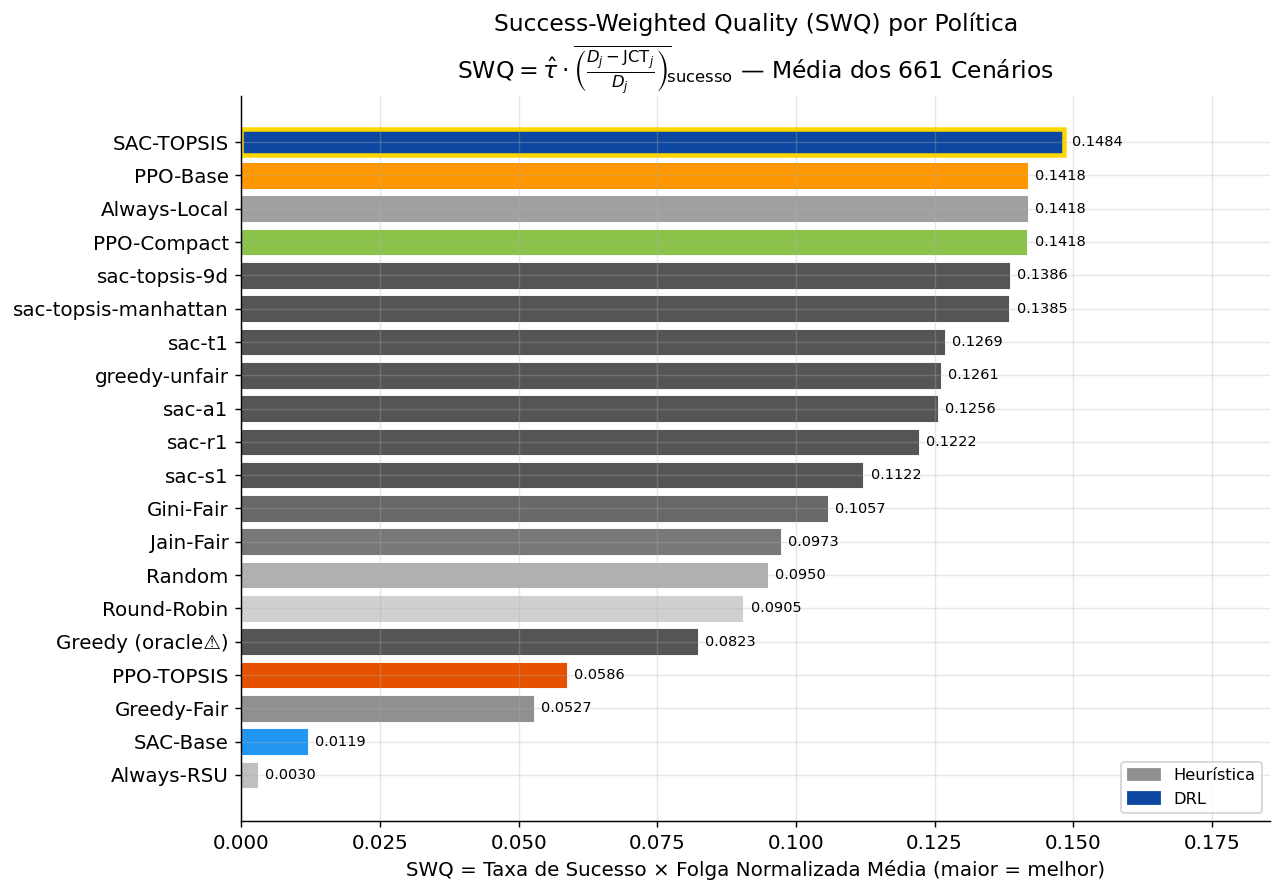
\includegraphics[width=\textwidth]{figuras/performance_09_swq.png}
\caption{SWQ médio por política sobre 661 cenários de teste ($\alpha=0{,}35$, $\beta=0{,}35$, $\gamma=0{,}30$). Barras em cinza representam heurísticas; barras escuras representam políticas \gls{DRL}. A borda dourada indica a melhor política. Maior é melhor.}
\label{fig:swq}
\end{figure}

\section{Por que o \gls{TOPSIS} agrega valor ao \gls{SAC} mas não ao \gls{PPO}?}
\label{sec:sac-topsis-sinergia}

Os resultados experimentais revelam uma assimetria marcante: o \gls{TOPSIS} eleva a taxa de \textit{deadline} do \gls{SAC} de $4{,}6\%$ (SAC-Base) para $45{,}3\%$ (SAC-TOPSIS), um ganho de $+40{,}7$ pontos percentuais, enquanto o \gls{PPO} com \gls{TOPSIS} regride. Para isolar a causa desta assimetria, foram realizados dois experimentos controlados. Primeiro, o PPO-TOPSIS original com estado 12D e ação ternária --- que permitia ao agente escolher entre rank$_1$, rank$_2$ e rank$_3$ --- obteve $18{,}4\%$, abaixo do PPO-Base ($42{,}4\%$). Segundo, o PPO-TOPSIS foi refatorado para utilizar \emph{exatamente} o mesmo estado 6D, ação binária $\{0\!=\!\text{LOCAL},\, 1\!=\!\text{rank}_1\}$ e função de recompensa do SAC-TOPSIS, diferindo apenas no algoritmo de otimização (\gls{PPO} vs.\ \gls{SAC}). O resultado deste experimento controlado foi igualmente $18{,}4\%$, com a política colapsando para $86\%$ de \textit{offload} via rank$_1$ --- o oposto do PPO-Compact ($100\%$ LOCAL), porém igualmente disfuncional. O PPO-TOPSIS-Compact, que usa o estado 6D mas foi treinado em cenários distintos, apenas iguala o PPO-Base. Em síntese: \textbf{o \gls{TOPSIS} é uma alavanca decisiva para o \gls{SAC} e um fator neutro ou prejudicial para o \gls{PPO}, independentemente do design do estado}. Esta seção analisa as causas estruturais desta assimetria.

\subsection{O problema do aprendizado redundante no PPO-TOPSIS}

O PPO-TOPSIS foi implementado com um estado de 12 dimensões --- três alternativas (LOCAL, \gls{RSU}, \gls{V2V}) ordenadas pelo escore \gls{TOPSIS}, cada uma descrita por quatro atributos normalizados (JCT estimado, energia, distância, \textit{link lifetime}) --- e um espaço de ação ternário $a_t \in \{0\!=\!\text{rank}_1,\, 1\!=\!\text{rank}_2,\, 2\!=\!\text{rank}_3\}$. Esse design cria um problema de \textbf{aprendizado redundante}: o \gls{TOPSIS} já determina deterministicamente que o candidato na posição 0 é o melhor segundo critérios multicritério rigorosos. O agente \gls{PPO}, portanto, é treinado por reforço para redescobrir, por tentativa e erro, o que o \gls{TOPSIS} já computou de forma ótima. A informação de valor genuíno que o agente deveria aprender --- se há benefício em descarregar para o melhor candidato dado o estado da fila e a urgência do \textit{deadline} --- está enterrada sob o sinal dominante de que rank$_1$ é sempre superior a rank$_2$ e rank$_3$ em custo multicritério.

O SAC-TOPSIS resolve este problema por projeto: delega a pergunta \emph{``para onde descarregar?''} inteiramente ao \gls{TOPSIS} e reserva ao agente apenas a pergunta \emph{``descarregar ou não?''} --- uma decisão genuinamente nova, que o \gls{TOPSIS} não responde, pois envolve a comparação entre o melhor candidato de \textit{offload} e a execução local ponderada pela urgência temporal, pelo congestionamento da fila e pela vantagem objetiva $\Delta_{\text{obj}}$ codificada no estado 6D.

\subsection{Colapso de política induzido pelo sinal TOPSIS}

O segundo mecanismo de falha do PPO-TOPSIS é o \textbf{colapso de política}. Com o estado 12D, a posição rank$_1$ exibe consistentemente JCT menor, energia menor e distância menor que rank$_2$ e rank$_3$. Isso gera um gradiente de política fortemente unidirecional desde as primeiras iterações: $P(a\!=\!0) \to 1$. O \gls{PPO} utiliza coeficiente de entropia $\alpha_{\text{ent}} = 0{,}01$, dez vezes menor que o do \gls{SAC} ($\alpha_{\text{ent}} = 0{,}10$ com ajuste automático via gradiente dual). Com entropia tão fraca, uma vez que a distribuição de política colapsa para $P(\text{rank}_1) \approx 1$, as trajetórias coletadas nas iterações seguintes são quase exclusivamente de escolhas rank$_1$, reforçando o colapso. O mecanismo de \textit{clipping} do \gls{PPO} ($\epsilon = 0{,}2$) não reverte esse estado: ele apenas impede mudanças \emph{grandes} por passo, mas não impede a deriva acumulada durante os 400 episódios de treinamento.

O \gls{SAC}, ao contrário, opera sobre um espaço de ação binário em que nenhuma das duas opções (LOCAL ou \textit{offload} para rank$_1$) domina o outro de forma incondicional: há cenários em que a fila do \gls{RSU} está saturada, ou o \gls{V2V} está distante, ou o \textit{deadline} é tão apertado que mesmo o melhor candidato de \textit{offload} não chega a tempo. Nesses casos, a resposta correta é LOCAL, e o sinal de recompensa deadline-aware --- com lacuna mínima de $1{,}5$ entre o melhor valor de falha e o pior valor de sucesso --- preserva um gradiente exploratório relevante. A alta temperatura entrópica do \gls{SAC} garante que ambas as ações recebam probabilidade não nula ao longo do treinamento, evitando o colapso.

\subsection{Assimetria de eficiência amostral com cenário único}

O protocolo de treinamento emprega \textbf{um único cenário} (\texttt{cenario\_v2x\_10tps\_w01}) durante os 400 episódios, com generalização \textit{zero-shot} para os 661 cenários de teste. Essa escolha é compatível com o \gls{SAC}, mas estruturalmente adversa ao \gls{PPO}.

O \gls{SAC} mantém um \textit{replay buffer} de 50.000 transições e realiza atualizações com \textit{minibatch} de 1024 amostras por passo. Com aproximadamente 100 tarefas por episódio, as 40.000 transições coletadas ao longo dos 400 episódios são amostradas em média $\approx\!40$ vezes cada durante o treinamento --- uma reciclagem intensiva que extrai máxima informação de um conjunto de dados limitado. Além disso, a mistura de experiências de diferentes pontos do treinamento (política mais aleatória nos primeiros episódios, mais refinada nos últimos) cria uma diversidade implícita que previne o sobreajuste ao único cenário de treino.

O \gls{PPO}, sendo \textit{on-policy}, descarta cada lote de trajetórias após as $k\!=\!8$ épocas de atualização. Com um único cenário, cada episódio gera essencialmente o mesmo padrão de chegada de tarefas, o mesmo volume de tarefas e as mesmas condições de canal. A política converge rapidamente para a estratégia que maximiza a recompensa nesse cenário específico --- que, com a salência do sinal \gls{TOPSIS}, é \emph{``sempre escolha rank$_1$''} --- e não tem como escapar desse ótimo local por falta de diversidade nos dados on-policy.

A evidência experimental confirma esta hipótese: o PPO-TOPSIS-Compact, que usa o estado 6D do SAC-TOPSIS (idêntico em conteúdo semântico) mas com algoritmo \gls{PPO}, atinge $42{,}4\%$ --- o mesmo que o PPO-Base, que usa o estado bruto 11D. O estado \gls{TOPSIS} mais informativo não agrega valor ao \gls{PPO} porque o gargalo não é a qualidade do estado, mas a ineficiência amostral do algoritmo on-policy com cenário único.

\subsection{Síntese: complementaridade estrutural SAC--TOPSIS}

A superioridade do SAC-TOPSIS não decorre de nenhum componente isolado, mas da \textbf{complementaridade estrutural} entre os dois módulos em três dimensões:

\begin{enumerate}
    \item \textbf{Divisão de responsabilidades}: O \gls{TOPSIS} resolve deterministicamente a pergunta \emph{``qual candidato de \textit{offload} é melhor?''}; o \gls{SAC} aprende a resposta à pergunta complementar \emph{``vale a pena descarregar para esse candidato?''}. As duas perguntas são independentes e igualmente necessárias; nenhum dos dois módulos, isoladamente, as responde ambas.

    \item \textbf{Off-policy + replay buffer}: O \gls{SAC} recicla cada transição $\approx\!40$ vezes no treinamento com um único cenário, alcançando uma eficiência amostral inacessível ao \gls{PPO} on-policy. Essa reciclagem é segura porque o \gls{SAC} aprende uma função de valor $Q(s,a)$ que é off-policy por construção --- ao contrário do \gls{PPO}, cujo gradiente de política requer dados coletados pela política corrente.

    \item \textbf{Regularização entrópica intensa}: O \gls{SAC} mantém $\alpha_{\text{ent}} = 0{,}10$ com ajuste automático, dez vezes superior ao coeficiente fixo do \gls{PPO}. Essa entropia elevada é precisamente o que impede o colapso de política frente ao sinal claro fornecido por $\Delta_{\text{obj}}$ no estado 6D --- mantendo a exploração ativa mesmo quando o \gls{TOPSIS} sugere fortemente que \textit{offload} é melhor.
\end{enumerate}

Em contraste, o PPO-TOPSIS sofre das três falhas simétricas: aprende uma pergunta que o \gls{TOPSIS} já responde (redundância), colapsa para uma estratégia degenerada com entropia insuficiente para resistir ao sinal \gls{TOPSIS} (colapso), e sobreajusta ao único cenário de treino sem o mecanismo de reciclagem do \textit{replay buffer} (ineficiência amostral). O experimento controlado confirma inequivocamente este diagnóstico: ao trocar \emph{apenas} o algoritmo --- mantendo estado 6D, ação binária e recompensa idênticos --- o SAC-TOPSIS atinge $45{,}3\%$ enquanto o PPO-TOPSIS obtém $18{,}4\%$, um déficit de $26{,}9$ pontos percentuais atribuível exclusivamente à natureza on-policy do \gls{PPO} e à sua baixa temperatura entrópica. O \gls{TOPSIS}, portanto, não é neutro quando mal integrado: \emph{amplifica} as fraquezas do algoritmo hospedeiro.

% ──────────────────────────────────────────────────────────────────────────────
\section{Avaliação Comparativa de Políticas}
\label{sec:ranking-completo}

As Tabelas~\ref{tab:ranking-completo} e~\ref{tab:ganho-topsis} resumem os resultados de 25 políticas avaliadas em 658 cenários de teste comuns, abrangendo algoritmos de aprendizado por reforço (com e sem \gls{TOPSIS}) e heurísticas de referência. As métricas reportadas são: taxa de \textit{deadline} (\%), SWQ ($= \hat{\tau}\cdot\overline{(D_j - \text{JCT}_j)/D_j}_{\text{sucesso}}$), JCT médio em segundos, energia média por tarefa em joules e o objetivo $J(\pi) = 0{,}60\cdot\hat{\tau} - 0{,}40\cdot\overline{(0{,}35\,\text{JCT} + 0{,}35\,E)/(D + 0{,}35\,E_{\max})}$ com $E_{\max} = 432{,}6\,\text{J}$ (percentil 99 global).

\begin{landscape}
\begin{table}[htbp]
\centering
\caption{Ranking completo das 25 políticas avaliadas em 658 cenários comuns (ordenado por SWQ decrescente). $\star$~=~usa \gls{TOPSIS}.}
\label{tab:ranking-completo}
\resizebox{\linewidth}{!}{%
\begin{tabular}{clrrrrrrrrr}
\toprule
\textbf{\#} & \textbf{Política} & \textbf{Cn} & \textbf{Taxa\%} & \textbf{SWQ} & \textbf{JCT (s)} & \textbf{E (J)} & \textbf{J($\pi$)} & \textbf{\%Loc} & \textbf{\%V2V} & \textbf{Categoria} \\
\midrule
 1 & \textbf{sac-topsis} $\star$       & 658 & \textbf{45,21} & \textbf{0,1484} &  6,547 & 25,828 & \textbf{0,2454} & 74,1 & 25,9 & RL+TOPSIS \\
 2 & ppo-topsis $\star$                & 658 & 42,66 & 0,1426 &  5,895 & 21,333 & 0,2344 & 98,7 &  1,3 & RL+TOPSIS \\
 3 & ppo-base                    & 658 & 42,32 & 0,1418 &  6,045 & 24,414 & 0,2295 & 100,0 &  0,0 & RL-Base \\
 4 & ppo-topsis-compact $\star$        & 658 & 42,32 & 0,1418 &  6,045 & 24,414 & 0,2295 & 100,0 &  0,0 & RL+TOPSIS \\
 5 & td3-base                    & 658 & 42,32 & 0,1418 &  6,045 & 24,414 & 0,2295 & 100,0 &  0,0 & RL-Base \\
 6 & a2c-topsis $\star$                & 658 & 42,32 & 0,1418 &  6,045 & 24,414 & 0,2295 & 100,0 &  0,0 & RL+TOPSIS \\
 7 & td3-topsis $\star$                & 658 & 43,91 & 0,1388 &  \textbf{3,703} & 22,995 & 0,2424 & 76,5 & 23,5 & RL+TOPSIS \\
 8 & sac-topsis-9d $\star$             & 658 & 42,82 & 0,1386 &  5,886 & \textbf{20,985} & 0,2348 & 94,7 &  5,3 & RL+TOPSIS \\
 9 & sac-topsis-manhattan $\star$      & 658 & 41,66 & 0,1385 & 11,831 & 23,656 & 0,2211 & 51,1 & 48,9 & RL+TOPSIS \\
10 & sac-t1 $\star$                    & 658 & 32,96 & 0,1270 & 11,487 & 26,126 & 0,1658 & 22,6 & 77,4 & RL+TOPSIS \\
11 & greedy-unfair               & 658 & 41,29 & 0,1262 &  5,613 &  7,396 & 0,2370 & 67,3 & 32,7 & Heurística \\
12 & sac-a1                      & 658 & 39,11 & 0,1256 & 13,722 & 21,118 & 0,2064 & 82,9 & 17,1 & RL-Base \\
13 & sac-r1                      & 658 & 38,26 & 0,1223 & 13,353 & 31,425 & 0,1914 & 58,8 & 41,2 & RL-Base \\
14 & sac-s1                      & 658 & 28,69 & 0,1122 & 39,298 & 20,305 & 0,1210 & 38,2 & 61,8 & RL-Base \\
15 & gini                        & 658 & 35,24 & 0,1057 &  3,456 & 39,395 & 0,1790 & 61,7 & 38,3 & Heurística \\
16 & dqn-topsis $\star$                & 658 & 25,90 & 0,0997 & 21,722 & 23,979 & 0,1161 & 20,0 & 80,0 & RL+TOPSIS \\
17 & jain                        & 658 & 32,54 & 0,0973 &  3,628 & 39,280 & 0,1627 & 58,6 & 41,4 & Heurística \\
18 & random                      & 658 & 30,02 & 0,0950 & 17,853 & 27,330 & 0,1427 & 40,7 & 59,3 & Heurística \\
19 & roundrobin                  & 658 & 28,50 & 0,0905 & 17,900 & 31,080 & 0,1315 & 34,9 & 65,1 & Heurística \\
20 & greedy                      & 658 & 29,03 & 0,0823 & 29,265 &  6,168 & 0,1429 & 42,5 & 57,5 & Heurística \\
21 & a2c-base                    & 658 & 21,74 & 0,0772 & 13,653 & 48,862 & 0,0785 & 20,3 & 79,7 & RL-Base \\
22 & dqn-base                    & 658 & 22,10 & 0,0686 & 13,599 & 44,445 & 0,0839 & 21,5 & 78,5 & RL-Base \\
23 & greedy-fair                 & 658 & 20,61 & 0,0528 & 40,754 &  \textbf{5,634} & 0,0823 & 27,9 & 72,1 & Heurística \\
24 & sac-base                    & 658 &  4,52 & 0,0119 & 57,075 & 24,230 & $-$0,042 &  5,1 & 94,9 & RL-Base \\
25 & rsu                         & 658 &  1,86 & 0,0030 & 144,191 & 4,843 & $-$0,123 &  1,2 & 98,8 & Heurística \\
\bottomrule
\end{tabular}%
}
\end{table}
\end{landscape}

A Tabela~\ref{tab:ganho-topsis} isola o efeito do \gls{TOPSIS} para cada família de algoritmos, comparando a versão base com a versão aumentada pelo ranqueamento multicritério.

\begin{table}[htbp]
\centering
\caption{Ganho do \gls{TOPSIS} por família de algoritmo (médias sobre 658 cenários comuns). $\Delta$Taxa e $\Delta$SWQ representam diferença absoluta; $\Delta$J($\pi$) é a diferença na função objetivo.}
\label{tab:ganho-topsis}
\small
\resizebox{\textwidth}{!}{%
\begin{tabular}{llrrrrrrr}
\toprule
\multirow{2}{*}{\textbf{Algoritmo}} & \multirow{2}{*}{\textbf{Versão}} & \multicolumn{2}{c}{\textbf{Taxa\%}} & \multicolumn{2}{c}{\textbf{SWQ}} & \multicolumn{2}{c}{\textbf{J($\pi$)}} & \multirow{2}{*}{\textbf{Destaques}} \\
\cmidrule(lr){3-4}\cmidrule(lr){5-6}\cmidrule(lr){7-8}
 & & Base & \gls{TOPSIS} & Base & \gls{TOPSIS} & Base & \gls{TOPSIS} & \\
\midrule
\multirow{2}{*}{SAC}
 & base   & 4,52  & ---    & 0,0119 & ---    & $-$0,042 & --- & colapso total (94,9\% \gls{V2V}) \\
 & topsis & ---   & \textbf{45,21} & ---    & \textbf{0,1484} & --- & \textbf{0,2454} & \textbf{$+$40,7 pp / $+$1147\% SWQ} \\
\midrule
\multirow{2}{*}{PPO}
 & base   & 42,32 & ---    & 0,1418 & ---    & 0,2295 & --- & 100\% local \\
 & topsis & ---   & 42,66  & ---    & 0,1426 & --- & 0,2344 & $+$0,3 pp / $+$0,6\% SWQ \\
\midrule
\multirow{2}{*}{TD3}
 & base   & 42,32 & ---    & 0,1418 & ---    & 0,2295 & --- & 100\% local \\
 & topsis & ---   & 43,91  & ---    & 0,1388 & --- & 0,2424 & $+$1,6 pp taxa; JCT $-44{,}5\%$ \\
\midrule
\multirow{2}{*}{DQN}
 & base   & 22,10 & ---    & 0,0686 & ---    & 0,0839 & --- & 78,5\% \gls{V2V} sem critério \\
 & topsis & ---   & 25,90  & ---    & 0,0997 & --- & 0,1161 & $+$3,8 pp / $+$45\% SWQ \\
\midrule
\multirow{2}{*}{A2C}
 & base   & 21,74 & ---    & 0,0772 & ---    & 0,0785 & --- & 79,7\% \gls{V2V}, energia alta \\
 & topsis & ---   & 42,32  & ---    & 0,1418 & --- & 0,2295 & \textbf{$+$20,6 pp / $+$84\% SWQ} \\
\bottomrule
\end{tabular}%
}
\end{table}

	\chapter{Conclusões}
\label{chap:conclusoes}

Este capítulo sintetiza as contribuições alcançadas nesta etapa de qualificação, interpreta os resultados experimentais obtidos, aponta as limitações identificadas e delineia os trabalhos futuros necessários para a consolidação da tese. O objetivo principal da proposta é a integração entre o ranqueamento multicritério por \gls{TOPSIS} e o \gls{DRL} baseado no algoritmo \gls{SAC}, motivada pela necessidade de resolver o problema de descarregamento de tarefas em redes \gls{VEC} de forma adaptativa, escalável e capaz de atender aos requisitos de prazo sem necessidade de retreinamento diante de variações na topologia veicular.

\section{Contribuições Alcançadas}
\label{sec:contribuicoes-alcancadas}

A contribuição central deste trabalho consiste na proposição e validação de uma arquitetura de decisão que divide responsabilidades de forma entre dois módulos complementares. O módulo \gls{TOPSIS} avalia, a cada instante de decisão, o conjunto de candidatos ao descarregamento segundo o tempo de conclusão estimado (\gls{JCT}), a energia total e a distância ao nó de computação, condensando essas informações em um vetor de estado compacto de seis dimensões. Esse vetor é invariante ao número de candidatos presentes, resolvendo o problema do número de entradas variável que afeta a maioria das abordagens de \gls{DRL} puro no domínio veicular~\cite{uddin2025, tang2024}. A partir dessa representação, o módulo \gls{SAC} aprende uma política de decisão binária beneficiando-se da regularização por entropia máxima para manter a exploração ativa em ambientes não-estacionários~\cite{haarnoja2018sac}.

A representação do espaço de estado compacto 6D é outra contribuição direta deste trabalho. Cada dimensão dela carrega significado semântico relativo para a decisão. Em conjunto, essas seis dimensões fornecem ao agente uma visão comprimida e suficientemente rica para avaliar, a cada decisão, a vantagem relativa do descarregamento frente à execução local.

Igualmente relevante é a engenharia da função de recompensa \textit{deadline-aware} (Equação~\ref{eq:reward}). Ao introduzir intencionalmente uma lacuna entre o pior cenário de sucesso e o melhor cenário de falha, a formulação estabelece que cumprir o prazo é sempre preferível a qualquer execução tardia, independentemente do ganho energético associado. Essa descontinuidade, que demarcaria uma fronteira de aprendizado problemática para algoritmos baseados em valor e justifica estruturalmente a adoção do \gls{SAC}~\cite{ng1999policy, haarnoja2018sac}.

% Do ponto de vista da infraestrutura experimental, este trabalho desenvolveu um simulador de eventos discretos (\gls{DES}) implementado em C++20 com co-rotinas, utilizando a biblioteca \texttt{simcpp20}~\cite{simcpp20}. O simulador integra mobilidade veicular gerada pelo SUMO~\cite{lopez2018microscopic}, carga de trabalho derivada do \textit{trace} real de demandas computacionais do Alibaba~\cite{cheng2018characterizing} e modelos de canal compatíveis com as diretrizes do \gls{3GPP} TR~38.901 para enlaces \gls{V2I} e TR~37.885 para enlaces \gls{V2V}~\cite{3gpp38901, 3gpp_tr37885}. Essa base experimental, composta por 658 cenários de teste com taxas de chegada variando entre 10 e 45 tarefas por segundo, garante que os resultados reportados sejam representativos de uma ampla gama de regimes de tráfego, incluindo condições de carga leve, moderada e severa.

Por fim, a proposição da métrica \gls{SWQ} (Equação~\ref{eq:swq}) ajuda a medir a qualidade da política como o produto da taxa de sucesso pelo valor esperado da folga normalizada das tarefas concluídas no prazo, a métrica supera as limitações da taxa de sucesso simples, em que as tarefas bem-sucedidas e as falhas se mesclam sem discriminação. O \gls{SWQ} contribui de maneira mais adequada na comparação de políticas em ambientes com prazos heterogêneos e alta variância de carga.

\section{Síntese dos Resultados Experimentais Preliminares}
\label{sec:sintese-resultados}

A avaliação comparativa envolvendo 21 políticas sobre 658 cenários de teste comuns confirma a superioridade da arquitetura proposta. O \gls{SAC}-FTOPSIS alcançou a maior taxa de sucesso (45,21\%) e o maior \gls{SWQ} (0,1484) entre todos os métodos avaliados, incluindo heurísticas gulosas com acesso privilegiado ao estado real das filas (\textit{Greedy-Unfair}, \gls{SWQ} = 0,1262). O \gls{JCT} médio da proposta (6,547~s) é 8,6 vezes inferior ao do \gls{SAC}-Base (57,075~s), indicando que a combinação entre compressão de estado via \gls{TOPSIS}, recompensa sensível ao prazo e ação binária produz não apenas mais tarefas concluídas no prazo, mas também latências substancialmente menores.

O estudo de ablação controlado com cinco variantes (Base, A1, S1, R1 e T1) decompose causalmente o ganho total de $+40{,}69$ pontos percentuais (\textit{pp}) sobre o \gls{SAC}-Base, conforme sintetizado na Equação~\ref{eq:decomposicao}. A maior parcela do ganho provém da compressão de estado de 11D para 6D (Base $\to$ S1: $+24{,}17$~pp), evidenciando que a redução da dimensionalidade e a estruturação semântica da entrada são os fatores mais determinantes para a convergência do agente. A adoção do \gls{TOPSIS} como responsável pela decisão de destino (T1 $\to$ \gls{SAC}-FTOPSIS: $+12{,}25$~pp) é o segundo maior contribuinte, indicando que eliminar a ambiguidade \gls{VEC}/\gls{V2V} do espaço de ação do agente aumenta significativamente a eficácia do aprendizado. A incorporação do escore \gls{TOPSIS} como \textit{feature} de estado combinada com a recompensa \textit{deadline-aware} (S1 $\to$ T1: $+4{,}27$~pp) apresenta contribuição marginal mais modesta.

% A hierarquia de contribuição dos componentes, sintetizada na expressão
% \[
%     \Delta_{\text{estado}} > \Delta_{\text{TOPSIS-decisão}} > \Delta_{\text{reward+feature}} \gg \Delta_{\text{ação-binária-estática}},
% \]
% indica que a arquitetura \gls{SAC}-FTOPSIS é fundamentalmente uma solução de \textit{divisão de responsabilidades}: o \gls{TOPSIS} resolve deterministicamente a pergunta \textit{``para qual candidato descarregar?''}, enquanto o \gls{SAC} aprende a resposta à pergunta complementar \textit{``vale a pena descarregar para esse candidato dado o estado atual das filas, o prazo e a vantagem relativa?''} --- uma pergunta que o \gls{TOPSIS} isoladamente não é capaz de responder.

% Adicionalmente, os resultados revelam que a estratégia ótima de descarregamento, em termos de maximização do \gls{SWQ}, passa pela priorização do processamento local: as melhores políticas do \textit{ranking} exibem taxas de execução local elevadas (\%Loc próximo a 100\% no \gls{PPO} e \gls{TD3}, e 74,1\% no \gls{SAC}-FTOPSIS), indicando que o descarregamento remoto só agrega valor quando a janela temporal disponível compensa os atrasos de transmissão e de fila. Essa constatação corrobora a premissa do modelo de recompensa adotado, em que a penalidade por violação de prazo é estruturalmente dominante sobre qualquer ganho de eficiência energética.

\section{Limitações e Questões em Aberto}
\label{sec:limitacoes}

Embora os resultados sejam promissores, uma análise rigorosa impõe o reconhecimento das limitações presentes nesta fase do trabalho. A mais relevante delas reside no protocolo de treinamento: o agente é treinado em um único cenário de 10~tps com 100 tarefas e avaliado em modo \textit{zero-shot} sobre 658 cenários com taxas de chegada distintas (até 45~tps). A generalização observada demonstra que a representação 6D do \gls{TOPSIS} é suficientemente compacta para interpolação entre regimes de carga, porém não garante robustez máxima em cenários extremos ainda não representados durante o treinamento. A extensão do protocolo de treinamento para múltiplos cenários e regimes de carga é, portanto, uma necessidade para a validação definitiva.

% O modelo atual assume plena capacidade de estimar o \gls{JCT} remoto no instante da decisão, o que pressupõe acesso ao estado real das filas dos servidores candidatos. Em redes veiculares reais, essa informação chega com atraso de telemetria e pode estar desatualizada devido à alta mobilidade dos nós~\cite{liu2025, abbas2025}. A incorporação explícita de incerteza de medição --- prevista na etapa de evolução para o \textit{Fuzzy}-\gls{TOPSIS} --- é um passo indispensável para aproximar o modelo das condições operacionais reais.

% A formulação atual restringe o descarregamento ao modo binário (\textit{full offloading}): a tarefa é executada integralmente no nó local ou integralmente no candidato de maior pontuação pelo \gls{TOPSIS}. Cenários com tarefas de alta demanda computacional poderiam se beneficiar de mecanismos de particionamento (\textit{partial offloading}), em que uma fração da tarefa é enviada ao servidor enquanto o restante é processado localmente em paralelo. Essa extensão amplia o espaço de ação para um domínio contínuo, o que demanda ajustes tanto na formulação do \gls{MDP} quanto na arquitetura do agente.

Por fim, o simulador atual opera sob a premissa de canal de comunicação simplificado, sem modelagem mais detalhada de desvanecimento rápido, interferência entre enlaces ou bloqueio de sinal. A integração com o simulador de rede ns-3 viabilizará a avaliação sob condições de propagação mais próximas do padrão \gls{3GPP} TR~38.901, incluindo os efeitos de mobilidade sobre a qualidade do enlace \gls{V2I} e \gls{V2V}.

\section{Proposta Final}
\label{sec:proposta-final}

A evolução planejada para a tese consiste na substituição do módulo \gls{TOPSIS} pelo \textit{Fuzzy}-\gls{TOPSIS}~\cite{chen2000}. A incorporação de \glspl{TFN} aos critérios de avaliação dos candidatos permitirá que a incerteza e a imprecisão das medições do ambiente veicular sejam formalmente representadas no processo de ranqueamento, em vez de serem ignoradas ou absorvidas imperfeitamente pela rede neural. Essa mudança não altera a interface entre os dois módulos (o vetor 6D continua sendo o contrato entre o \gls{TOPSIS} e o \gls{SAC}), mas enriquece semanticamente o conteúdo do estado entregue ao agente.

Por fim, planeja-se avaliar a proposta com o par ns-3/SUMO. Essa integração viabilizará a avaliação do \gls{SAC}-FTOPSIS em um ambiente de simulação de rede de eventos discretos completo, com modelagem realista das camadas \gls{PHY} e \gls{MAC} do \gls{5G} \gls{NR} e dos canais \gls{V2X} \textit{Sidelink}, superando a simplificação do canal perfeito adotada nesta fase.

% Por fim, planeja-se a avaliação de mecanismos de aprendizado contínuo (\textit{online learning}) que permitam ao agente atualizar incrementalmente sua política durante a operação em produção, sem a necessidade de retreinamento completo. Essa capacidade é fundamental para lidar com mudanças de distribuição de carga (\textit{distribution shifts}) causadas por eventos imprevistos sem degradação de desempenho.

% Por fim, a extensão para cenários multiagente, em que múltiplos veículos operam simultaneamente sobre uma infraestrutura de borda compartilhada, introduz o problema de não-estacionariedade competitiva: as decisões concorrentes de agentes independentes alteram dinamicamente o estado das filas, potencialmente invalidando as estimativas locais de \gls{JCT}. A modelagem dessa interação --- seja por \gls{MARL} ou por mecanismos de coordenação explícita --- representa uma fronteira científica relevante para a fase final da tese.

\section{Considerações Finais}
\label{sec:consideracoes-finais}

Este documento de qualificação demonstra a viabilidade científica e experimental da arquitetura \gls{SAC}-FTOPSIS para o descarregamento adaptativo de tarefas em redes \gls{VEC}. O conjunto de contribuições alcançadas estabelece uma base teórica e metodológica sólida sobre a qual a tese final será construída.

A proposta responde diretamente às lacunas identificadas na revisão de literatura, conforme sintetizado na Tabela~\ref{tab:lacunas-atendidas}. Em particular, a arquitetura resolve a ausência de representações de estado escaláveis ao número variável de candidatos~\cite{miriyala2026, uddin2025}, a predominância de modelagens com observabilidade perfeita~\cite{liu2025} e a falta de políticas avaliadas sob diferentes regimes de carga~\cite{Moghaddasi2023}. Os resultados obtidos com o \gls{SAC}-FTOPSIS constituem evidência empírica de que a divisão de responsabilidades entre ranqueamento multicritério e aprendizado por reforço profundo é uma estratégia eficaz para o domínio veicular.

\begin{table}[ht!]
    \centering
    \Caption{\label{tab:lacunas-atendidas} Lacunas de pesquisa atendidas pela proposta (baseado em~\citeonline{miriyala2026}).}
    \UECEtab{}{% 
        \begin{tabular}{|c|p{4.5cm}|p{6.5cm}|c|}
            \hline
            \textbf{\#} & \textbf{Lacuna Identificada} & \textbf{Resposta da Proposta} & \textbf{Status} \\ \hline
            1 & \textit{Flat vectors} ignoram topologia variável ($N$ nós) & \gls{TOPSIS} comprime $N$ candidatos em vetor 6D fixo (invariante à escala). & Sim \\ \hline
            2 & Políticas estáticas colapsam sob alta mobilidade & \gls{SAC} com entropia máxima e \textit{replay buffer} para adaptação contínua. & Sim \\ \hline
            3 & Vulnerabilidade a ruído nas observações de estado & Estado 6D normalizado via \textit{Fuzzy}-\gls{TOPSIS} atenua sensibilidade a \textit{outliers}. & Parcial \\ \hline
            4 & Modelos leves para borda extrema (\textless 50 MB) & MLP $6{\to}64{\to}64{\to}2$ ($\approx$ 8 KB); inferência em microssegundos. & Sim \\ \hline
            5 & \textit{Continual learning} sem \textit{catastrophic forgetting} & Treinamento \textit{off-policy} com memória de experiência para atualização incremental. & Sim \\ \hline
        \end{tabular} 
    }{% 
        \Fonte{Adaptado de~\citeonline{miriyala2026}.}
    }
\end{table}

Os próximos passos, detalhados no cronograma da Tabela~\ref{tab:cronograma}, contemplam a integração com o \textit{Fuzzy}-\gls{TOPSIS}, a co-simulação com ns-3/SUMO, o refinamento do agente e a análise comparativa estendida. Espera-se que a tese final contribua de forma original e significativa para o campo de gerenciamento de recursos em sistemas de transporte inteligentes de próxima geração, com resultados a serem submetidos a periódicos de alto impacto, como o IEEE Transactions on Intelligent Transportation Systems e o IEEE Transactions on Vehicular Technology.

\section{Cronograma de Pesquisa}
\label{sec:cronograma}

A Tabela~\ref{tab:cronograma} apresenta as atividades de pesquisa e o cronograma de conclusão, detalhado por semestre (S1, S2) e trimestre (Q1).

\begin{table}[ht!]
    \centering
    \Caption{\label{tab:cronograma} Atividades de pesquisa e cronograma de conclusão (2026--2028).}
    \UECEtab{}{% 
        \begin{tabular}{|l|c|c|c|c|c|} 
            \hline
            \textbf{Atividade / Ano} & \multicolumn{2}{c|}{\textbf{2026}} & \multicolumn{2}{c|}{\textbf{2027}} & \textbf{2028} \\ \cline{2-6}
            & S1 & S2 & S1 & S2 & Q1 \\ \hline
            1. Exame de Qualificação            & X &   &   &   &   \\ \hline
            2. Integração com Simulador (NS-3/SUMO) & X & X &   &   &   \\ \hline
            3. Refinamento de Algoritmos        & X & X & X &   &   \\ \hline
            4. Avaliação de Desempenho e Coleta de Dados &   & X & X &   &   \\ \hline
            5. Análise dos Resultados           &   &   & X & X &   \\ \hline
            6. Escrita da Tese Final            &   &   &   & X & X \\ \hline
            7. Defesa Final                     &   &   &   &   & X \\ \hline
        \end{tabular} 
    }{% 
        \Fonte{Elaborado pelo autor. S1: 1\textordmasculine{} semestre (jan.--jun.); S2: 2\textordmasculine{} semestre (jul.--dez.); Q1: 1\textordmasculine{} trimestre de 2028 (jan.--mar.).}
    }
\end{table}
\section{Plano de Publicação}
\label{sec:plano-publicacao}

A disseminação das descobertas focará em periódicos e conferências especializadas em redes veiculares, computação de borda e sistemas inteligentes. Os locais planejados priorizados para submissão incluem:

\begin{itemize}
    \item \textbf{Periódicos de Alto Impacto:}
    \begin{itemize}
        \item IEEE Transactions on Intelligent Transportation Systems (T-\gls{ITS});
        \item IEEE Transactions on Vehicular Technology (TVT);
        \item IEEE Transactions on Intelligent Vehicles (TIV);
        \item IEEE Transactions on Mobile Computing (TMC);
        \item IEEE Internet of Things Journal.
    \end{itemize}
    \item \textbf{Conferências Relevantes:}
    \begin{itemize}
        \item IEEE Vehicular Technology Conference (VTC);
        \item IEEE Global Communications Conference (GLOBECOM);
        \item IEEE International Conference on Communications (ICC).
    \end{itemize}
\end{itemize}

	\chapter{Cronograma de Pesquisa e Plano de Publicação}
\label{chap:cronograma-pesquisa}

Este capítulo detalha o roteiro para a conclusão da pesquisa de doutorado e a estratégia para a disseminação dos resultados através de publicações de alto impacto, considerando o prazo final em março de 2027.

\section{Cronograma de Pesquisa}
\label{sec:cronograma}

As atividades de pesquisa restantes estão estruturadas para garantir a conclusão do modelo Fuzzy-DRL e a validação experimental. A Tabela~\ref{tab:cronograma} apresenta o cronograma para o período de 2026 a 2027, culminando na defesa da tese.

\begin{table}[ht!]
    \centering
    \Caption{\label{tab:cronograma} Atividades de pesquisa e cronograma de conclusão (2026--2027).}
    \UECEtab{}{
        \begin{tabular}{|l|c|c|c|}
            \hline
            \textbf{Atividade / Ano} & \multicolumn{2}{c|}{\textbf{2026}} & \textbf{2027} \\ \cline{2-4}
                                     & \textbf{S1} & \textbf{S2} & \textbf{Q1} \\ \hline
            1. Exame de Qualificação     & X &   &   \\ \hline
            2. Integração com Simulador (NS-3/SUMO) & X & X &   \\ \hline
            3. Refinamento de Algoritmos & X & X &   \\ \hline
            4. Avaliação de Desempenho e Coleta de Dados &   & X &   \\ \hline
            5. Análise dos Resultados    &   & X & X \\ \hline
            6. Escrita da Tese Final     &   & X & X \\ \hline
            7. Defesa Final              &   &   & X \\ \hline
        \end{tabular}
    }{
        \Fonte{Elaborado pelo autor.}
    }
\end{table}

\section{Plano de Publicação}
\label{sec:plano-publicacao}

A disseminação das descobertas focará em periódicos e conferências especializadas em redes veiculares, computação de borda e sistemas inteligentes. Os locais planejados priorizados para submissão incluem:

\begin{itemize}
    \item \textbf{Periódicos de Alto Impacto:}
    \begin{itemize}
        \item IEEE Transactions on Intelligent Transportation Systems (T-ITS);
        \item IEEE Transactions on Vehicular Technology (TVT);
        \item IEEE Internet of Things Journal.
    \end{itemize}
    \item \textbf{Conferências Relevantes:}
    \begin{itemize}
        \item IEEE Vehicular Technology Conference (VTC);
        \item IEEE Global Communications Conference (GLOBECOM);
        \item IEEE International Conference on Communications (ICC).
    \end{itemize}
\end{itemize}

	% \chapter{Metodologia}
\label{chap:metodologia}

A metodologia deste trabalho é fundamentada na simulação, utilizando o simulador de redes NS-3, estendido com os módulos 5G-LENA e C-V2X para modelar com fidelidade o ambiente veicular 5G.

\section{Modelagem do Sistema e Formulação do Problema}
\label{sec:modelagem_sistema}

1. Entidades (unidade processadora, tarefa)
    1.1 Unidade Processadora (OBU e VEC)
        1.1.1 Fila de Processamento (tamanho maximo diferente durante a criaçao da unidade processadora)
        1.1.2 Fila de Transmissão (tamanho maximo diferente durante a criaçao da unidade processadora)
        1.1.3 Frequencia do Clock (GHZ)
            1.1.3.1 Modulo para criar perfil heterogeneo de CPU (maquinas lentas, medias, rapidas)
        1.1.4 Capacidade de Energia (Joules)
            1.1.4.1 Modulo para criar perfil heterogeneo de bateria
        1.1.5 Coeficiente de Eficiência Energética
            1.1.5.1 Modulo para criar perfil heterogeneo de consumo energetico
        1.1.6 Modelagem de Ambientes Não-Estacionários
            1.1.6.1 Drift nos Atributos da Unidade Processadora durante a simulação
    1.2 Tarefa
        1.2.1 Tamanho dos Dados de Entrada (tamanho maximo e minimo dependente do perfil de aplicação - bytes)
        1.2.2 Tamanho dos Dados de Saída (tamanho maximo e minimo dependente do perfil de aplicação - bytes)
        1.2.3 Atraso Máximo Tolerável (tamanho maximo e minimo dependente do perfil de aplicação - milisegundos)
        1.2.4 Densidade de Carga Computacional (tamanho maximo e minimo dependente do perfil de aplicação - ciclos de CPU por byte)
        1.2.5 Densidade de Carga Energética (tamanho maximo e minimo dependente do perfil de aplicação - joules por ciclo de CPU)
    1.3 Considerações sobre Geração de Tarefas
        1.3.1 Distribuição Estatística dos Atributos da Tarefa para diferentes perfis de aplicação
            1.3.1.1 Muitos dados e pouca computação
            1.3.1.2 Poucos dados e muitas computação
            1.3.1.3 Muitos dados e muita computação
            1.3.1.4 Poucos dados e pouca computação
            1.3.1.5 Media carga de dados e computação
        1.3.2 Modelagem de Ambientes Não-Estacionários
            1.3.2.1 Drift nos Atributos da Tarefa durante geração
    1.3 Considerações sobre Simulador de Eventos Discretos
        1.3.1 Adicionar na fila de processamento, remover da fila de processamento
        1.3.2 Adicionar na fila de transmissão, remover da fila de transmissão
        1.3.3 Iniciar processamento, finalizar processamento
        1.3.4 Iniciar transmissão, finalizar transmissão
    1.4 Incertezas na Modelagem
        1.4.1 Incerteza no tempo de processamento
        1.4.2 Incerteza no tempo de transmissão
        1.4.3 Incerteza no consumo energético
    1.4 Protocolo de descarregamento, na camada de aplicação
        1.4.1 Pedido de descarregamento
        1.4.2 Resposta ao Pedido (Aceite/Rejeição)
            1.4.2.1 Rejeição por fila cheia
            1.4.2.2 Rejeição por energia insuficiente
            1.4.2.3 Rejeição por não cumprimento do deadline
        1.4.3 Envio dos Dados da Tarefa
        1.4.4 Retorno do Resultado
        1.4.5 Confirmação de Recebimento do Resultado
        1.4.6 Timeouts e Retransmissões
        1.4.7 Medição de Métricas de Desempenho (latência, consumo energético, taxa de falhas, tamanho média das filas)
        1.4.8 Considerações sobre Simulador de Eventos Discretos
            1.4.8.1 Enviar pedido de descarregamento
            1.4.8.2 Aguardar resposta
    1.5 Protocolo de Descoberta de Vizinhança, na camada de aplicação
        1.5.1 Emissão de Beacons Periódicos (via 5G NR e V2X Sidelink)
            1.5.1.1 Conteúdo do Beacon (Device Specs, Estado Atual, velocidade, posição GPS, é VEC?, é OBU?, etc)
        1.5.2 Tabela de Vizinhos (Neighbor Table)
            1.5.2.1 Cálculo do Tempo de Vida Estimado do Enlace
            1.5.2.3 Atualização Periódica da Tabela de Vizinhos
            1.5.2.4 SNR, RSSI, CQI dos Vizinhos
2. Canal de comunicação
    2.1 Modelo de Canal 5G NR
        2.1.1 Taxa de Transmissão (Shannon-Hartley)
        2.1.2 Modelagem de Interferência
        2.1.3 Mobilidade Veicular e Variação do Canal
    2.2 Modelo de Canal V2X Sidelink (PC5)
        2.2.1 Taxa de Transmissão (Shannon-Hartley)
        2.2.2 Modelagem de Interferência
        2.2.3 Mobilidade Veicular e Variação do Canal
    2.3 Modelagem de Ambientes Não-Estacionários
        2.3.1 Drift nos Atributos do Canal durante a simulação
3. Descarregamento de tarefas
    3.1 Modos de Execução
        3.1.1 Processamento Local
        3.1.2 Descarregamento V2I (para RSU via 5G NR)
        3.1.3 Descarregamento V2V (para veículo vizinho via Sidelink)
    3.2
4. Coleta de métricas de desempenho do descarregamento de tarefas
    4.1 Métricas Globais
        4.1.1 Atraso Total do Sistema
        4.1.2 Consumo Energético Total do Sistema
        4.1.3 Índice de Justiça de Jain
        4.1.4 Taxa de Sucesso no descarregamento
        4.1.5 Total de Tarefas Processadas Localmente
        4.1.6 Total de Tarefas descarregadas via V2I
        4.1.7 Total de Tarefas descarregadas via V2V
    4.2 Métricas por Política de descarregamento
        4.2.1 Atraso Médio por Política
        4.2.2 Consumo Energético Médio por Política
        4.2.3 Taxa de Sucesso no descarregamento por Política
        4.3.4 Tamanho Médio das Filas por Política
        4.3.5 Índice de justiça de Jain por Política
    4.3 Análise de Sensibilidade
        4.3.1 Impacto dos Pesos na Função Objetivo
        4.3.2 Trade-off entre Latência, Consumo Energético e Justiça
    4.4 Função Objetivo Global
        4.4.1 Minimização do Atraso Total considerando incerteza
        4.4.2 Minimização do Consumo Energético Total considerando incerteza
        4.4.3 Maximização do Índice de Justiça de Jain
5. Integração com o SUMO
    5.1 Geração de Cenários Veiculares Realistas
        5.1.1 Cenário urbano com tráfego intenso, trafego moderado, tráfego leve
    5.2 Execução da simulação utilizando o SUMO para mobilidade veicular
9. Políticas de Decisão de descarregamento
    6.1 Políticas Heurísticas
        6.1.1 Processamento Local
        6.1.2 Descarregamento aleatório
        6.1.3 Descarregamento ganancioso
            6.1.3.1 Baseado na distancia ao VEC
            6.1.3.2 Baseado na qualidade do canal
            6.1.3.3 Baseado na latência
            6.1.3.4 Baseado no consumo energético
            6.1.3.5 Baseado na frequencia do clock do VEC
            6.1.3.6 Baseado no tempo de vida do enlaces
            6.1.3.7 Baseado na função objetivo
6. Criação de testes unitários para validação dos módulos desenvolvidos
    6.1 Testes para o módulo de geração de tarefas
    6.2 Testes para o módulo de modelagem do canal
    6.3 Testes para o módulo de descarregamento
    6.4 Testes para o protocolo de descoberta de vizinhança
    6.5 Testes para coleta de métricas de desempenho do descarregamento de tarefas
7. Usar docker para facilitar a reprodução dos experimentos
8. Usar script em bash e python para automatizar a execução dos experimentos e análise dos resultados
9. Criar logs para facilitar o rastreamento da execuçao do descarregamento (fim a fim)
10. Documentar o código desenvolvido utilizando Doxygen
11. Tratar exceções e erros durante a simulação para garantir robustez do sistema
    11.1 Não confiar 100 porcento nas entradas das funções, tratar todas as exceções possíveis



% Para validar a proposta de offloading em um cenário veicular heterogêneo operando sob cobertura 5G NR e comunicação V2X Sidelink, é fundamental estabelecer formalmente as entidades, as restrições físicas e os objetivos de otimização. Esta seção descreve o modelo matemático que fundamenta a arquitetura proposta.

% \subsection{Entidades e Heterogeneidade}

% Considere um cenário de rede veicular composto por um conjunto de veículos $\mathcal{V} = \{1, 2, \dots, V\}$ e um conjunto de RSUs (\textit{Road Side Units}) equipadas com servidores MEC, denotado por $\mathcal{R} = \{1, 2, \dots, R\}$.

% Cada veículo $i \in \mathcal{V}$ possui uma tarefa computacional atômica gerada no instante $t$, definida pela tupla $k_i = (D_i, C_i, T_i^{max})$, onde:
% \begin{itemize}
%     \item $D_i$: Tamanho dos dados de entrada da tarefa (em bits);
%     \item $C_i$: Custo computacional total (em ciclos de CPU);
%     \item $T_i^{max}$: Atraso máximo tolerado pela aplicação (latência crítica).
% \end{itemize}

% A heterogeneidade das OBUs (\textit{On-Board Units}) é modelada explicitamente através de parâmetros locais distintos para cada veículo $i$:
% \begin{equation}
%     \text{OBU}_i = \{ f_i^{loc}, P_i^{loc}, B_i^{rem} \}
% \end{equation}
% \noindent onde $f_i^{loc}$ é a frequência de clock da CPU local (ciclos/s), $P_i^{loc}$ é a potência de consumo computacional e $B_i^{rem}$ é a energia residual da bateria.

% \subsection{Modelos de Computação e Comunicação}

% O sistema permite três modos de execução: processamento local, offloading V2I (para RSU via 5G) e offloading V2V (para veículo vizinho via Sidelink).

% \subsubsection{Modelo de Computação Local}
% Caso o veículo decida processar a tarefa internamente, o tempo de execução $T_{i}^{loc}$ e o consumo energético $E_{i}^{loc}$ são dados por:
% \begin{equation}
%     T_{i}^{loc} = \frac{C_i}{f_i^{loc}}, \quad E_{i}^{loc} = \kappa (f_i^{loc})^2 C_i
% \end{equation}
% \noindent onde $\kappa$ é o coeficiente de eficiência energética dependente da arquitetura do chip.

% \subsubsection{Modelo de Comunicação (5G NR e Sidelink)}
% A taxa de transmissão $R_{i,j}$ entre o veículo $i$ e um nó de destino $j$ (seja $j \in \mathcal{R}$ ou $j \in \mathcal{V}$) é modelada pela lei de Shannon-Hartley para canais com ruído gaussiano:
% \begin{equation}
%     R_{i,j} = B \log_2 \left( 1 + \frac{P_i^{tx} |h_{i,j}|^2}{N_0 + I_{i,j}} \right)
% \end{equation}
% \noindent onde $B$ é a largura de banda do canal, $P_i^{tx}$ é a potência de transmissão, $h_{i,j}$ representa o ganho do canal (incluindo \textit{path loss} e desvanecimento) e $N_0$ é a densidade espectral de ruído. O termo $I_{i,j}$ representa a interferência, que é particularmente crítica nas comunicações V2V via Sidelink (PC5) devido ao reuso de recursos espaciais.

% \subsubsection{Modelo de Offloading}
% Se a tarefa é transferida para um nó remoto $j$, o tempo total $T_{i,j}^{off}$ compreende o tempo de transmissão e o processamento remoto:
% \begin{equation}
%     T_{i,j}^{off} = \frac{D_i}{R_{i,j}} + \frac{C_i}{f_j^{rem}}
% \end{equation}
% O consumo energético do veículo $i$ durante o offloading considera a energia de transmissão de rádio:
% \begin{equation}
%     E_{i,j}^{off} = P_i^{tx} \left( \frac{D_i}{R_{i,j}} \right) + E_{tail}
% \end{equation}

% \subsection{Formalização dos Objetivos e Otimização}

% O problema é modelado como uma otimização multi-objetivo visando minimizar o atraso e o consumo energético, enquanto maximiza a justiça (\textit{fairness}) entre os usuários. Seja $x_{i,j}$ uma variável binária de decisão, onde $x_{i,j}=1$ se o veículo $i$ processa no nó $j$ (sendo $j=0$ o processamento local).

% \subsubsection{Métricas Globais}
% O atraso total ($T_{sys}$) e a energia total ($E_{sys}$) do sistema são definidos como:
% \begin{equation}
%     T_{sys} = \sum_{i \in \mathcal{V}} \sum_{j \in \{0\} \cup \mathcal{V} \cup \mathcal{R}} x_{i,j} T_{i,j}
% \end{equation}
% \begin{equation}
%     E_{sys} = \sum_{i \in \mathcal{V}} \sum_{j \in \{0\} \cup \mathcal{V} \cup \mathcal{R}} x_{i,j} E_{i,j}
% \end{equation}

% \subsubsection{Índice de Justiça de Jain}
% Para garantir que veículos com hardware inferior não sejam penalizados desproporcionalmente, utilizamos o Índice de Jain ($J$). Definindo a utilidade do veículo como o inverso do seu atraso percebido ($U_i = 1/T_i$), o índice é dado por:
% \begin{equation}
%     J = \frac{\left( \sum_{i=1}^{V} U_i \right)^2}{V \cdot \sum_{i=1}^{V} (U_i)^2}
% \end{equation}
% O valor de $J$ varia entre $1/V$ (pior caso) e $1$ (justiça absoluta).

% \subsubsection{Função de Custo Global}
% O problema de otimização busca minimizar a função de custo ponderada $\mathcal{F}$:
% \begin{equation} \label{eq:objective_function}
%     \min_{\mathbf{X}} \mathcal{F} = \alpha \left( \frac{T_{sys}}{T_{max}} \right) + \beta \left( \frac{E_{sys}}{E_{max}} \right) - \gamma J
% \end{equation}
% Sujeito a:
% \begin{enumerate}
%     \item $\sum_{j} x_{i,j} = 1, \forall i \in \mathcal{V}$ (Atomicidade da tarefa);
%     \item $T_i \leq T_i^{max}$ (Restrição de latência);
%     \item Restrições de capacidade computacional dos nós servidores.
% \end{enumerate}

% \subsection{Formulação como Processo de Decisão de Markov (MDP)}

% Dada a natureza estocástica do canal sem fio e a mobilidade veicular, o problema de otimização estático é reformulado como um Processo de Decisão de Markov (MDP), definido pela tupla $\mathcal{M} = <\mathcal{S}, \mathcal{A}, \mathcal{P}, \mathcal{R}, \gamma>$.

% \begin{itemize}
%     \item \textbf{Espaço de Estados ($\mathcal{S}$):} O estado $s_t$ no instante $t$ captura a visão global do ambiente:
%     \begin{equation}
%         s_t = \{ \mathbf{Q}_t, \mathbf{H}_t, \mathbf{B}_t \}
%     \end{equation}
%     onde $\mathbf{Q}_t$ representa as filas de tarefas, $\mathbf{H}_t$ a matriz de estado do canal (CSI) para links V2I e V2V, e $\mathbf{B}_t$ o status de bateria/recursos das OBUs.

%     \item \textbf{Espaço de Ações ($\mathcal{A}$):} O vetor de ações $a_t = [a_{1,t}, \dots, a_{V,t}]$ define o destino de offloading para cada veículo, onde $a_{i,t} \in \{ \text{Local}, \text{RSU}, \text{Vizinhos} \}$.

%     \item \textbf{Engenharia da Função de Recompensa ($\mathcal{R}$):} A recompensa imediata $r_t$ é projetada para alinhar o aprendizado do agente com a função objetivo da Equação \ref{eq:objective_function}:
%     \begin{equation}
%         r_t(s_t, a_t) = - \left[ \omega_1 \bar{T}_{sys}(t) + \omega_2 \bar{E}_{sys}(t) \right] + \omega_3 \Phi(J_t)
%     \end{equation}
%     Aqui, a maximização da recompensa acumulada equivale à minimização do custo do sistema e maximização da justiça.
% \end{itemize}

% O objetivo do agente de Aprendizado por Reforço é encontrar uma política $\pi^*$ que maximize a equação de Bellman para o valor Q esperado:
% \begin{equation}
%     Q^\pi(s, a) = \mathbb{E} \left[ \sum_{k=0}^{\infty} \gamma^k r_{t+k} \mid s_t = s, a_t = a \right]
% \end{equation}

% \subsection{Metodologia de Verificação Matemática}

% Para validar a adequação da proposta, a verificação seguirá três etapas analíticas e experimentais:

% \begin{enumerate}
%     \item \textbf{Análise de Convergência:} Verificação da estabilidade da curva de recompensa média acumulada durante o treinamento do agente RL, garantindo que o sistema converge para uma política estável.
%     \item \textbf{Comparação com Baselines:} O desempenho será confrontado com algoritmos determinísticos clássicos:
%     \begin{itemize}
%         \item \textit{Full Local:} Processamento integral na OBU.
%         \item \textit{Greedy Offloading:} Seleção gananciosa baseada apenas na latência imediata, ignorando custos energéticos e justiça.
%         \item \textit{Random:} Seleção aleatória (limite inferior de desempenho).
%     \end{itemize}
%     \item \textbf{Análise de Sensibilidade (Pareto):} Avaliação do impacto dos pesos $\alpha, \beta, \gamma$ no comportamento do sistema, demonstrando a capacidade da solução em transitar entre modos de economia de energia e modos de baixa latência mantendo o índice $J$ próximo de 1.
% \end{enumerate}


% \section{Ambiente de Simulação e Módulo de Offloading}
% Para possibilitar os experimentos, foi desenvolvido um módulo de \textit{task offloading} (`toff`) para o NS-3. Este módulo introduz a aplicação \texttt{TaskOffloadingApp}, que é instalada em todos os nós veiculares (UEs) e de borda (RSUs/VECs).

% O módulo gerencia o ciclo de vida completo do descarregamento de tarefas e é composto por três componentes principais:
% \begin{itemize}
%     \item \textbf{Descoberta de Vizinhança:} A aplicação emite periodicamente pacotes de \textit{beacon} (via 5G NR e Sidelink V2X) que contêm o estado atual do nó, incluindo suas especificações de dispositivo (\texttt{DeviceSpecs}: capacidade de CPU, nível de energia, tempo de fila). Os nós receptores utilizam essas informações para manter uma tabela de vizinhos (\texttt{NeighborTable}), que também calcula o tempo de vida estimado do enlace.
%     \item \textbf{Geração de Tarefas:} O \texttt{TaskGenerator} é responsável por criar novas tarefas (\texttt{Task}) em cada UE, com base em distribuições estocásticas para definir seus atributos: tamanho de entrada (bytes), tamanho de saída (bytes), ciclos de processamento (CPU cycles) e \textit{deadline} (ms). Este componente é capaz de simular ambientes não-estacionários, aplicando um "drift" aos parâmetros das tarefas ao longo do tempo, o que é crucial para validar a robustez do modelo Fuzzy-DRL.
%     \item \textbf{Protocolo de descarregamento:} Um protocolo de comunicação baseado em UDP foi definido para gerenciar a negociação. O fluxo consiste em \texttt{TASK\_REQUEST} (pedido de descarregamento), \texttt{TASK\_RESPONSE} (aceite ou rejeição, ex: \texttt{REJECTED\_QUEUE\_FULL}), \texttt{TASK\_DATA} (envio dos dados da tarefa), \texttt{TASK\_RESULT} (retorno do resultado) e \texttt{TASK\_ACK} (confirmação).
% \end{itemize}

% \section{Integração do Modelo Fuzzy-DRL}
% O módulo \texttt{toff} foi projetado de forma extensível, utilizando uma classe base abstrata chamada \texttt{OffloadingStrategy}. Esta classe define a interface de decisão que o agente DRL deve implementar:
% \begin{center}
%     \texttt{virtual OffloadDecision Decide(Task, NeighborTable, DeviceSpecs);}
% \end{center}
% Neste contexto, o \textit{estado} do ambiente (MDP) é composto pela \texttt{Task} (requisitos) e pela \texttt{NeighborTable} (recursos disponíveis). A \textit{ação} é a estrutura \texttt{OffloadDecision} (processar localmente ou descarregar para um vizinho VEC/V2V).

% O modelo híbrido proposto será implementado como uma nova estratégia (ex: \texttt{FuzzyDrlStrategy}) que herda de \texttt{OffloadingStrategy}. O módulo de Lógica Fuzzy atuará como um pré-processador de estado, analisando a \texttt{NeighborTable} para gerar indicadores linguísticos (ex: "carga da rede", "qualidade do enlace"). O agente DRL receberá esses indicadores e aprenderá a política ótima de decisão. As estratégias mais simples, como \texttt{LocalOnlyStrategy} e \texttt{RandomStrategy}, servirão como \textit{baselines} para a avaliação de desempenho.

% Sed aliquam tortor non laoreet semper. Nunc aliquam dapibus urna, eu tincidunt ex viverra et. Mauris dapibus sagittis consectetur. Integer leo ligula, aliquam et consectetur non, fermentum at mi. Aliquam sodales fringilla rhoncus. Vivamus quis tortor magna. Donec semper odio libero, nec scelerisque massa dignissim eget. Morbi lectus metus, semper sed lacinia sit amet, porta nec turpis. Duis pretium mi eget consequat sagittis. Praesent porttitor elementum nisl, et molestie quam. Suspendisse vehicula vitae metus eu rhoncus. Nam vitae est augue. Fusce nec diam non nunc consequat aliquam id vitae lectus. In malesuada neque nec justo sagittis, in iaculis neque feugiat. Fusce eu risus purus.

% O autor \cite{lamport1986latex} e \cite{Maia2011} e \cite{ibge23} 

% Proin sodales tortor a odio euismod, tristique pellentesque felis porttitor. Donec suscipit non est ac auctor. Suspendisse in sollicitudin erat. Quisque at tempus libero. Morbi efficitur enim tellus, vel varius libero pharetra in. Phasellus et ultricies nibh. Sed quis sagittis sem. Nam a arcu id mi ultricies congue. Duis nec mauris ac ex ultricies vulputate. Vestibulum et tristique massa. In convallis quam sed tristique venenatis. Nullam dapibus odio quis arcu dignissim pellentesque. Vestibulum laoreet nisl quis metus mattis, quis tincidunt tellus ornare. Proin ultricies nulla ac dolor lacinia, ut gravida felis dapibus. Maecenas sed aliquet ex. Proin sodales lacus maximus quam pellentesque, non efficitur velit posuere.

% \begin{table}[ht!]
% 	\Caption{\label{tabela-ibge} Um Exemplo de tabela alinhada que pode ser longa ou curta, conforme padrão IBGE. conforme padrão IBGE. conforme padrão IBGE. conforme padrão IBGE. conforme padrão IBGE. conforme padrão IBGE. conforme padrão IBGE. conforme padrão IBGE. conforme padrão IBGE. conforme padrão IBGE. conforme padrão IBGE.}%
% 	\IBGEtab{}{%
% 		\begin{tabular}{ccc}
% 			\toprule
% 			Nome & Nascimento & Documento \\
% 			\midrule \midrule
% 			Maria da Silva & 11/11/1111 & 111.111.111-11 \\
% 			Maria da Silva & 11/11/1111 & 111.111.111-11 \\
% 			Maria da Silva & 11/11/1111 & 111.111.111-11 \\
% 			\bottomrule
% 		\end{tabular}%
% 	}{%
% 	\Fonte{Produzido pelos autores}%
% 	\Nota{Esta éuma nota, que diz que os dados são baseados na
% 		regressão linear.}%
% 	\Nota[Anotações]{Uma anotação adicional, seguida de várias outras.}%
% }
% \end{table}



% Pellentesque at purus justo~\cite{Huetal2000}. Fusce iaculis urna sed dolor pharetra tempor. Morbi mollis tellus sit amet massa auctor, ut scelerisque odio faucibus. Nulla interdum eget nunc nec viverra. Nunc venenatis feugiat nibh, quis consequat tortor finibus vel. Nam rutrum lorem id mi laoreet fringilla. Nullam ac imperdiet nulla. Nunc auctor tincidunt metus, eu suscipit nunc pharetra at. Fusce diam est, ornare eget lobortis in, posuere non mi. Fusce sed pellentesque elit, vitae imperdiet libero. Nam gravida blandit diam vitae venenatis.

% \section{Exemplo de Algoritmos e Figuras}
% \label{sec:exemplo-de-algoritmos-e-figuras}

% Cras scelerisque ante vel erat hendrerit, sit amet lobortis lorem suscipit. Duis varius odio fermentum, pharetra est ac, congue nibh. Donec eget ullamcorper purus. Sed nulla magna, scelerisque in dolor in, aliquet accumsan mauris. Curabitur mi nisi, posuere sit amet magna ut, auctor dapibus dui. Donec erat sem, sodales non quam sed, pharetra consectetur enim. Pellentesque malesuada fermentum ex quis euismod. Suspendisse potenti. Pellentesque habitant morbi tristique senectus et netus et malesuada fames ac turpis egestas. Suspendisse nisi odio, elementum eu odio eget, egestas hendrerit ante.

% \begin{algorithm}[ht!]
% 	\SetSpacedAlgorithm
% 	\caption{\label{exemplo-de-algoritmo}Como escrever algoritmos no \LaTeX2e}
% 	\Entrada{o proprio texto}
% 	\Saida{como escrever algoritmos com \LaTeX2e }
% 	\Inicio{
% 		inicialização\;
% 		\Repita{fim do texto}{
% 			leia o atual\;
% 			\Se{entendeu}{
% 				vá para o próximo\;
% 				próximo se torna o atual\;}
% 			\Senao{volte ao início da seção\;}
% 		}
% 	}	
% \end{algorithm}

% Pellentesque commodo felis ac ipsum tincidunt, sit amet pharetra metus sagittis. Fusce congue, arcu ac efficitur laoreet, nisl urna consequat lorem, condimentum sollicitudin mauris velit sit amet est. Suspendisse quis eros maximus, cursus velit a, ornare sem. Vivamus vulputate eros id eros sagittis, a vestibulum diam tempor. Pellentesque arcu arcu, semper vel ex quis, sollicitudin venenatis ex. Sed luctus, sapien id egestas dictum, lorem sapien finibus quam, ut interdum eros massa at nisi. Sed ornare, justo eget ullamcorper dignissim, lacus dui fermentum erat, at feugiat elit lorem vestibulum odio. Mauris mattis ex nisl, eget volutpat nunc egestas at. Sed feugiat ut urna in pulvinar. Nulla facilisis aliquet nunc, quis commodo erat volutpat imperdiet. Phasellus eleifend mi vitae tellus eleifend pretium. Mauris faucibus erat leo, vel varius elit lobortis eget. Nam ac ipsum pulvinar, feugiat nisi vitae, egestas diam. Sed pellentesque nec nulla at venenatis. Proin id interdum mi, nec pulvinar purus. Maecenas quis nisi auctor, tincidunt enim in, varius nunc.
% %\begin{algorithm}[H]
% %	\Entrada{o proprio texto}
% %	\Saida{como escrever algoritmos com \LaTeX2e }
% %	\Inicio{
% %		inicialização\;
% %		\Repita{fim do texto}{
% %			leia o atual\;
% %			\Se{entendeu}{
% %				vá para o próximo\;
% %				próximo se torna o atual\;}
% %			\Senao{volte ao início da seção\;}
% %		}
% %	}
% %	\caption{Exemplo de Algoritmo Versao 02}
% %\end{algorithm}

% %\begin{algorithm}
% %	\begin{algorithmic}
% %	\Entrada{o proprio texto}
% %	\Saida{como escrever algoritmos com \LaTeX2e }	
% %	\end{algorithmic}
% %\end{algorithm}

% Exemplo de alíneas com números:

% \begin{alineascomnumero}
% 	\item Lorem ipsum dolor sit amet, consectetur adipiscing elit. Nunc dictum sed tortor nec viverra.
% 	\item Praesent vitae nulla varius, pulvinar quam at, dapibus nisi. Aenean in commodo tellus. Mauris molestie est sed justo malesuada, quis feugiat tellus venenatis.
% 	\item Praesent quis erat eleifend, lacinia turpis in, tristique tellus. Nunc dictum sed tortor nec viverra.
% 	\item Mauris facilisis odio eu ornare tempor. Nunc dictum sed tortor nec viverra.
% 	\item Curabitur convallis odio at eros consequat pretium.
% \end{alineascomnumero}

% Donec id nulla porttitor, dapibus lacus a, tempus libero. Pellentesque vulputate suscipit ipsum, ac varius nunc efficitur sed. Sed mollis magna in est pellentesque scelerisque at quis libero. Vivamus id scelerisque eros. Proin eget interdum felis, ac varius orci. Duis et auctor arcu. Curabitur porttitor lobortis pulvinar. Orci varius natoque penatibus et magnis dis parturient montes, nascetur ridiculus mus. Nulla a luctus metus. Donec lorem diam, vulputate suscipit tincidunt vel, aliquet sed tellus. Praesent luctus justo aliquet interdum dignissim. Fusce interdum tortor vel turpis condimentum semper. Donec nunc urna, tristique sit amet vehicula non, mattis nec nisi.

% \begin{table}[ht!]	
% 	\centering
% 	\Caption{\label{tab:internal}Internal exon scores}	
% 	\IBGEtab{}{
% 		\begin{tabular}{cll}
% 			\toprule
% 			Ranking & Exon Coverage & Splice Site Support\\
% 			\midrule \midrule
% 			E1 & Complete coverage by a single transcript & Both splice sites\\
% 			E2 & Complete coverage by more than a single transcript & Both splice sites\\
% 			E3 & Partial coverage & Both splice sites\\
% 			E4 & Partial coverage & One splice site\\
% 			E5 & Complete or partial coverage & No splice sites\\
% 			E6 & No coverage & No splice sites\\
% 			\bottomrule
% 		\end{tabular}
% 	}{
% 	\Fonte{os autores}
% }
% \end{table}

% Nulla convallis justo enim, a congue justo aliquam et. Aliquam viverra sed leo nec auctor. In ac semper nisi. Etiam volutpat egestas enim id consequat. Mauris sit amet mattis arcu. Nam commodo nibh id molestie maximus. Aliquam sodales cursus ante eu maximus. In scelerisque magna sit amet felis vestibulum, quis semper est rhoncus. Fusce et rutrum magna, et placerat libero. Phasellus auctor molestie ullamcorper. Integer posuere odio nec porta rutrum. Mauris blandit mi eget commodo congue. Pellentesque metus odio, faucibus sit amet massa ultricies, placerat bibendum mi.

% Referenciando a \autoref{tab:internal} 

% Praesent vestibulum, metus at suscipit rhoncus, metus eros elementum tortor, hendrerit finibus quam est egestas magna. Aliquam erat volutpat. Cras semper vel justo et vestibulum. Duis condimentum a sem eu posuere. Suspendisse varius, mi id interdum sollicitudin, velit metus auctor dolor, ac pellentesque ligula enim sed urna. Nulla finibus interdum ornare. Duis porttitor, nunc tempus vestibulum rutrum, diam ipsum lacinia diam, a molestie felis dui ac neque. Phasellus vestibulum vitae nunc non congue. Sed a mi gravida, posuere massa non, aliquet libero. Phasellus et diam viverra, fermentum dolor ac, ornare erat. Fusce vestibulum magna ut pretium consectetur. Sed bibendum sapien augue. Suspendisse vitae enim sollicitudin, posuere tellus et, interdum enim. Curabitur porttitor ultricies metus in pretium. Nunc quis tortor dui.

% \index{figuras}Figuras podem ser criadas diretamente em LaTeX,
% como o exemplo da \ref{fig-grafico-1}.

% \begin{figure}[ht!]
% 	\centering
% 	\Caption{\label{fig-grafico-1}Produção anual das dissertações de mestrado e teses de doutorado entre os anos de 1990 e 2008}		
% 	\IBGEtab{}{
% 		\fbox{
\includegraphics[scale=0.5]{figuras/figura-3}}
% 	}{
% 	\Fonte{os autores}
% }
% \end{figure}

% Ou então figuras podem ser incorporadas de arquivos externos, como é o caso da \autoref{fig-grafico-1}. Se a figura que ser incluída se tratar de um diagrama, um gráfico ou uma ilustração que você mesmo produza, priorize o uso de imagens vetoriais no formato PDF. Com isso, o tamanho do arquivo final do trabalho será menor, e as imagens terão uma apresentação melhor, principalmente quando impressas, uma vez que imagens vetorias são perfeitamente escaláveis para qualquer dimensão. Nesse caso, se for utilizar o Microsoft Excel para produzir gráficos, ou o Microsoft Word para produzir ilustrações, exporte-os como PDF e os incorpore ao documento conforme o exemplo abaixo. No entanto, para manter a coerência no uso de software livre (já que você está usando LaTeX e abnTeX),  teste a ferramenta InkScape\index{InkScape}. ao CorelDraw\index{CorelDraw} ou ao Adobe Illustrator\index{Adobe! Illustrator}.  De todo modo, caso não seja possível  utilizar arquivos de imagens como PDF, utilize qualquer outro formato, como JPEG, GIF, BMP, etc.  Nesse caso, você pode tentar aprimorar as imagens incorporadas com o software livre \index{Gimp}Gimp. Ele é uma alternativa livre ao Adobe Photoshop\index{Adobe! Photoshop}.

% \section{Usando Fórmulas Matemáticas}

% Phasellus venenatis leo tellus. Nulla eu fringilla sapien. Duis suscipit tellus diam, ac commodo mauris faucibus sit amet. Duis dapibus consequat tellus, sit amet volutpat urna sodales non. Morbi eu nisl et ex placerat blandit a sit amet ex. Nulla elit metus, egestas ac orci a, venenatis pulvinar arcu. Vestibulum cursus vulputate ipsum ac convallis. Maecenas gravida mauris id purus convallis, vel consequat lorem ultrices. Morbi facilisis, dolor interdum feugiat luctus, tellus tellus accumsan massa, nec sollicitudin ligula mi nec neque. Aliquam varius ante velit, nec suscipit neque fringilla nec.

% 	\begin{equation}
% 		\begin{aligned}
% 			x = a_0 + \cfrac{1}{a_1
% 				+ \cfrac{1}{a_2
% 					+ \cfrac{1}{a_3 + \cfrac{1}{a_4} } } }
% 		\end{aligned}
% 	\end{equation}

% Aenean placerat tempor velit, id tristique erat vestibulum vitae. Nunc lacus ex, porta eget libero sit amet, tincidunt vestibulum diam. Aliquam sagittis ullamcorper risus, id maximus odio aliquet eu. Phasellus sed eros sed augue varius ornare non eu ante. Morbi tristique blandit magna, nec semper elit dignissim vel. Praesent lacinia tortor nec nulla tempor ultrices. Donec nec efficitur orci, quis pretium lectus. Proin pretium augue at dolor efficitur egestas. Etiam facilisis augue vel dictum ullamcorper. Aliquam erat volutpat. In ac ante nisl. Quisque mattis orci non fermentum eleifend. Cras ullamcorper ex ut leo ornare ornare. Morbi sodales hendrerit augue vel varius. Vestibulum nec erat urna. Morbi vel risus nibh.

% 	\begin{equation}
% 		\begin{aligned}
% 			k_{n+1} = n^2 + k_n^2 - k_{n-1}
% 		\end{aligned}
% 	\end{equation}

% Donec non ipsum nec sapien tincidunt tempor eget nec quam. Maecenas convallis eget mauris vel pretium. Nunc vitae dignissim lectus. Nam et odio at lacus dapibus pharetra eget id nisi. Aenean nec urna et dui lacinia efficitur. Mauris vitae velit semper, tincidunt dolor vitae, pulvinar est. Fusce pretium egestas lectus, vel lobortis arcu commodo ut.

% 	\begin{equation}
% 		\begin{aligned}
% 			\cos (2\theta) = \cos^2 \theta - \sin^2 \theta
% 		\end{aligned}
% 	\end{equation}
	
% Vestibulum dignissim pharetra purus, a interdum enim egestas sed. Pellentesque leo ligula, malesuada suscipit euismod ut, euismod ut mi. Nullam condimentum ligula id odio porttitor aliquet. Aenean dictum enim tincidunt tincidunt dignissim. Nam pretium, neque nec eleifend posuere, lorem sapien viverra leo, sed efficitur sapien purus id felis. Praesent porttitor dui ac scelerisque luctus. Ut auctor orci non velit placerat dapibus. Quisque tortor eros, lacinia at sodales a, vulputate ut augue.

% 	\begin{equation}
% 		\begin{aligned}
% 			A_{m,n} =
% 			\begin{pmatrix}
% 			a_{1,1} & a_{1,2} & \cdots & a_{1,n} \\
% 			a_{2,1} & a_{2,2} & \cdots & a_{2,n} \\
% 			\vdots  & \vdots  & \ddots & \vdots  \\
% 			a_{m,1} & a_{m,2} & \cdots & a_{m,n}
% 			\end{pmatrix}
% 		\end{aligned}
% 	\end{equation}

% Nulla metus ligula, faucibus vel sodales dictum, lacinia sed sapien. Curabitur elit nisi, aliquet at nisi a, porttitor pellentesque orci. Sed gravida rutrum diam, vitae maximus nisi pulvinar eu. Quisque id lobortis dolor, quis tempus tellus. Donec facilisis ante at dignissim dignissim. Vestibulum fermentum orci sit amet risus egestas gravida. Praesent eleifend dolor quam.

% 	\begin{equation}
% 		\begin{aligned}
% 			f(n) = \left\{ 
% 			\begin{array}{l l}
% 			n/2 & \quad \text{if $n$ is even}\\
% 			-(n+1)/2 & \quad \text{if $n$ is odd}
% 			\end{array} \right.
% 		\end{aligned}
% 	\end{equation}
	
% Nulla facilisi. Pellentesque eu interdum nulla. Phasellus pellentesque libero dignissim quam sagittis, sit amet varius dolor lobortis. Nam non dui scelerisque, convallis dui id, feugiat sem. Proin rutrum dapibus odio et vestibulum. Curabitur blandit porta pretium. Donec iaculis leo ut ultrices pretium. Cras vel aliquet ante. Ut nibh sem, pellentesque vel tempus sit amet, ornare dapibus augue.

% \section{Usando Algoritmos}

% Integer ac malesuada leo. Etiam ut volutpat purus, eget tempus orci. Suspendisse molestie odio ut velit venenatis placerat. Nunc egestas mauris quis ex varius, et maximus tellus vestibulum. Pellentesque felis nisi, varius at mauris vulputate, euismod vehicula mauris. Ut iaculis urna eget molestie ultricies. Vivamus lobortis, nunc sodales molestie malesuada, odio tortor condimentum tortor, vel laoreet lacus nunc vel turpis. Aliquam tortor risus, convallis at lectus in, vulputate tincidunt tortor.

% \begin{algorithm}[ht!]
% 	\SetSpacedAlgorithm
% 	\caption{\label{alg:algoritmo_de_colonica_de_formigas}Algoritmo de Otimização por Colônia de Formiga}
% 	\Entrada{Entrada do Algoritmo}
% 	\Saida{Saida do Algoritmo}
% 	\Inicio{
% 		Atribua os valores dos parâmetros\;
% 		Inicialize as trilhas de feromônios\;
% 		\Enqto{não atingir o critério de parada}{
% 			\Para{cada formiga}{
% 				Construa as Soluções\;
% 			}
% 			Aplique Busca Local (Opcional)\;
% 			Atualize o Feromônio\;
% 		}	
% 	}		
% \end{algorithm}

% Aliquam tempor laoreet felis at interdum. Ut molestie enim at nisl ultricies tempor. Mauris porta tristique orci sit amet gravida. Aenean at nulla neque. Suspendisse potenti. Pellentesque condimentum, lacus id tristique imperdiet, justo eros pulvinar ex, vel imperdiet purus augue vel erat. Donec dolor purus, sodales nec tincidunt et, semper vel risus. Aliquam at nisi aliquet, dictum lorem a, aliquam velit. Proin ipsum arcu, feugiat eu lectus quis, volutpat hendrerit tortor. Pellentesque efficitur ac ipsum non sodales. Ut scelerisque vulputate orci, non semper purus.

% \section{Usando Código-fonte}

% Nullam aliquam quam feugiat consequat tristique. In pharetra tellus est, id facilisis quam hendrerit sit amet. Morbi non lobortis erat. Etiam a velit libero. Lorem ipsum dolor sit amet, consectetur adipiscing elit. Nam mollis risus quis pulvinar convallis. Cras eget eleifend justo, vitae fringilla velit. Vestibulum faucibus ante nec risus ultrices tristique. Lorem ipsum dolor sit amet, consectetur adipiscing elit. Praesent feugiat risus nec facilisis rhoncus.

% \lstinputlisting[language=C++,caption={Hello World em C++}]{figuras/main.cpp}

% Aliquam tempus, nulla eu mattis vulputate, turpis orci sollicitudin enim, nec dapibus leo nunc ac augue. Aenean blandit, magna quis sagittis sodales, dolor sapien luctus est, ut dignissim enim metus at ipsum. Duis diam libero, viverra id sollicitudin eget, rhoncus eu mi. Morbi consequat turpis velit, a mollis arcu mollis eu. Nam sed risus ac sapien ornare semper. Nunc efficitur eu leo eu efficitur. Duis varius ex non elit dignissim iaculis. Suspendisse potenti. Lorem ipsum dolor sit amet, consectetur adipiscing elit. Phasellus eros nunc, mollis nec semper in, malesuada id libero. Duis sodales nisl enim, in eleifend nisi venenatis vel.

% \begin{lstlisting}[language=Java,caption={Hello World em Java}]
% public class HelloWorld {
% 	public static void main(String[] args) {
% 		// This is a comment in Java
% 		/* This is also a comment in Java */
% 		// Este comentário está em português
% 		System.out.println("Hello World!");
% 	}
% }
% \end{lstlisting}

% Nunc id scelerisque turpis. Praesent justo metus, volutpat id arcu in, sagittis lobortis felis. Orci varius natoque penatibus et magnis dis parturient montes, nascetur ridiculus mus. Pellentesque sapien sem, vestibulum a commodo eget, iaculis nec ex. Cras aliquet scelerisque iaculis. Maecenas sit amet feugiat nulla. 

% \begin{lstlisting}[language=c++,caption={Simulação de falha: LED amarelo desativado}]
% void setup () {
% 	pinMode (3, OUTPUT);
% 	pinMode (4, OUTPUT); // amarelo (não acende)
% 	pinMode (5, OUTPUT);
% }
% \end{lstlisting}

% Nunc id scelerisque turpis. Praesent justo metus, volutpat id arcu in, sagittis lobortis felis. Orci varius natoque penatibus et magnis dis parturient montes, nascetur ridiculus mus. Pellentesque sapien sem, vestibulum a commodo eget, iaculis nec ex. Cras aliquet scelerisque iaculis. Maecenas sit amet feugiat nulla. Etiam cursus feugiat lacus et varius. Phasellus dignissim sagittis venenatis. Ut luctus risus nibh, et blandit neque placerat eu. Vestibulum vitae vulputate erat, feugiat vehicula lorem. Pellentesque purus tellus, convallis eu lacinia eget, cursus eu diam. Pellentesque vulputate ullamcorper felis, quis tincidunt lectus condimentum quis. Curabitur felis felis, suscipit elementum blandit ac, placerat a sem.

% \section{Usando Teoremas, Proposições, etc}

% Lorem ipsum dolor sit amet, consectetur adipiscing elit. Nunc dictum sed tortor nec viverra. consectetur adipiscing elit. Nunc dictum sed tortor nec viverra.

% \begin{teo}[Pitágoras]
% 	Em todo triângulo retângulo o quadrado do comprimento da
% 	hipotenusa é igual a soma dos quadrados dos comprimentos dos catetos.
% \end{teo}

% Lorem ipsum dolor sit amet, consectetur adipiscing elit. Nunc dictum sed tortor nec viverra. consectetur adipiscing elit. Nunc dictum sed tortor nec viverra.

% \begin{teo}[Fermat]
% 	Não existem inteiros $n > 2$, e $x, y, z$ tais que $x^n + y^n = z$
% \end{teo}

% Lorem ipsum dolor sit amet, consectetur adipiscing elit. Nunc dictum sed tortor nec viverra. consectetur adipiscing elit. Nunc dictum sed tortor nec viverra.

% \begin{prop}
% 	Para demonstrar o Teorema de Pitágoras...
% \end{prop}

% Lorem ipsum dolor sit amet, consectetur adipiscing elit. Nunc dictum sed tortor nec viverra. consectetur adipiscing elit. Nunc dictum sed tortor nec viverra.

% \begin{exem}
% 	Este é um exemplo do uso do ambiente exe definido acima.
% \end{exem}

% Lorem ipsum dolor sit amet, consectetur adipiscing elit. Nunc dictum sed tortor nec viverra. consectetur adipiscing elit. Nunc dictum sed tortor nec viverra.

% \begin{xdefinicao}
% 	Definimos o produto de ...
% \end{xdefinicao}

% Lorem ipsum dolor sit amet, consectetur adipiscing elit. Nunc dictum sed tortor nec viverra. consectetur adipiscing elit. Nunc dictum sed tortor nec viverra.

% \section{Usando Questões}

% Lorem ipsum dolor sit amet, consectetur adipiscing elit. Nunc dictum sed tortor nec viverra. consectetur adipiscing elit. Nunc dictum sed tortor nec viverra.

% \begin{questao}
% 	\item Esta é a primeira questão com alguns itens:
% 		\begin{enumerate}
% 			\item Este é o primeiro item
% 			\item Segundo item
% 		\end{enumerate}
% 	\item Esta é a segunda questão:
% 		\begin{enumerate}
% 			\item Este é o primeiro item
% 			\item Segundo item
% 		\end{enumerate}
% 	\item Lorem ipsum dolor sit amet, consectetur adipiscing elit. Nunc dictum sed tortor nec viverra. consectetur adipiscing elit. Nunc dictum sed tortor nec viverra.
% 		\begin{enumerate}
% 			\item consectetur
% 			\item adipiscing
% 			\item Nunc
% 			\item dictum
% 		\end{enumerate}
% \end{questao}

% \section{Citações}

% \subsection{Documentos com três autores}

% Quando houver três autores na citação, apresentam se os três, separados por ponto e vírgula, caso estes estejam após o texto. Se os autores estiverem incluídos no texto, devem ser separados por vírgula e pela conjunção "e".

% \citeautoronline{tresautores}

% \cite{tresautores}

% \subsection{Documentos com mais de três autores}
% Havendo mais de três autores, indica-se o primeiro seguido da expressão \textit{et al.} (do latim \textit{et alli}, que significa e outros), do ano e da página.

% \citeautoronline{quatroautores}

% \cite{quatroautores}

% \subsection{Documentos de vários autores}

% Havendo    citações    indiretas de    diversos    documentos    de    vários    autores, mencionados  simultaneamente e  que  expressam  a  mesma  ideia,  separam-se  os  autores  por ponto e vírgula, em ordem alfabética.

% \cite{tresautores, quatroautores}

% \section{Notas de Rodapé}

% Deve-se utilizar o sistema autor-data para as  citações no texto e o numérico para notas explicativas\footnote{Veja - se como exemplo desse tipo de abordagem o estudo de Netzer (1976)}. As notas de rodapé podem e devem ser alinhadas, a partir da segunda linha da mesma nota, abaixo da primeira letra da primeira palavra, de forma a destacar o expoente \footnote{Encontramos  esse  tipo  de  perspectiva  na  2ª  parte  do  verbete  referido  na  nota  anterior,  em  grande  parte  do estudo de Rahner (1962).} e sem espaço entre elas e com fonte menor (tamanho 10).


	
	%Elementos pós-textuais	
	\bibliography{elementos-pos-textuais/referencias}
	% \imprimirglossario	
	\imprimirapendices
		% Adicione aqui os apendices do seu trabalho
		\apendice{Conversão de Escala de Tempo do \textit{Trace} Alibaba}
\label{ap:conversao-alibaba}

O \textit{trace} de carga de trabalho do Alibaba~\cite{cheng2018characterizing} registra os instantes de chegada das tarefas em segundos absolutos a partir do início da coleta, cujos valores são da ordem de $10^5$~s (equivalente a dezenas de horas corridas). Para utilizar esse \textit{trace} em uma simulação veicular com janela temporal de 600~s, foram realizadas três etapas de conversão.

\textbf{Etapa~1 — Seleção de janela.} Uma janela contígua de 600~s é extraída do \textit{trace} a partir de um instante $t_{\text{início}}$ escolhido de modo que a taxa média de chegada de tarefas na janela corresponda à carga desejada (e.g., $\approx 30$~tarefas/s). A duração de 600~s alinha-se ao horizonte temporal da mobilidade gerada pelo \gls{SUMO}.

\textbf{Etapa~2 — Normalização do instante de chegada.} O instante de chegada de cada tarefa $j$ no simulador é obtido subtraindo o início da janela:
\begin{equation}
    t_{\text{veicular},j} = t_{\text{Alibaba},j} - t_{\text{início}},
    \label{eq:t-veicular}
\end{equation}
mapeando os instantes para o intervalo $[0, 599]$~s.

\textbf{Etapa~3 — Derivação dos requisitos computacionais.} A quantidade de ciclos de \gls{CPU} necessários para executar a tarefa $j$ é calculada como:
\begin{equation}
    C_j = N_{\text{inst},j} \times \text{plan\_cpu}_j \times \alpha \cdot \Delta t_j \times F_{\text{ref}},
    \label{eq:ciclos}
\end{equation}
onde $N_{\text{inst},j}$ é o número de instâncias paralelas, $\text{plan\_cpu}_j$ é a alocação de \gls{CPU} normalizada pelo \textit{trace}, $\Delta t_j = t_{\text{fim},j} - t_{\text{início},j}$ é a duração original no \textit{datacenter} (em segundos), $\alpha = 0{,}01$ é o fator de compressão temporal e $F_{\text{ref}} = 25\,\text{MHz}$ é a frequência de referência de normalização. O fator $\alpha$ comprime 100~vezes o tempo de execução original, de modo que tarefas que levavam segundos no \textit{cluster} Alibaba passam a demandar dezenas de milissegundos no \gls{VEC}, compatíveis com as restrições de latência do cenário veicular.

\subsection*{Exemplo numérico}

A Tabela~\ref{tab:exemplo-conversao} ilustra a conversão para uma tarefa extraída do cenário \texttt{cenario\_v2x\_30tps} (janela com $t_{\text{início}} = 205.200$~s).

\begin{table}[htb]
\centering
\caption{Exemplo de conversão de escala de tempo para uma tarefa do \textit{trace} Alibaba.}
\label{tab:exemplo-conversao}
\begin{tabular}{lll}
\toprule
\textbf{Grandeza} & \textbf{Valor original} & \textbf{Valor convertido} \\
\midrule
Instante de chegada ($t_{\text{Alibaba}}$)          & $205.201$~s    & $t_{\text{veicular}} = 205.201 - 205.200 = 1{,}0$~s \\
Duração no \textit{datacenter} ($\Delta t$)         & $5$~s          & $\text{proc\_time} = 5 \times 0{,}01 = 0{,}05$~s $= 50$~ms \\
Instâncias / alocação de CPU ($N \times \text{plan\_cpu}$) & $1 \times 50$  & --- \\
Ciclos computacionais ($C_j$)                       & ---            & $1 \times 50 \times 0{,}05 \times 25 \times 10^6 = 62{,}5 \times 10^6$~ciclos \\
\bottomrule
\end{tabular}
\end{table}

O valor de $C_j = 62{,}5 \times 10^6$~ciclos representa a demanda computacional que o \gls{VEC} (operando a $F_{\text{VEC}} = 1{,}2\,\text{GHz}$) processaria em aproximadamente $52$~ms, compatível com o prazo gerado para essa tarefa.

	% 	\input{elementos-pos-textuais/apendices/historico-de-mudancas}
	% 	\input{elementos-pos-textuais/apendices/lorem-ipsum}
	% 	\input{elementos-pos-textuais/apendices/termo-de-fiel-depositario}
	% \imprimiranexos
		% Adicione aqui os anexos do seu trabalho
		% \input{elementos-pos-textuais/anexos/exemplo-de-anexo}		
		% \input{elementos-pos-textuais/anexos/dinamica-das-classes-sociais}
	% \imprimirindice

\end{document}